\section{Testing Methodology and Criteria}
\subsection{Prototype 1: Beam Test}

The purpose of the beam test was to test the functionality of the software on prototype one, and to validate the first mode fundamental frequency from the Strand7 FE simulation. This test involved fastening a large metal beam to a clamp, and securing the node device to the end of the beam using elastic bands. As outlined in the system diagram in figure \ref{proto1-sys-diagram}, the node and gateway devices were first physically connected to a laptop as serial COM devices. The test setup can be seen in figure \ref{beam-test-setup}. 

\begin{figure}[H] 
	\centering
	\caption{Laboratory Beam Test Setup}
	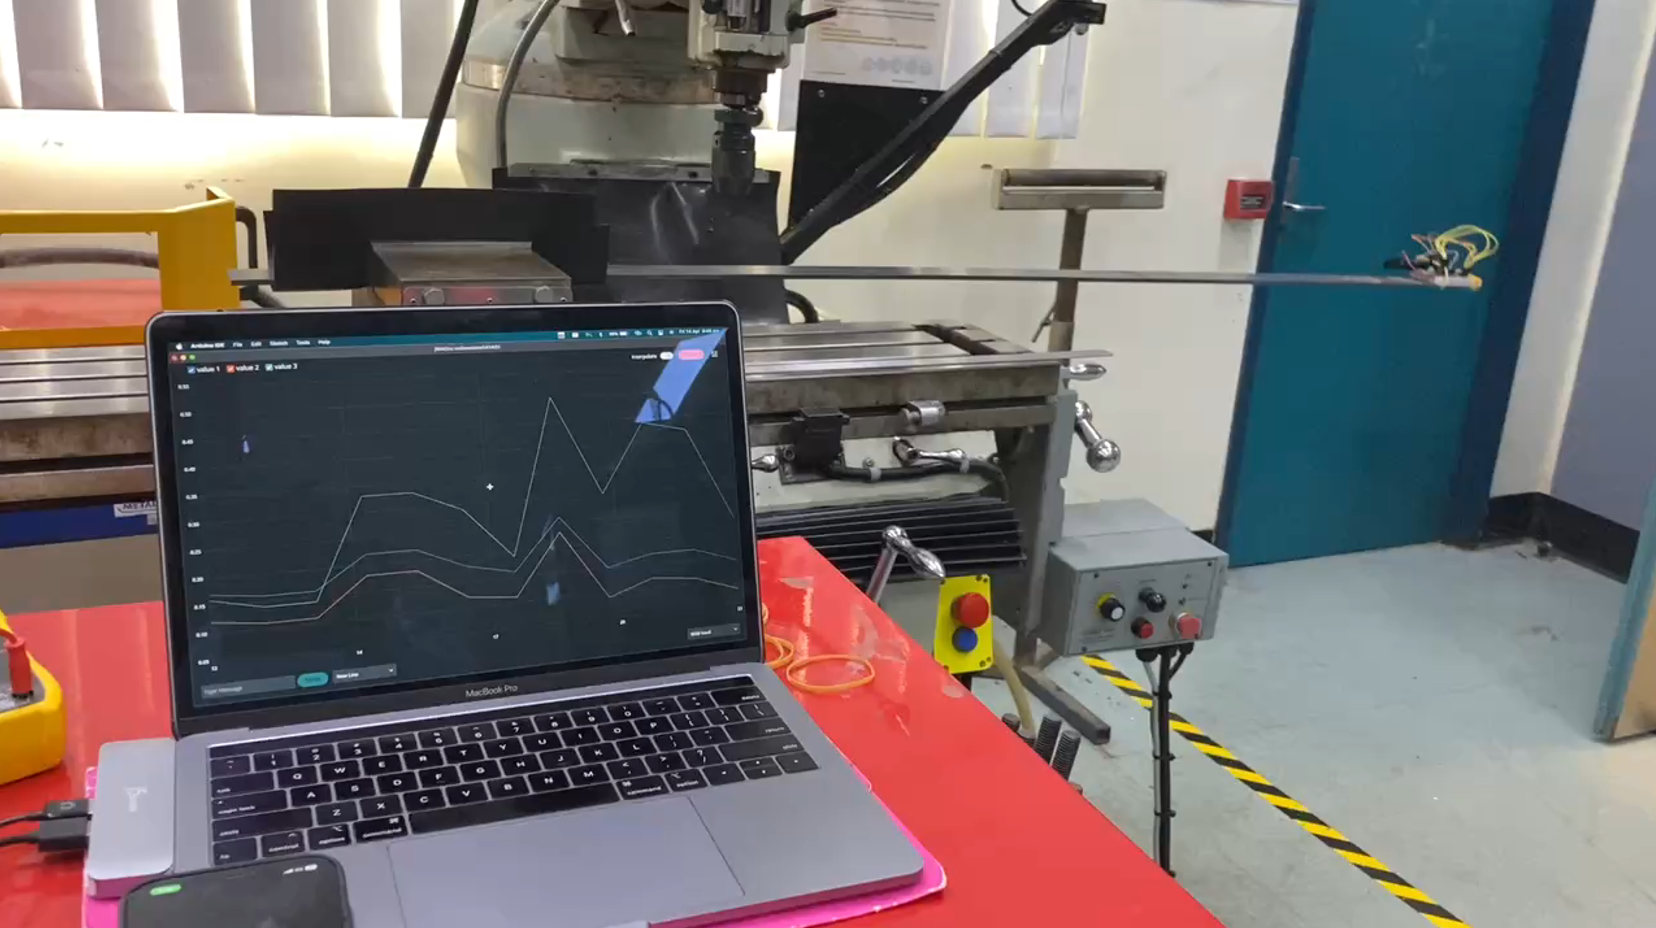
\includegraphics[width=\textwidth]{Sections/Prototype-Testing/beam-test-setup.png}
	\label{beam-test-setup}
\end{figure}

Initially, the noise threshold values in the acceleration processing function were tuned through trial and error. The live serial plot in Arduino IDE assisted in tuning these parameters to a final value of 0.7 for the x-axis, 0.9 for the y-axis and 0.1 for the z-axis. The beam was then pushed down 15cm and released. Once the noise thresholds were acceptable, the first test was conducted. 

\subsubsection{Prototype 1: Test 1}
Test one involved two participants, one to monitor the laptop and run the software and another to push the beam down. The first test was conducted with both devices connected to the laptop via USB. The node device was fastened to the beam and the reset button was pushed, calibrating the device. The node device on the beam can be seen in figure \ref{node-beam-test}. The sender and receiver Python logging scripts were executed on the laptop, as seen in figure \ref{laptop-beam-test}, and the beam was released. The test ran for approximately two minutes until the beam reached a stationary state. At this moment the logging programs were ended and the sender and receiver Python plotting scripts were executed. The names of each logging file was input by the user and the raw acceleration, maximum acceleration and peak frequency were displayed in a pyplot graph. These graphs were named and saved as PNG files. 

\begin{figure}[H]
	\centering
	\begin{subfigure}{.5\textwidth}
		\centering 
		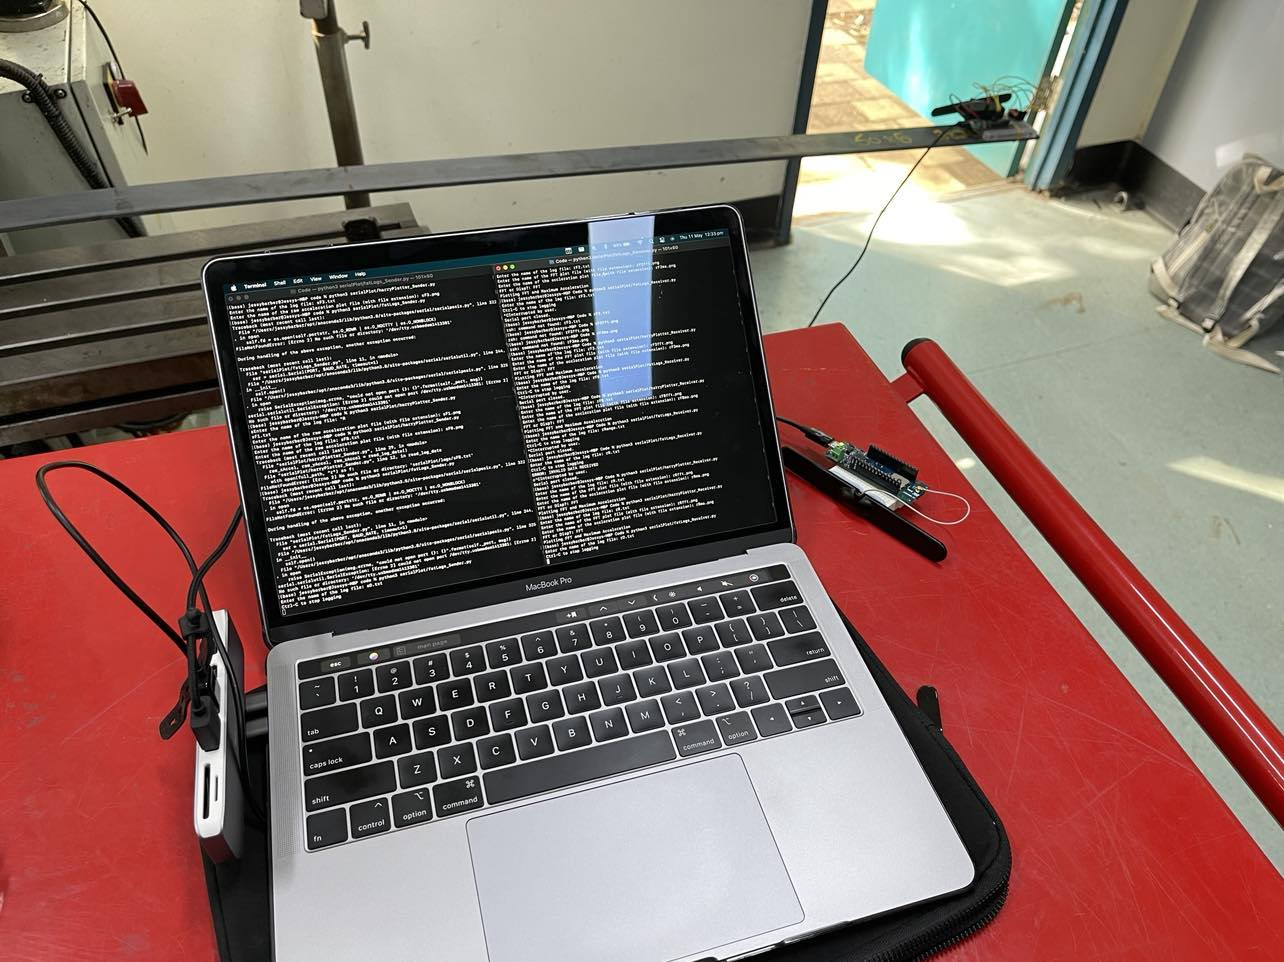
\includegraphics[scale=0.15]{Sections/Prototype-Testing/laptop-beam-test.jpg}
		\caption{Logging Python Scripts}
		\label{laptop-beam-test}
	\end{subfigure}%
	\begin{subfigure}{.25\textwidth}
		\centering
		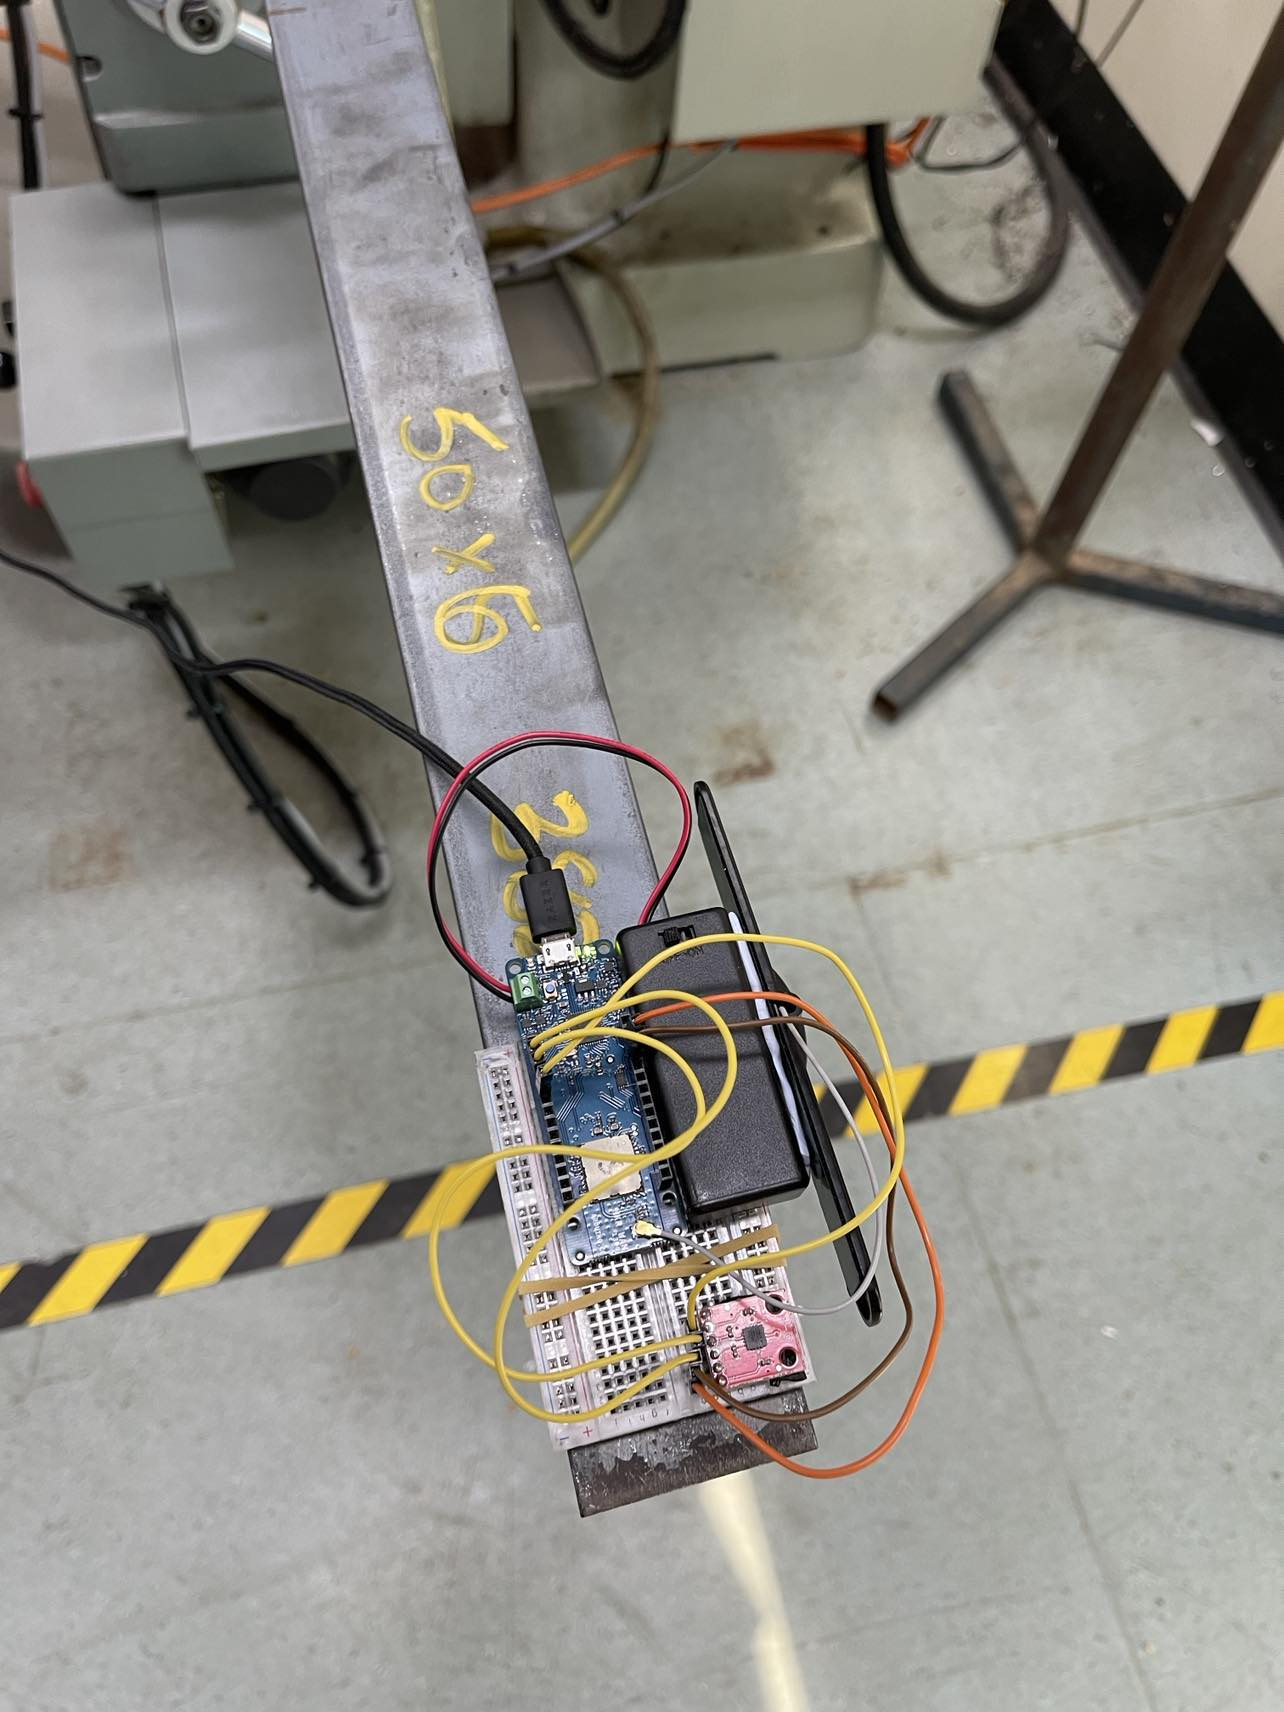
\includegraphics[scale=0.1]{Sections/Prototype-Testing/node-beam-test.jpg}
		\caption{Node Device on Beam}
		\label{node-beam-test}
	\end{subfigure}
	\caption{Close Up of Laptop and Node with Serial Connection in Beam Test}
	\label{close-beam-test}
\end{figure}

\subsubsection{Prototype 1: Test 1 Results}
Figure \ref{proto1-test1-ra} shows the raw acceleration from the serial connection between the node device and laptop and figures \ref{proto1-test1-ma} and \ref{proto1-test1-f} show the maximum acceleration and maximum frequency from the serial connection between the gateway device and the laptop. The raw and maximum acceleration are characteristic of the beam accelerating with maximum displacement and decaying over time to the stationary position. The peak frequency from the FFT is 2.4 Hz which matches the first mode fundamental frequency achieved in the Strand7 FE simulation shown in figures \ref{strand7-simulation} and \ref{strand7-results}. This verifies that the FFT computation can accurately identify the maximum peak frequency. 

\begin{figure}[H]
	\centering
	\caption{Beam Test FE Simulation}
	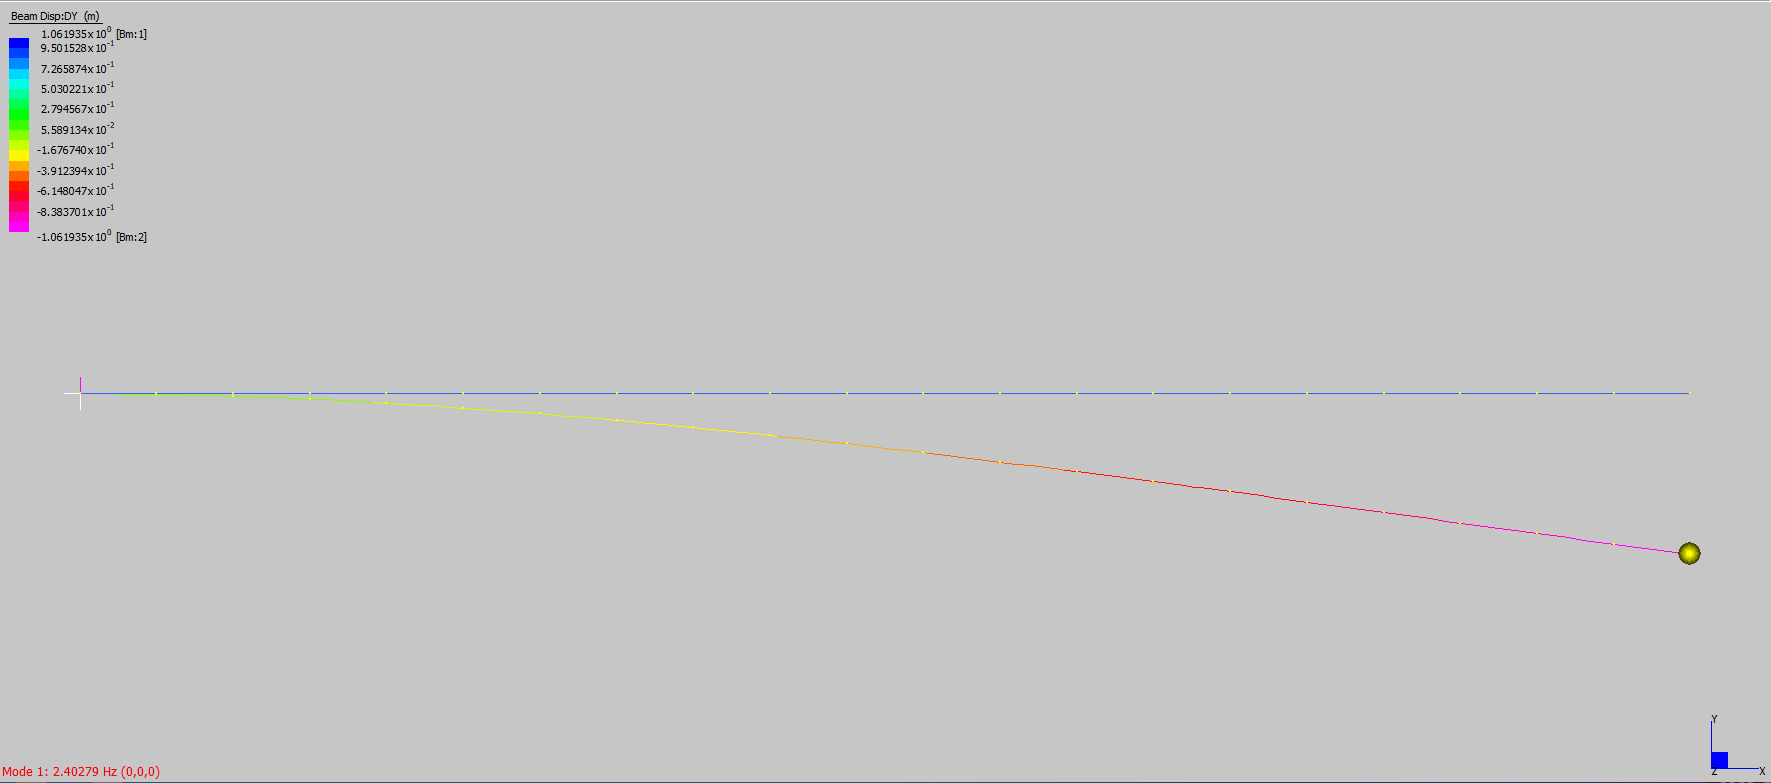
\includegraphics[width=\textwidth]{Sections/Prototype-Testing/strand7-simulation.png}
	\label{strand7-simulation}
\end{figure}

\begin{figure}[H]
	\centering
	\caption{Beam Test FE Simulation Results}
	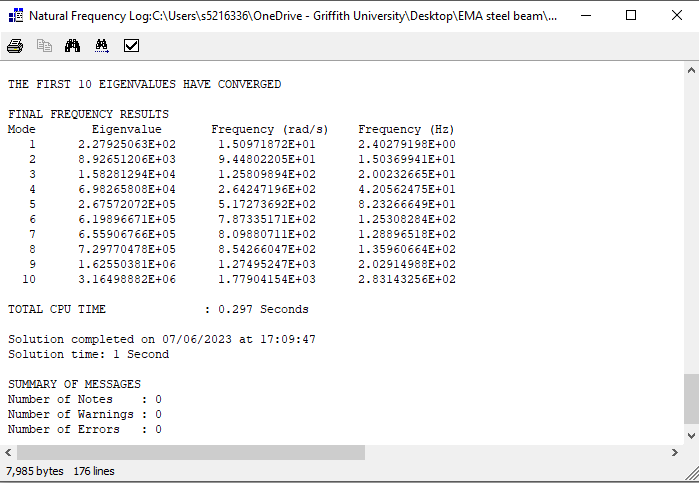
\includegraphics[width=\textwidth]{Sections/Prototype-Testing/strand7-results.png}
	\label{strand7-results}
\end{figure}

\begin{figure}[H]
	\centering
	\caption{Prototype 1: Test 1 Raw Acceleration}
	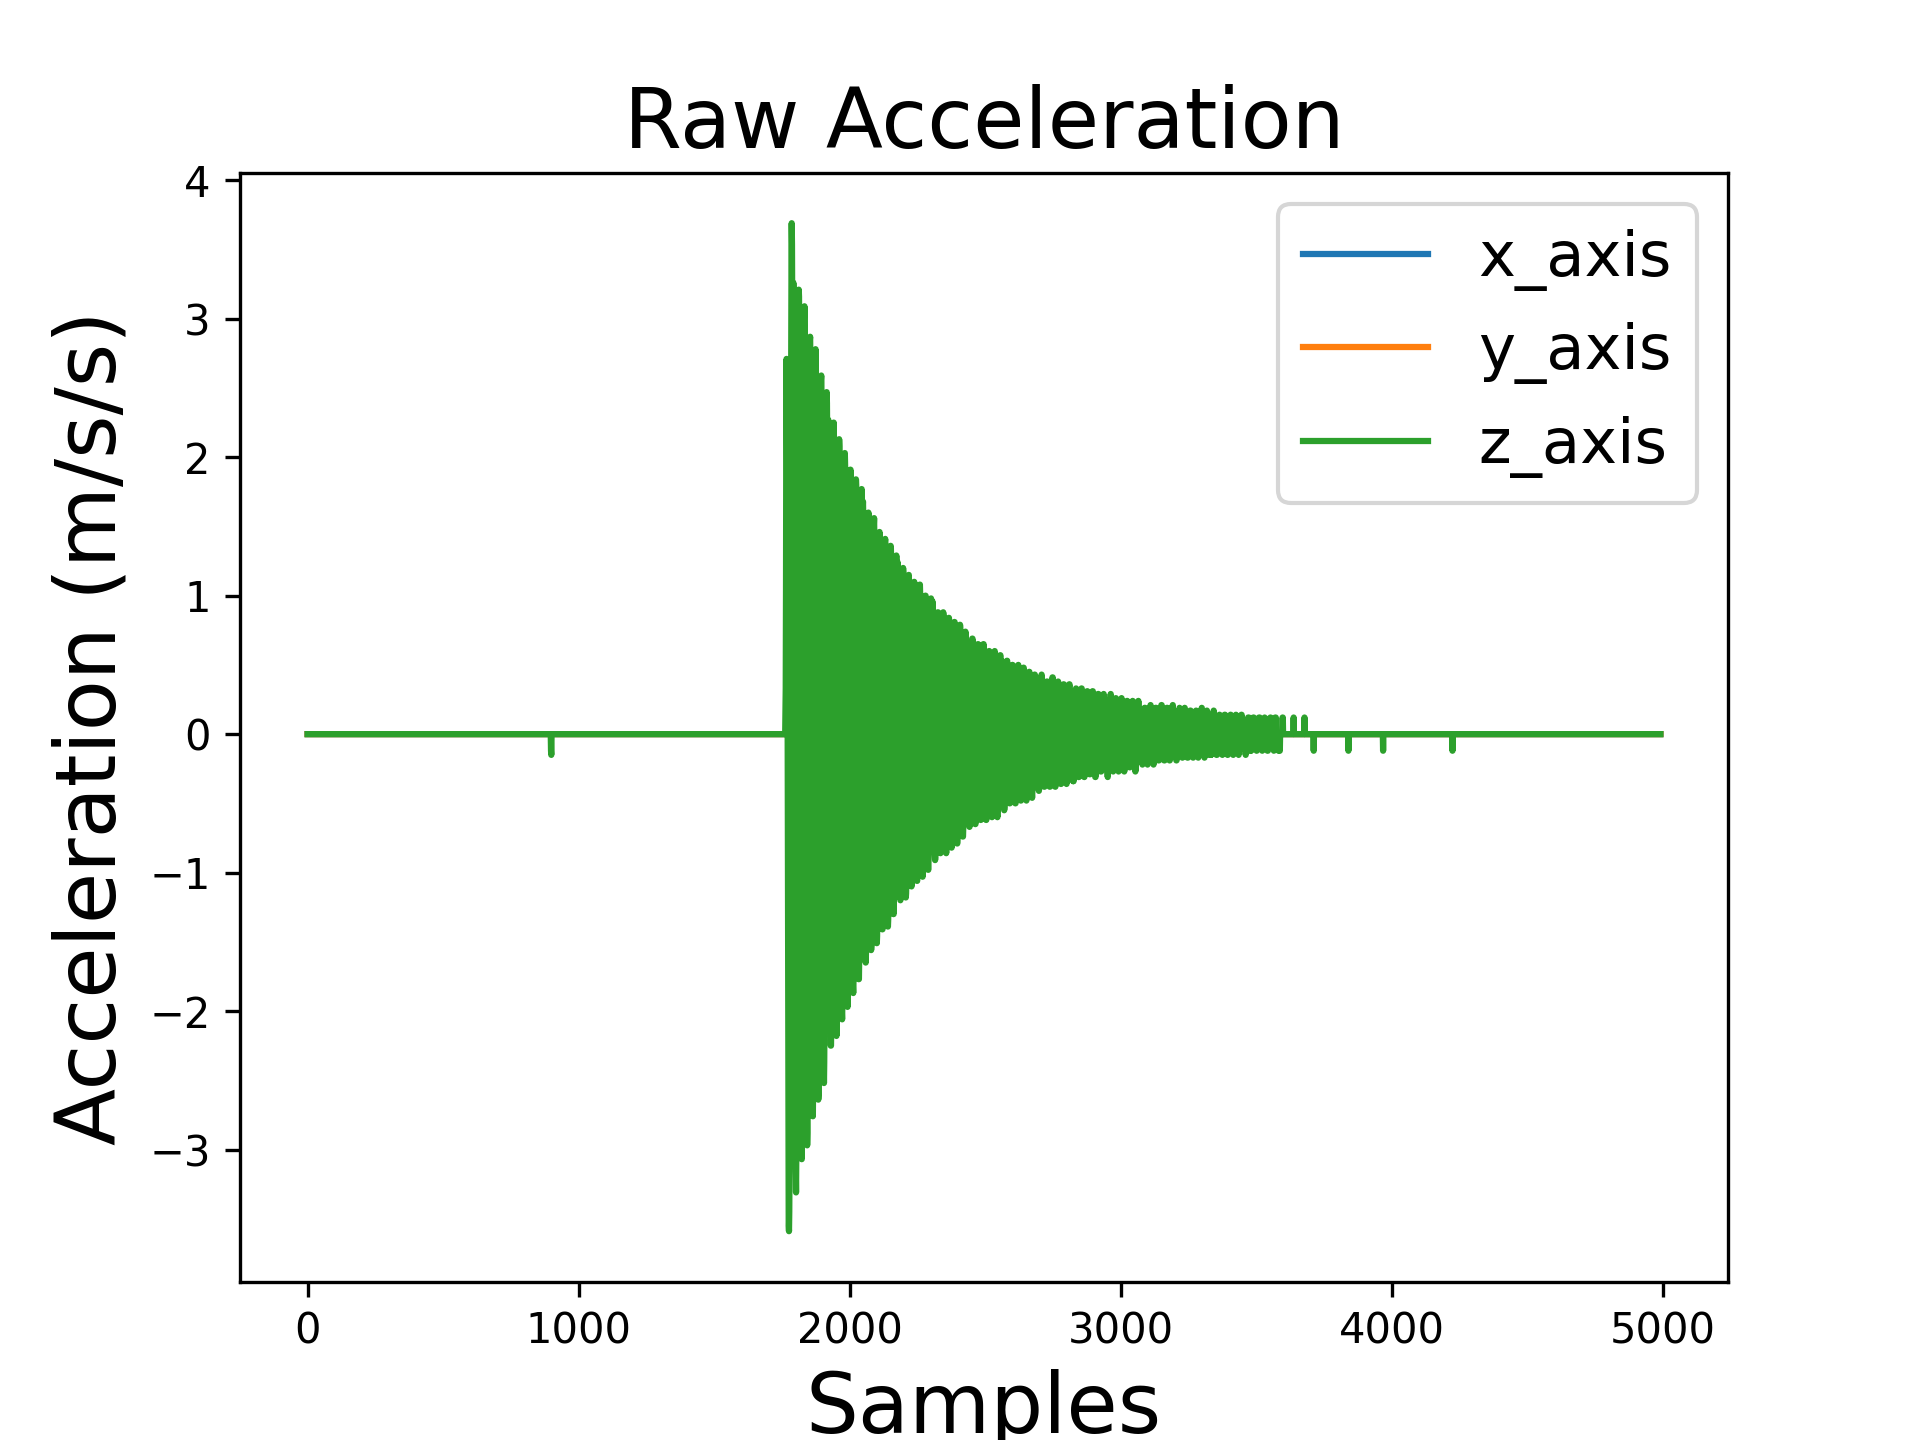
\includegraphics[width=.9\textwidth]{Sections/Prototype-Testing/PosterRA.png}
	\label{proto1-test1-ra}
\end{figure}

\begin{figure}[H]
	\centering
	\caption{Prototype 1: Test 1 Maximum Acceleration}
	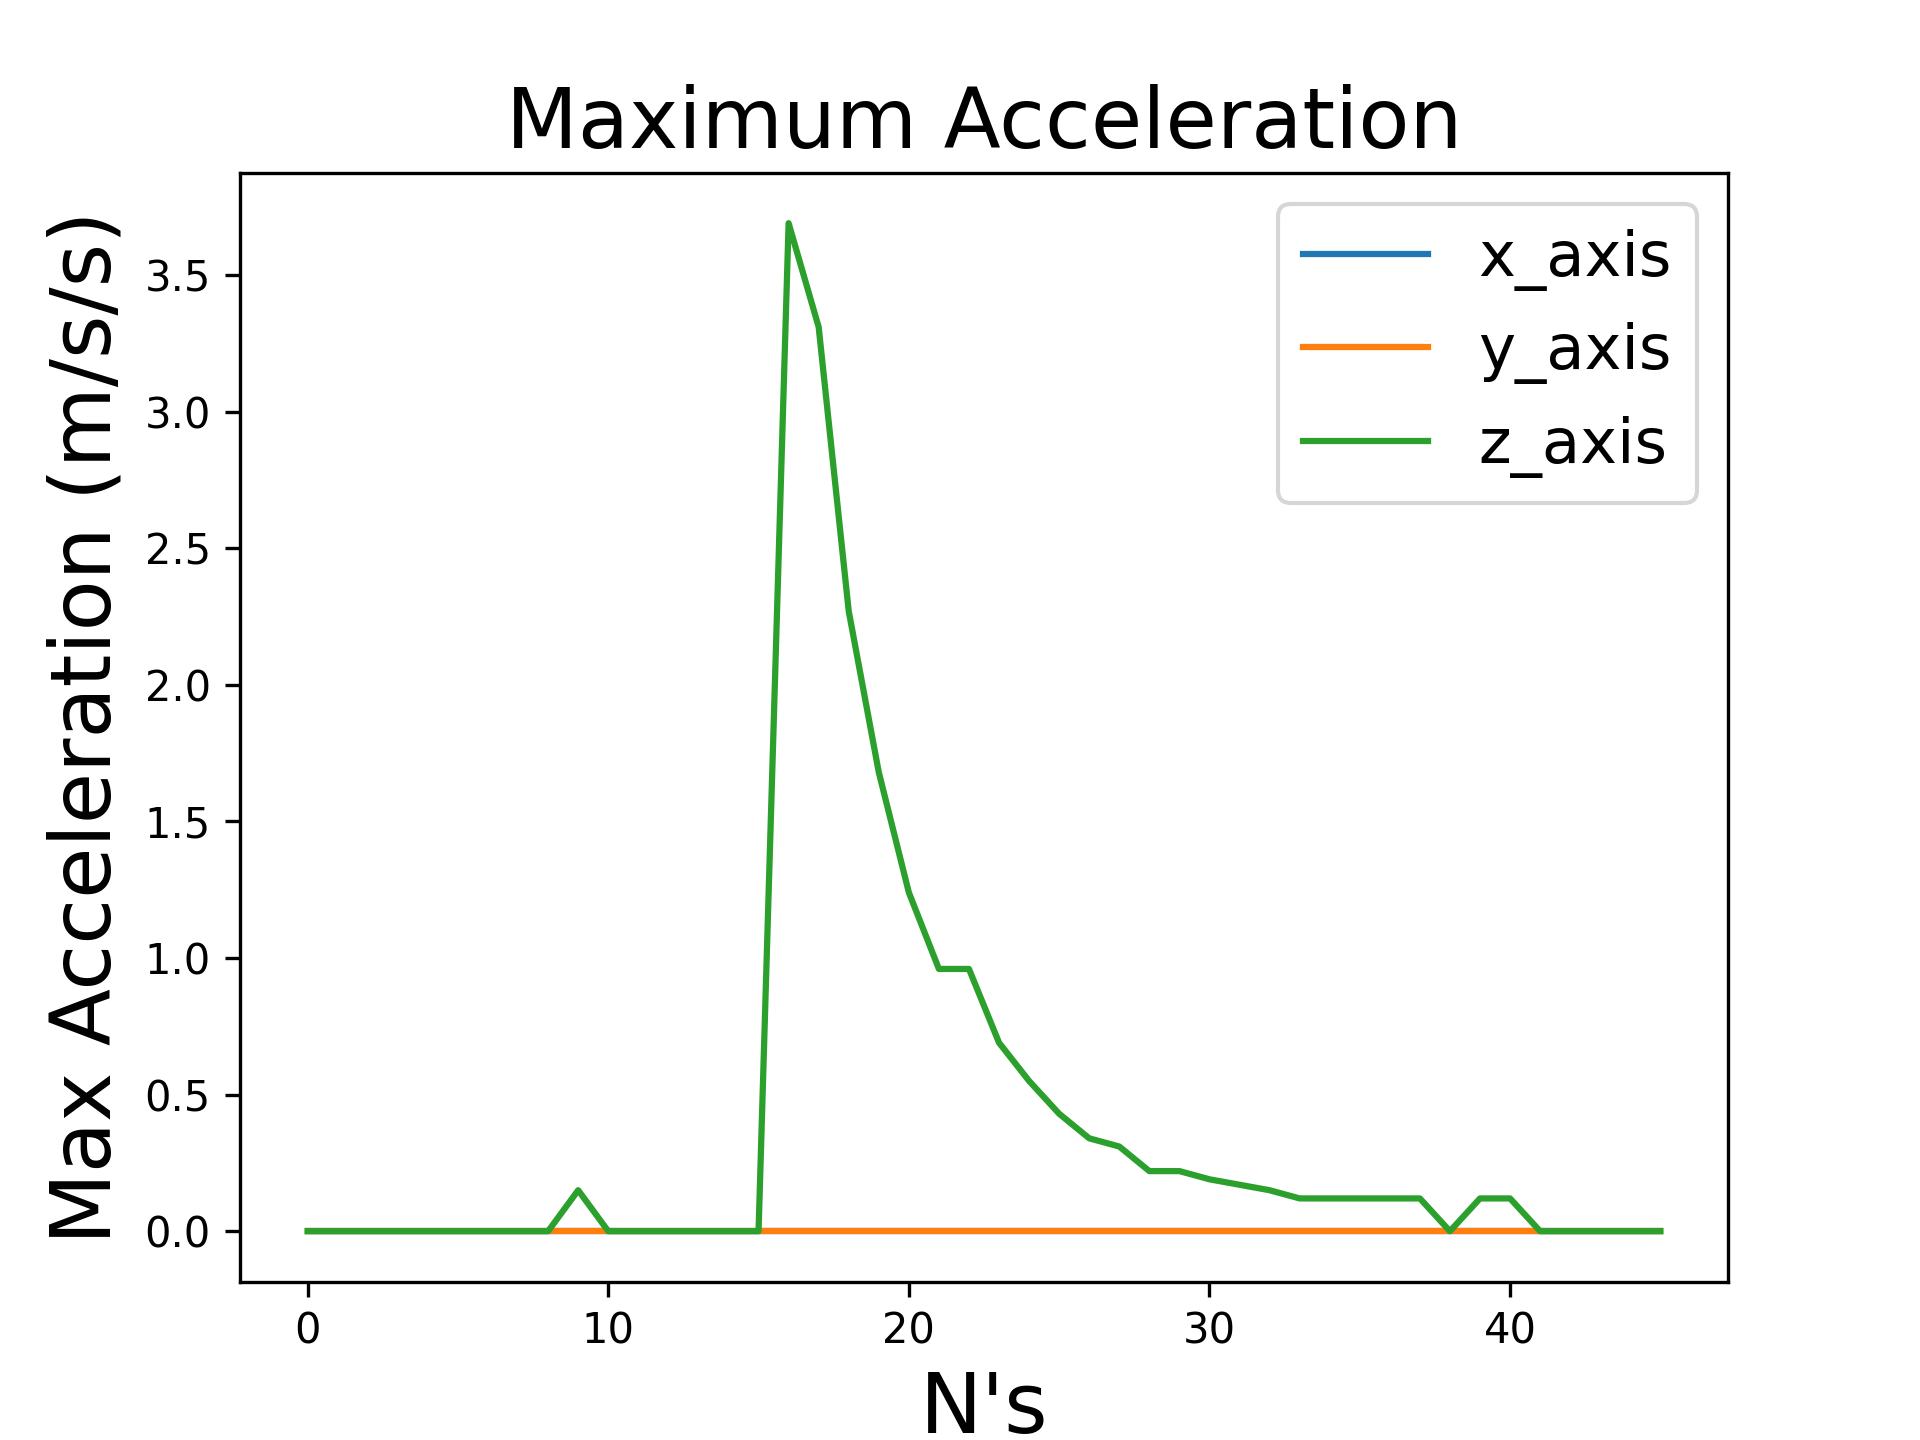
\includegraphics[width=.9\textwidth]{Sections/Prototype-Testing/PosterMA.png}
	\label{proto1-test1-ma}
\end{figure}

\begin{figure}[H]
	\centering
	\caption{Prototype 1: Test 1 Maximum Frequency}
	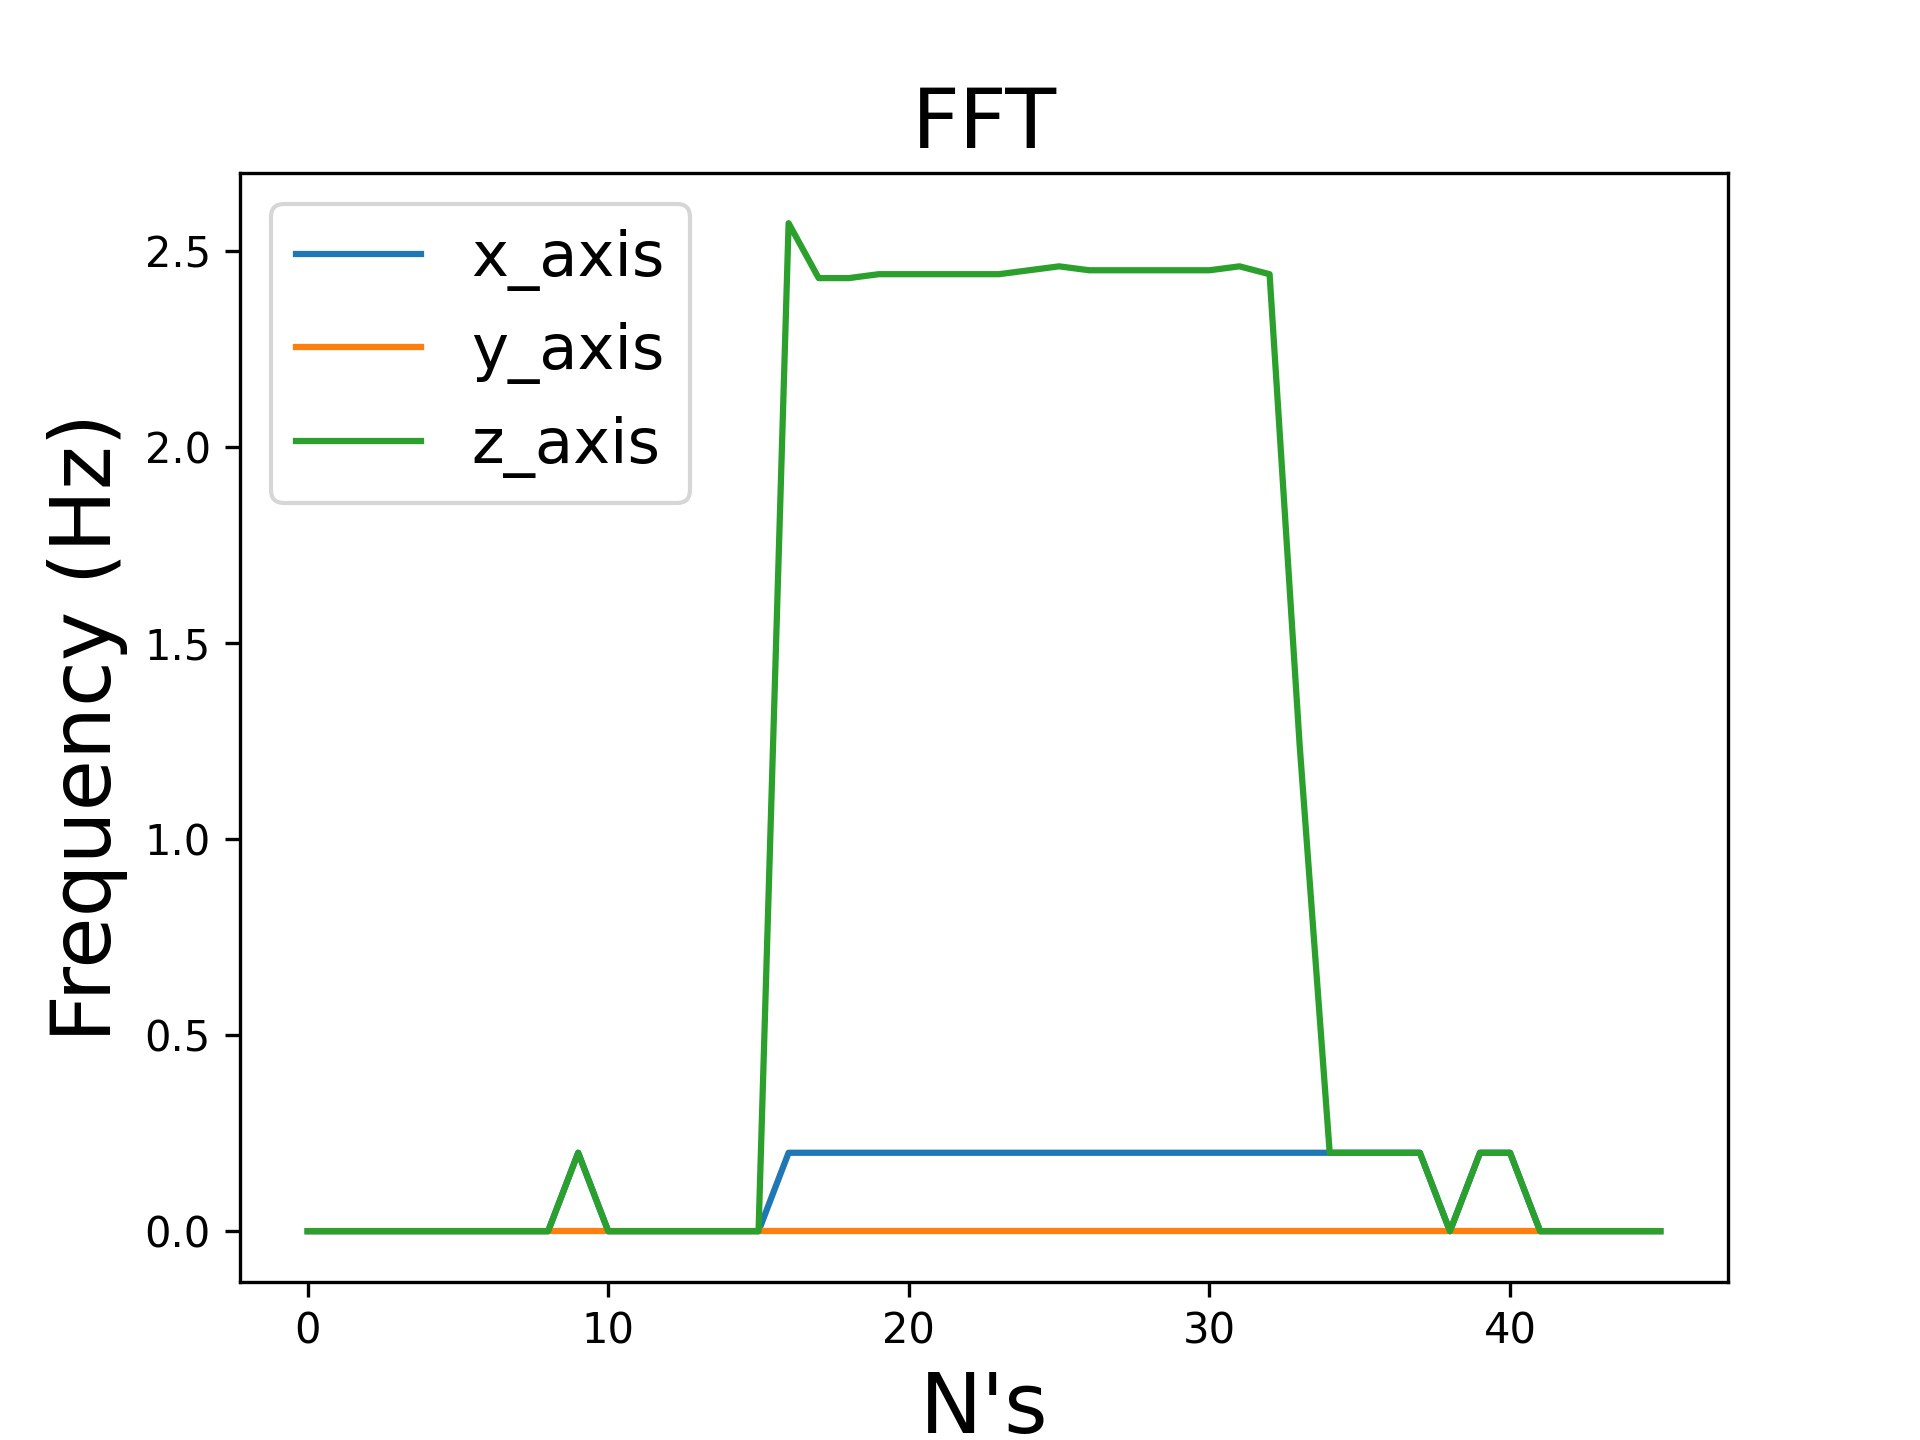
\includegraphics[width=.9\textwidth]{Sections/Prototype-Testing/PosterF.png}
	\label{proto1-test1-f}
\end{figure}

\subsubsection{Prototype 1: Test 2}
Test two removed the serial connection between the node device and the laptop and used the battery pack to power the device instead. The aim of this test was to achieve the same results as test one with a different input voltage and no serial connection for the node device. To initiate the test, the battery pack was switched on, and the reset button on the device was pushed, calibrating the accelerometer with the new reference voltage. This time only the receiver Python logging script was executed following the release of the beam. Once the beam reached its resting state the logging script was ended and the receiver Python plotting script was executed. The maximum acceleration and maximum frequency were plotted using pyplot and saved as PNG files. Figure \ref{beam-test-wireless} displays the node device on the beam with no physical connection to the laptop. 

\subsubsection{Prototype 1: Test 2 Results}
Figures \ref{proto1-test2-ma} and \ref{proto1-test2-f} show the maximum acceleration and maximum frequency from the serial connection between the gateway device and the laptop. These results show the same response as test one which verify the capability of the device running from the battery pack and successful calibration of the accelerometer when using a lower reference voltage of 3.0V. 

\begin{figure}[H]
	\centering
	\caption{Wireless Node in Beam Test}
	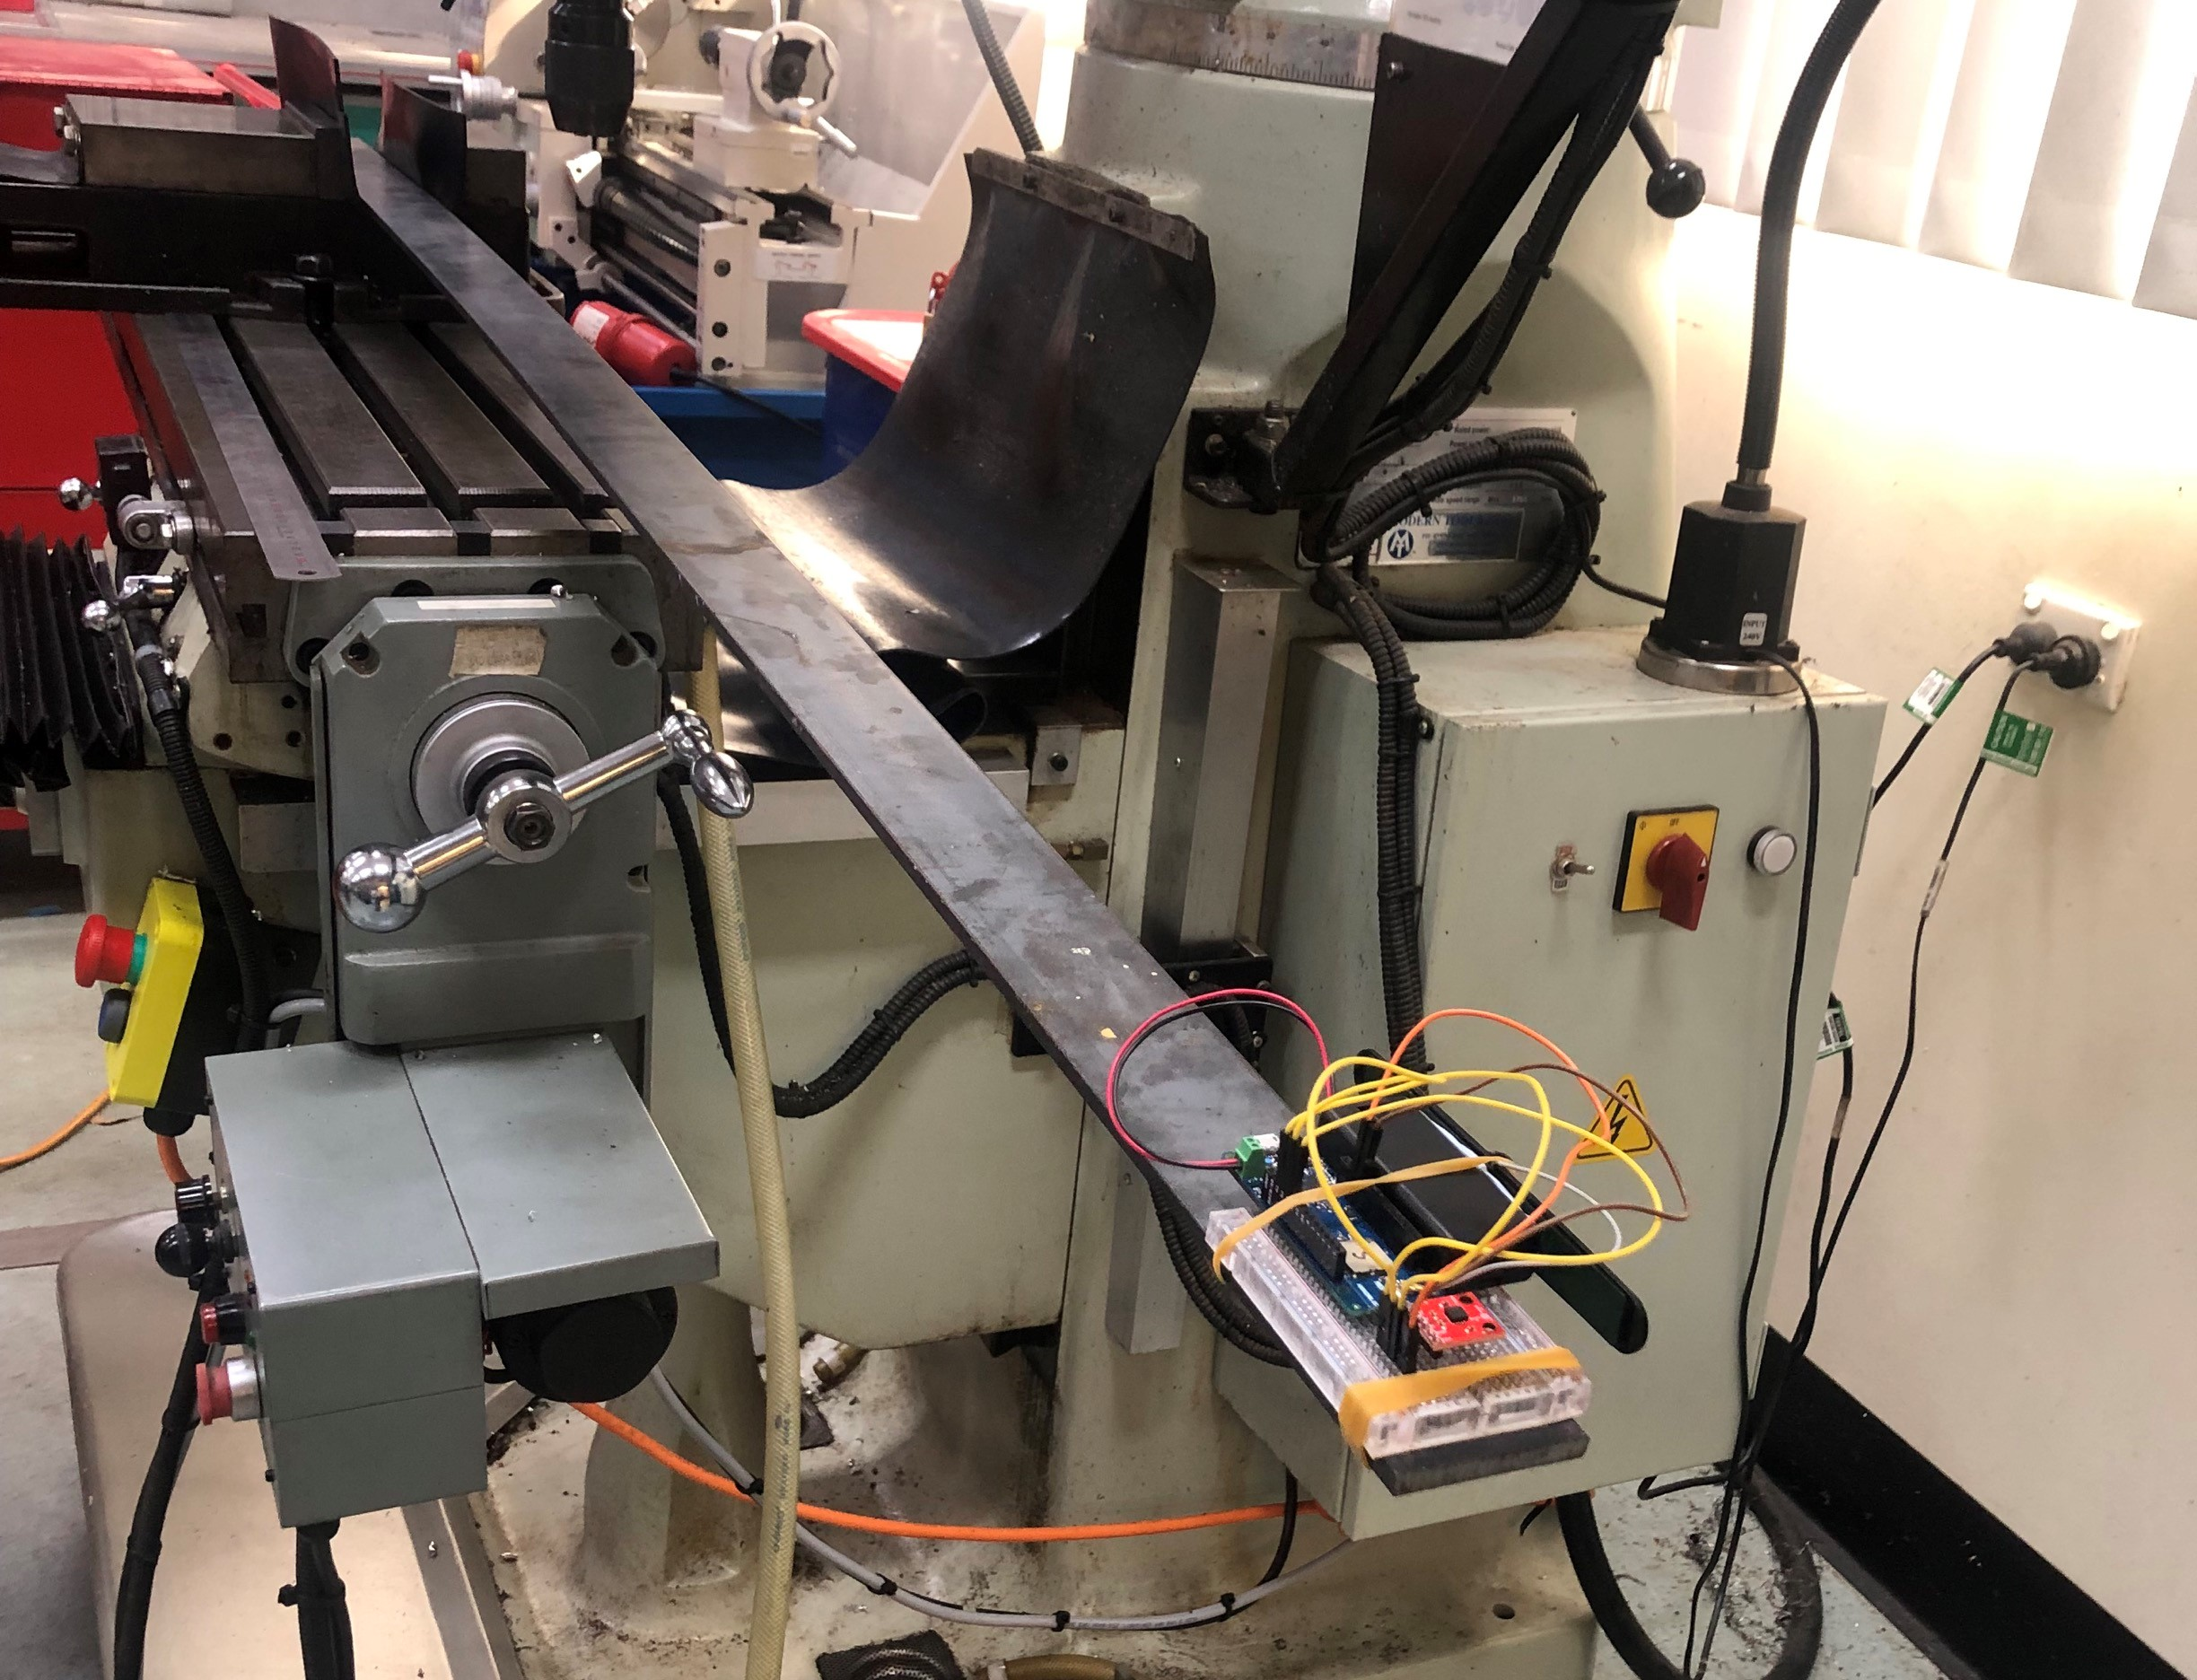
\includegraphics[width=.8\textwidth]{Sections/Prototype-Testing/beam-test-wireless.png}
	\label{beam-test-wireless}
\end{figure}

\begin{figure}[H]
	\centering
	\caption{Prototype 1: Test 2 Maximum Acceleration}
	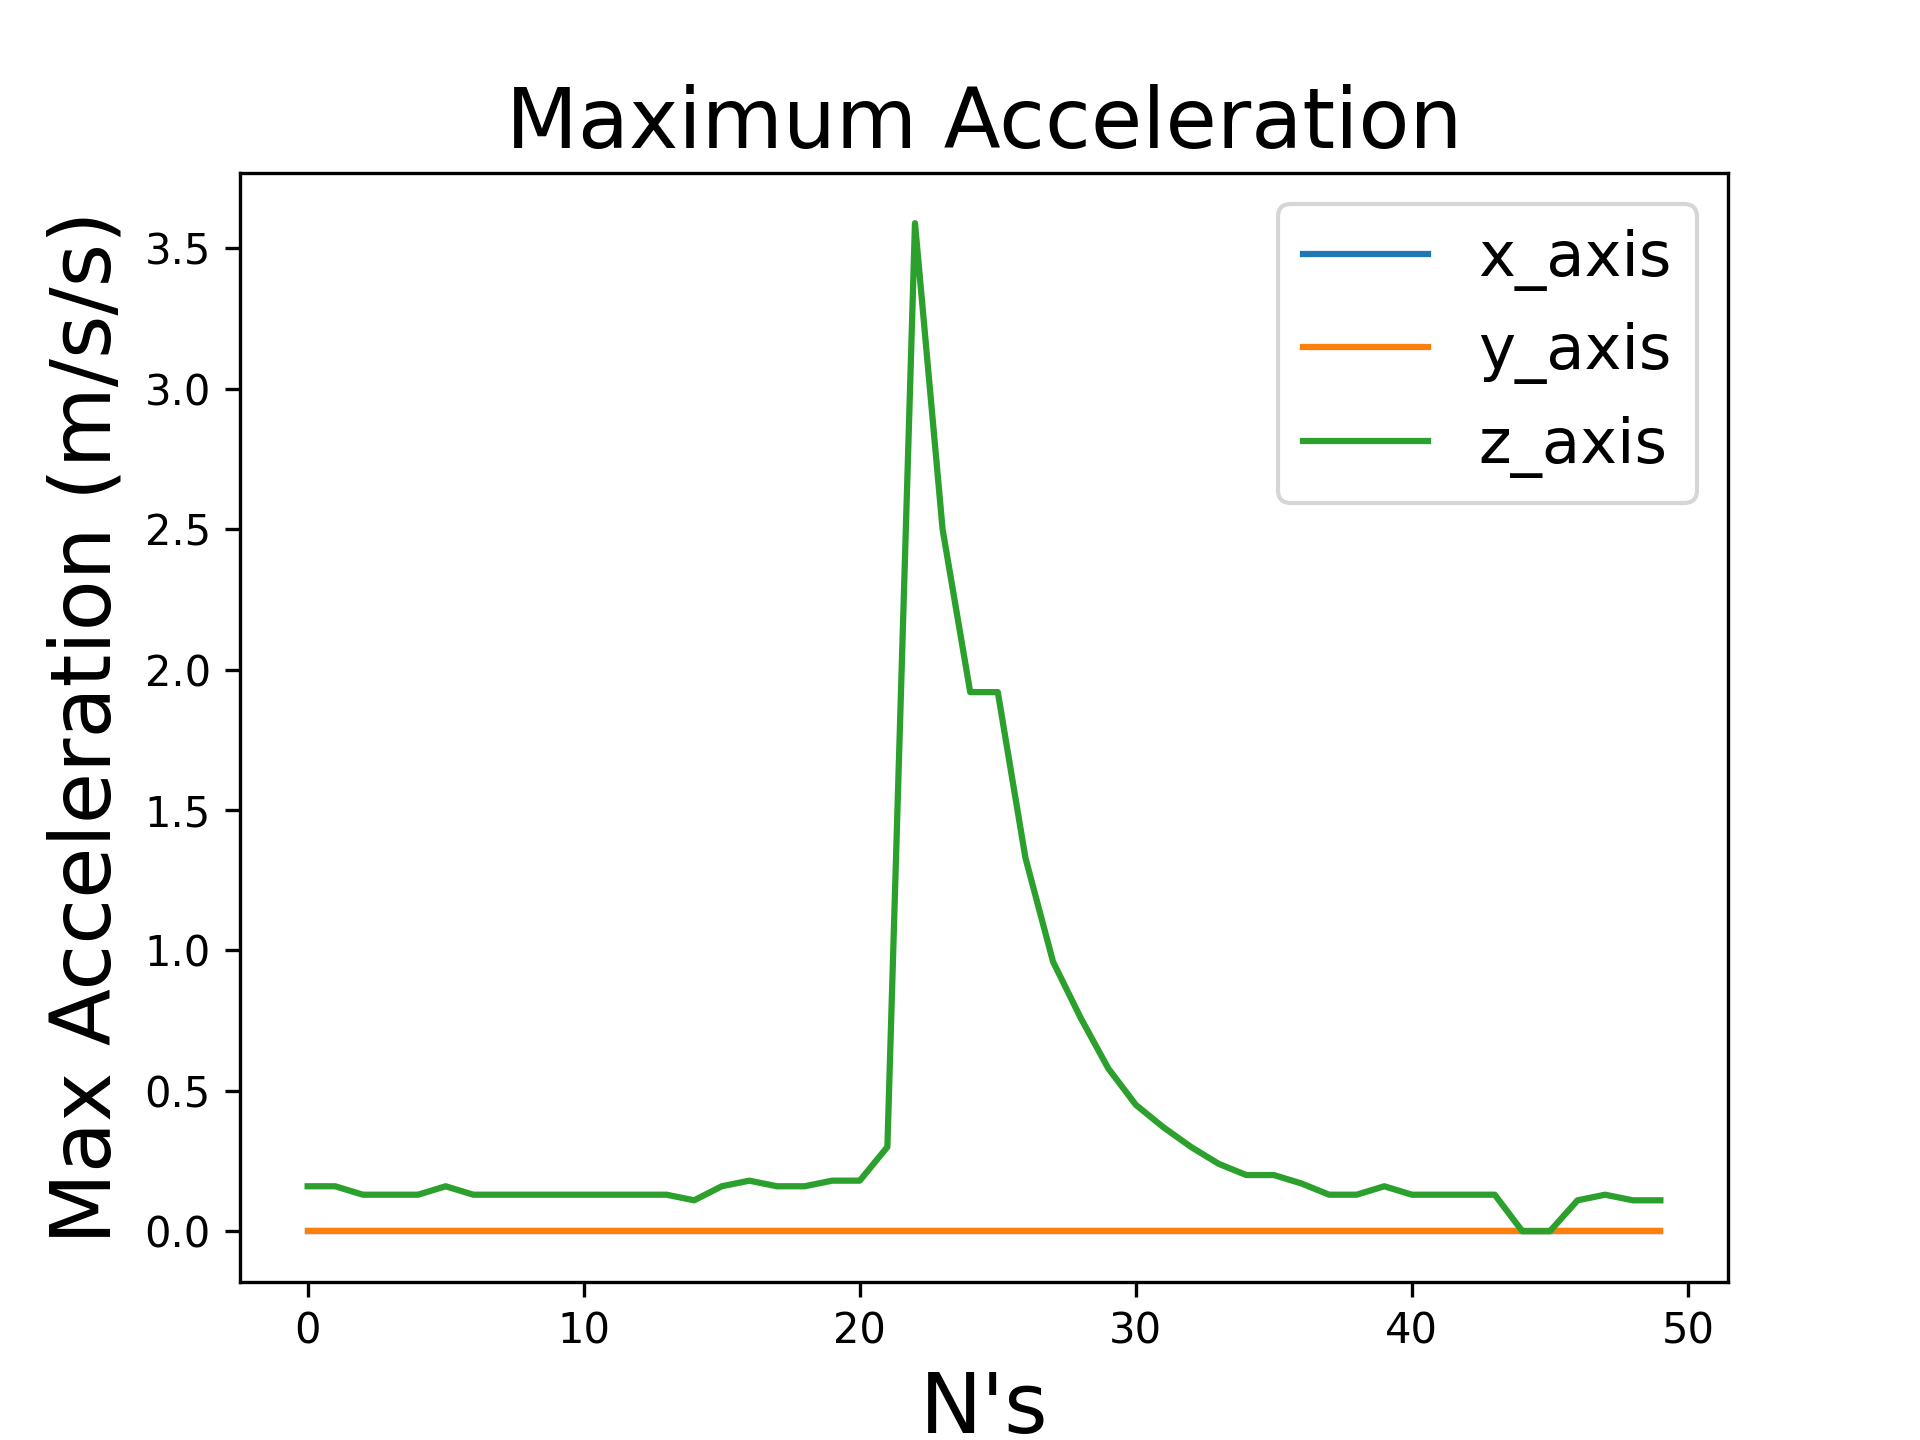
\includegraphics[width=.9\textwidth]{Sections/Prototype-Testing/test2-ma.png}
	\label{proto1-test2-ma}
\end{figure}

\begin{figure}[H]
	\centering
	\caption{Prototype 1: Test 2 Maximum Frequency}
	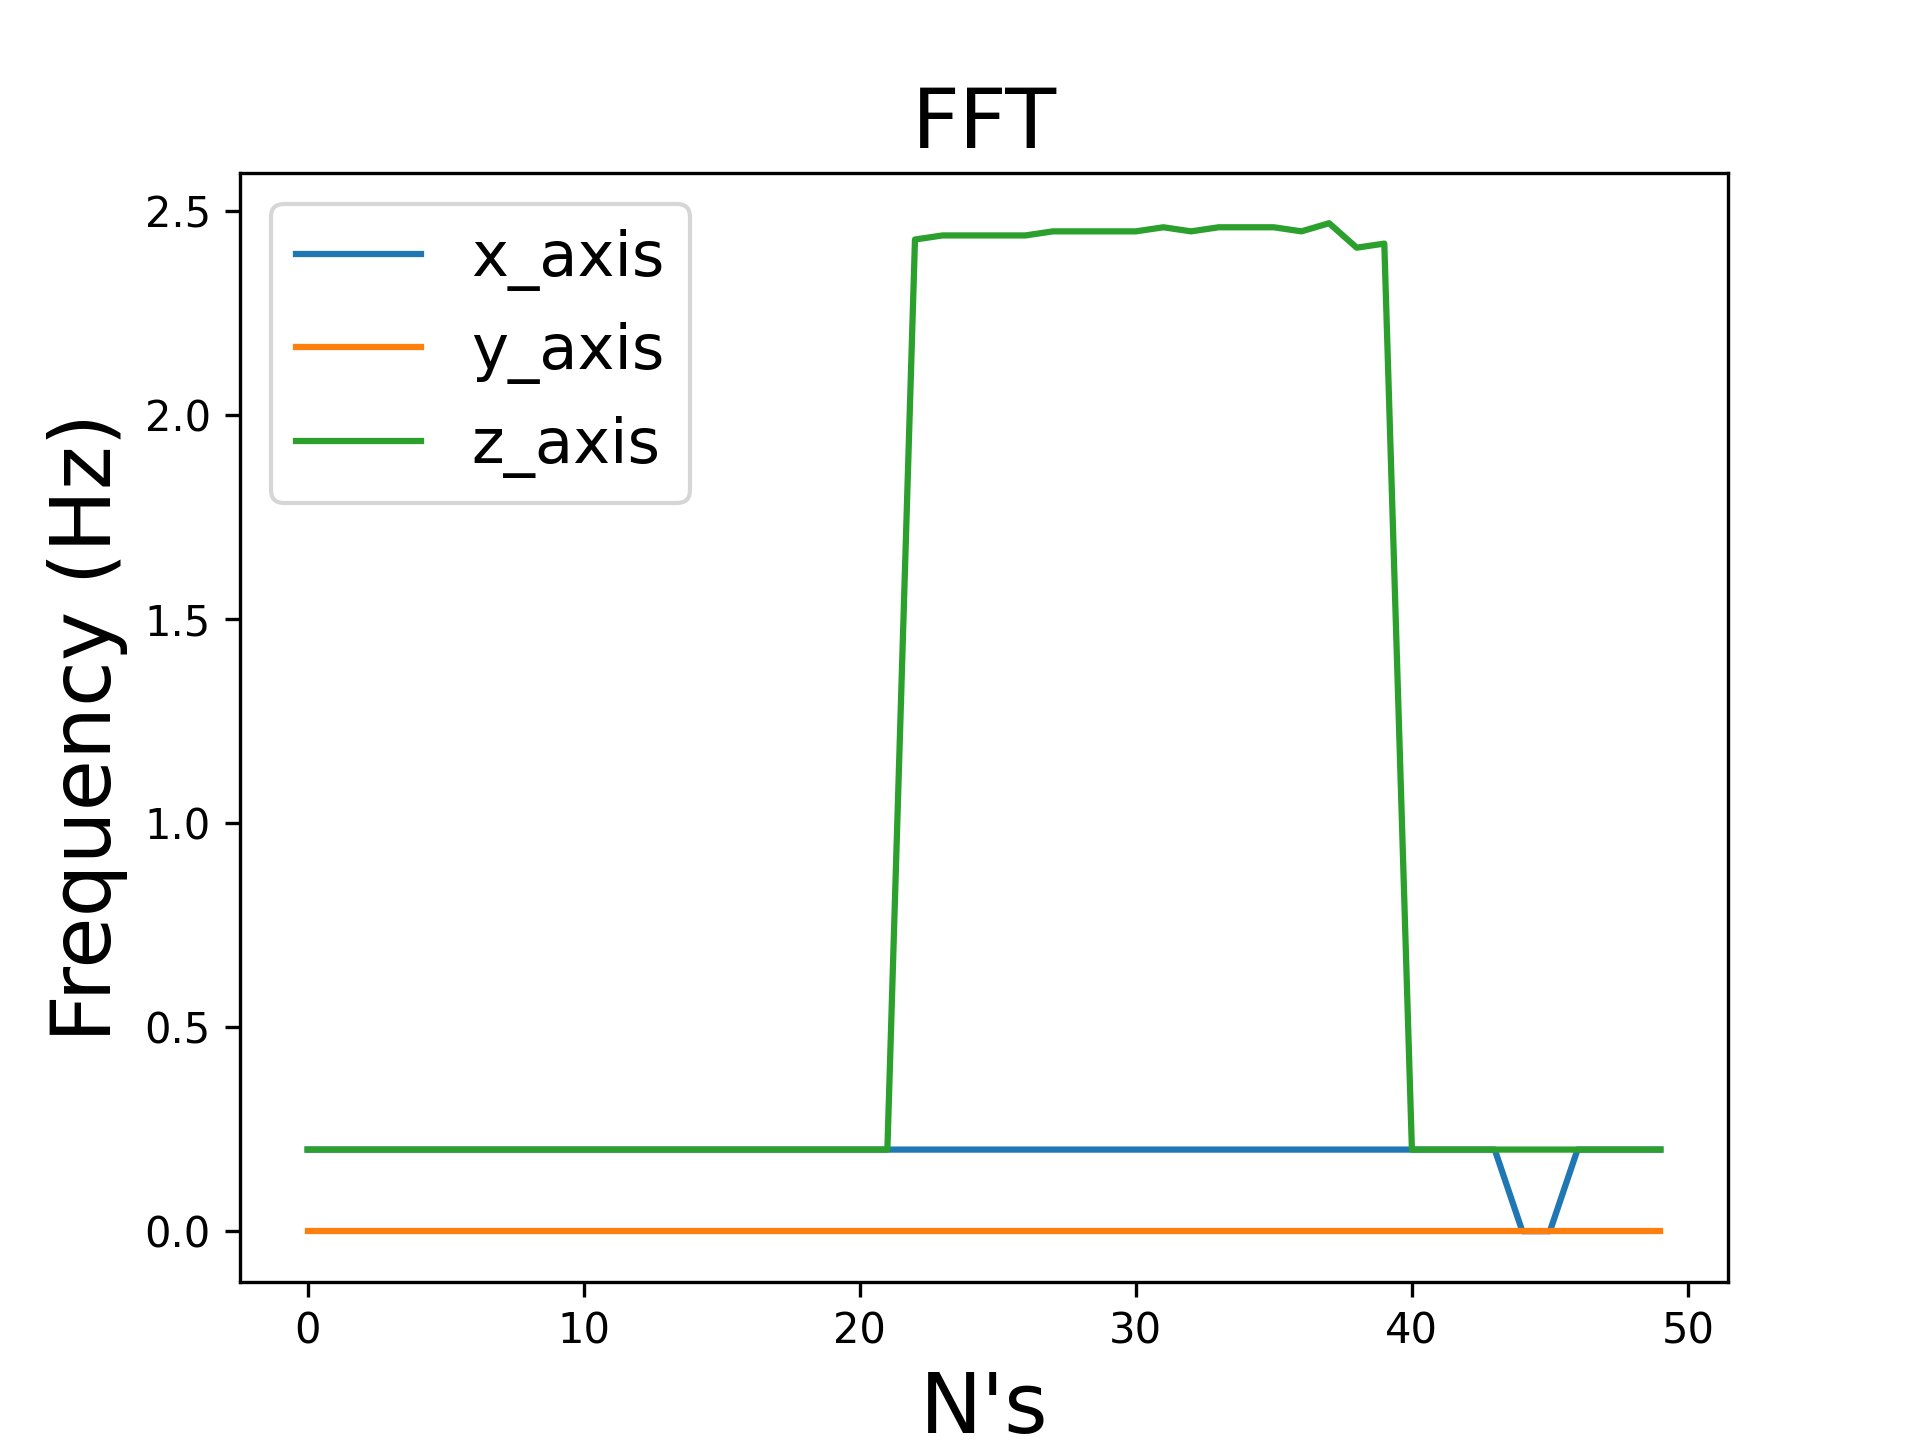
\includegraphics[width=.9\textwidth]{Sections/Prototype-Testing/test2-f.png}
	\label{proto1-test2-f}
\end{figure}

\subsubsection{Prototype 1: Test 3}
The purpose of test three was to test the range of the communication between the two devices. To do this one participant stayed in the laboratory and the other carried the laptop away with the gateway node which was still connected serially. A Microsoft Teams call was used to communicate between the two participants during this test. The beam was continuously pushed down and the data was observed on the Arduino IDE's live serial plotter. The test was ended once the gateway node was unable to receive LoRa packets and the location was recorded. 

\subsubsection{Prototype 1: Test 3 Results}
Figure \ref{proto1-test3-range} shows the maximum range of successful communication between the two devices. The range was measured between the mechanical engineering laboratory and the start of the Griffith footbridge, reaching a distance of approximately 200m. 

\begin{figure}[H]
	\centering
	\caption{Prototype 1: Test 3 Range \cite{test3-range}}
	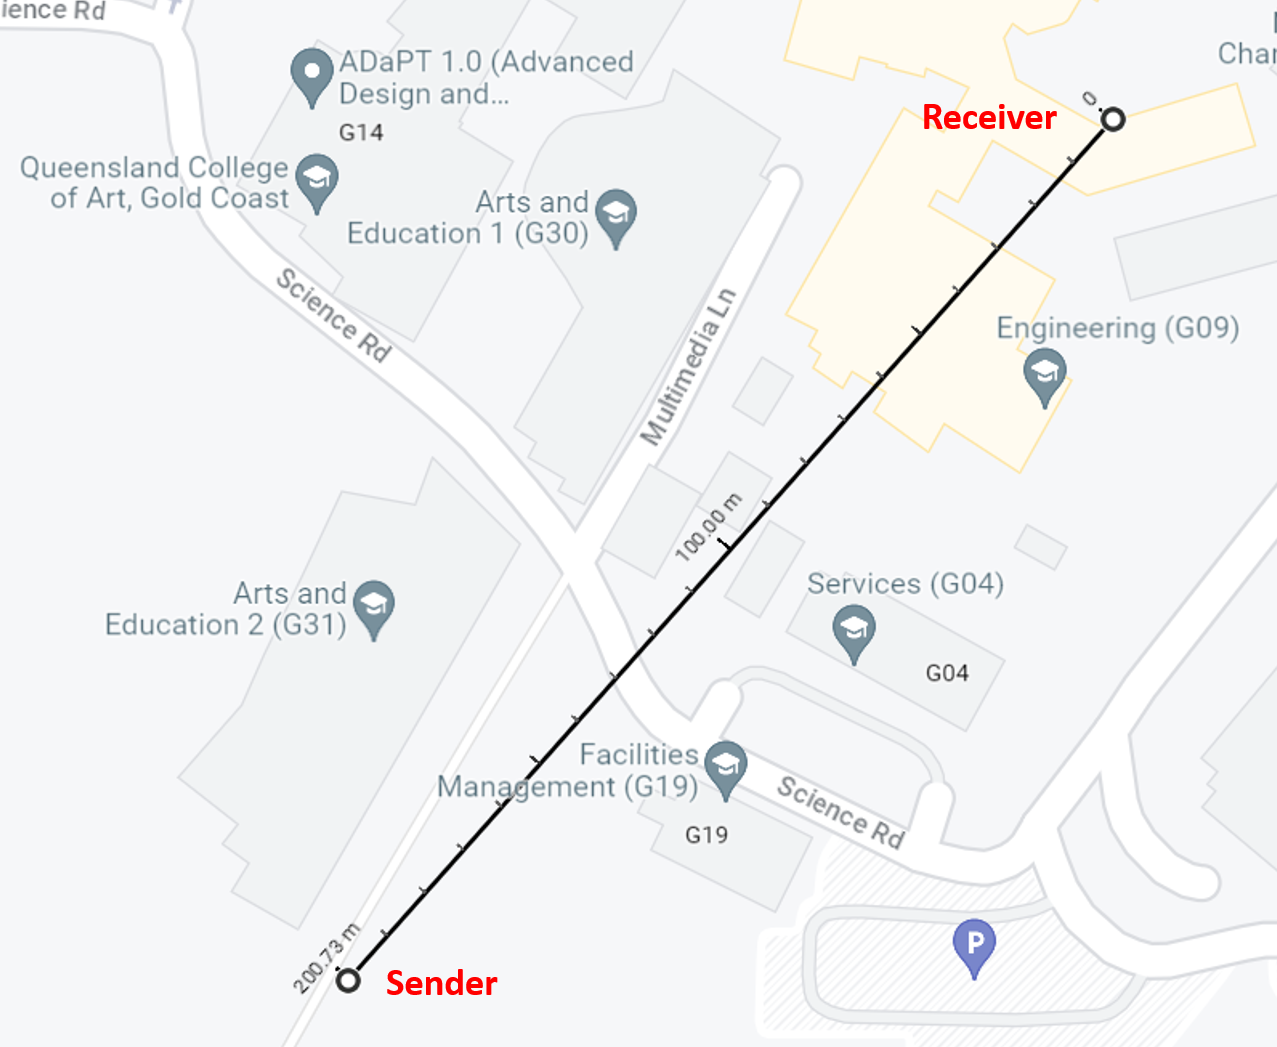
\includegraphics[width=\textwidth]{Sections/Prototype-Testing/test3-range-label.png}
	\label{proto1-test3-range}
\end{figure}

\subsection{Prototype 2: Bridge Test}
The purpose of the bridge test was to test a full deployment of IoT architecture for structural health monitoring and to verify the first mode flexural frequency stated in the Griffith footbridge documentation. This test involved installing the enclosure behind the hand rail of the footbridge and setting up a base station for data collection. The base station was placed 25m away from the node device and consisted of a power generator, laptop and LoRaWAN gateway. Similar to the prototype one testing, the noise threshold values were fine tuned over the course of several experiments. The Arduino IoT Cloud dashboard was used to monitor the data live feed, figure \ref{dashboard}, and the TNN live data page, figure \ref{tnn-live}, was used to observe incoming LoRa packets. The base station can be seen in figure \ref{base-station} and the enclosure installation can be seen in figure \ref{enclosure-integration}. The testing was conducted between 4:00 pm and 6:00pm and the bridge was subjected to moderate pedestrian load from the university and a nearby school. 

\begin{figure}[H]
	\centering
	\caption{Base Station Setup}
	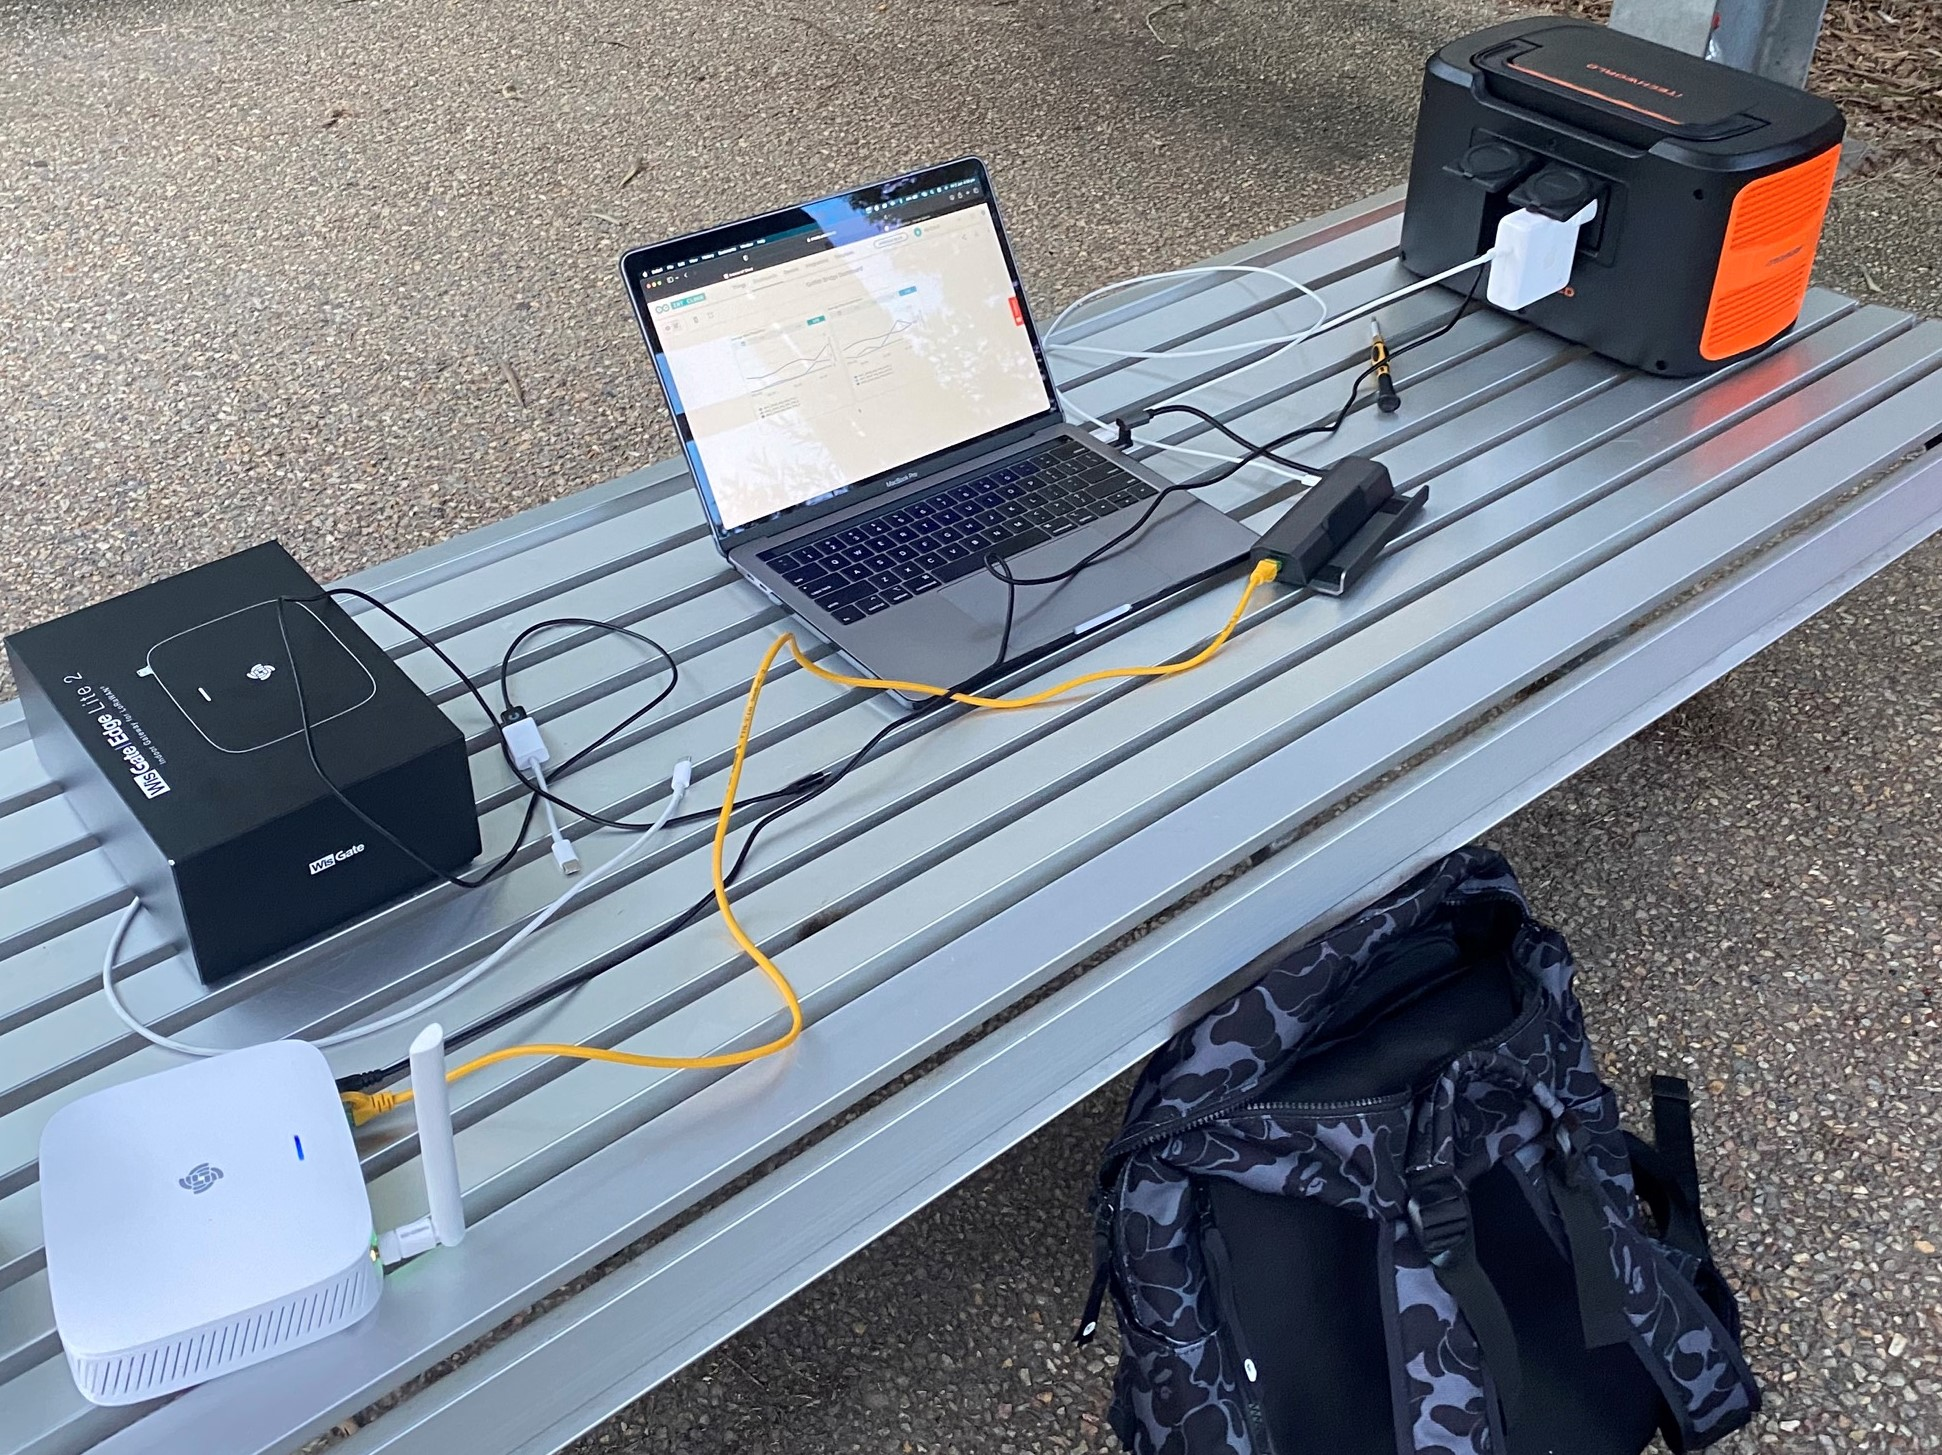
\includegraphics[width=\textwidth]{Sections/Prototype-Testing/base-station.png}
	\label{base-station}
\end{figure}

\subsubsection{Prototype 2: Test 1}
Test one was conducted over a thirty minute period with noise threshold values 0.05 for the x-axis, 0.05 for the y-axis and 0.03 for the z-axis. The purpose of this test was to determine if these noise threshold values were suitable for achieving the expected frequency response of the bridge and to observe the signal strength over time. It was discovered in this test that the enclosure lid was too thick and prevented packet transmission so it was removed for testing. Packets were sent from the node device every sixty seconds and these points were plotted in the Arduino IoT Cloud dashboard. Two participants were required for this experiment, one to monitor the incoming packets on the TNN live data page at the base station, and one to safeguard the enclosure on the bridge. Figure \ref{bridge-axis} displays the orientation of each axis with respect to the enclosure placement on the bridge. 

\begin{figure}[H]
	\centering
	\caption{Prototype 2: Test 1 Enclosure Bridge Axis}
	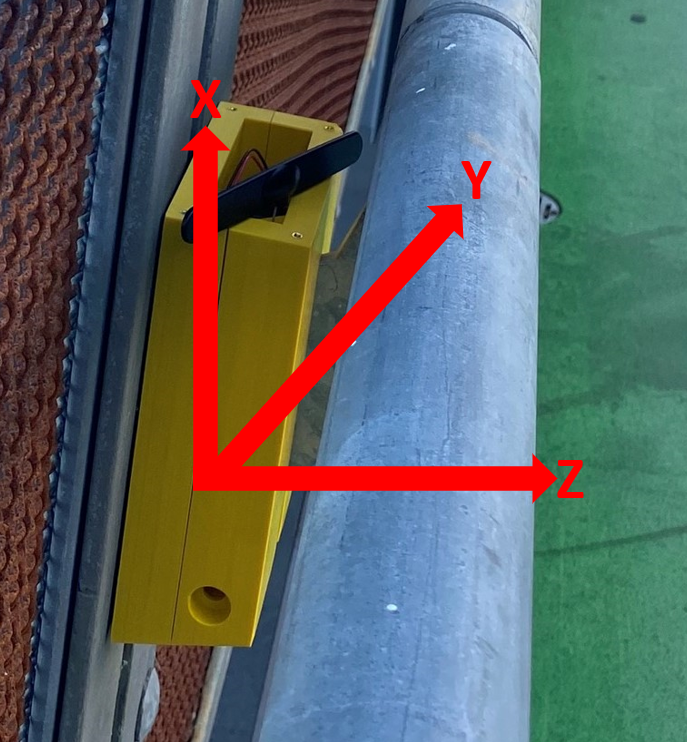
\includegraphics[width=.7\textwidth]{Sections/Prototype-Testing/bridge-axis.png}
	\label{bridge-axis}
\end{figure}

\subsubsection{Prototype 2: Test 1 Results}
Figures \ref{proto2-test1-a} and \ref{proto2-test1-f} show the maximum average acceleration and maximum average frequency over a thirty minute period. Figures \ref{proto2-test1-snr} and \ref{proto2-test1-rssi} show the SNR and RSSI of the signal over the testing duration. Unlike the beam experiment, the x-axis was designed to represent the vertical frequency component of the bridge and so the noise threshold value of 0.03 was determined to be too low. The peaks in the acceleration and frequency values are representative of the pedestrian load during testing.\\\\ The SNR during this test fluctuated between 10 dB to 15 dB which is characteristic of a good connection. Positive SNR for LoRaWAN indicates that the signal can be successfully demodulated from the noise \cite{TNN-SNR-RSSI}. LoRa SNR usually lies between -20 dB and 10 dB, with SNR closer to 10 dB characterising a good connection \cite{LoRa-SNR-RSSI}. The RSSI values  averaged values between -70 dBm and -85 dBm. RSSI values for LoRa are more resilient than other communication technologies such as 2G and 3G Wi-Fi which 
list the range of -70 dBm to -85 dBm as a strong signal with good data speeds \cite{WIFI-RSSI}. The signal drops to -110 dBm on the fourth packet which is very low, however LoRa is resilient enough to transmit packages as low as -120 dBm, so the signal is not fully disconnected at this point. 

\begin{figure}[H]
	\centering
	\caption{Prototype 2: Test 1 Maximum Average Acceleration}
	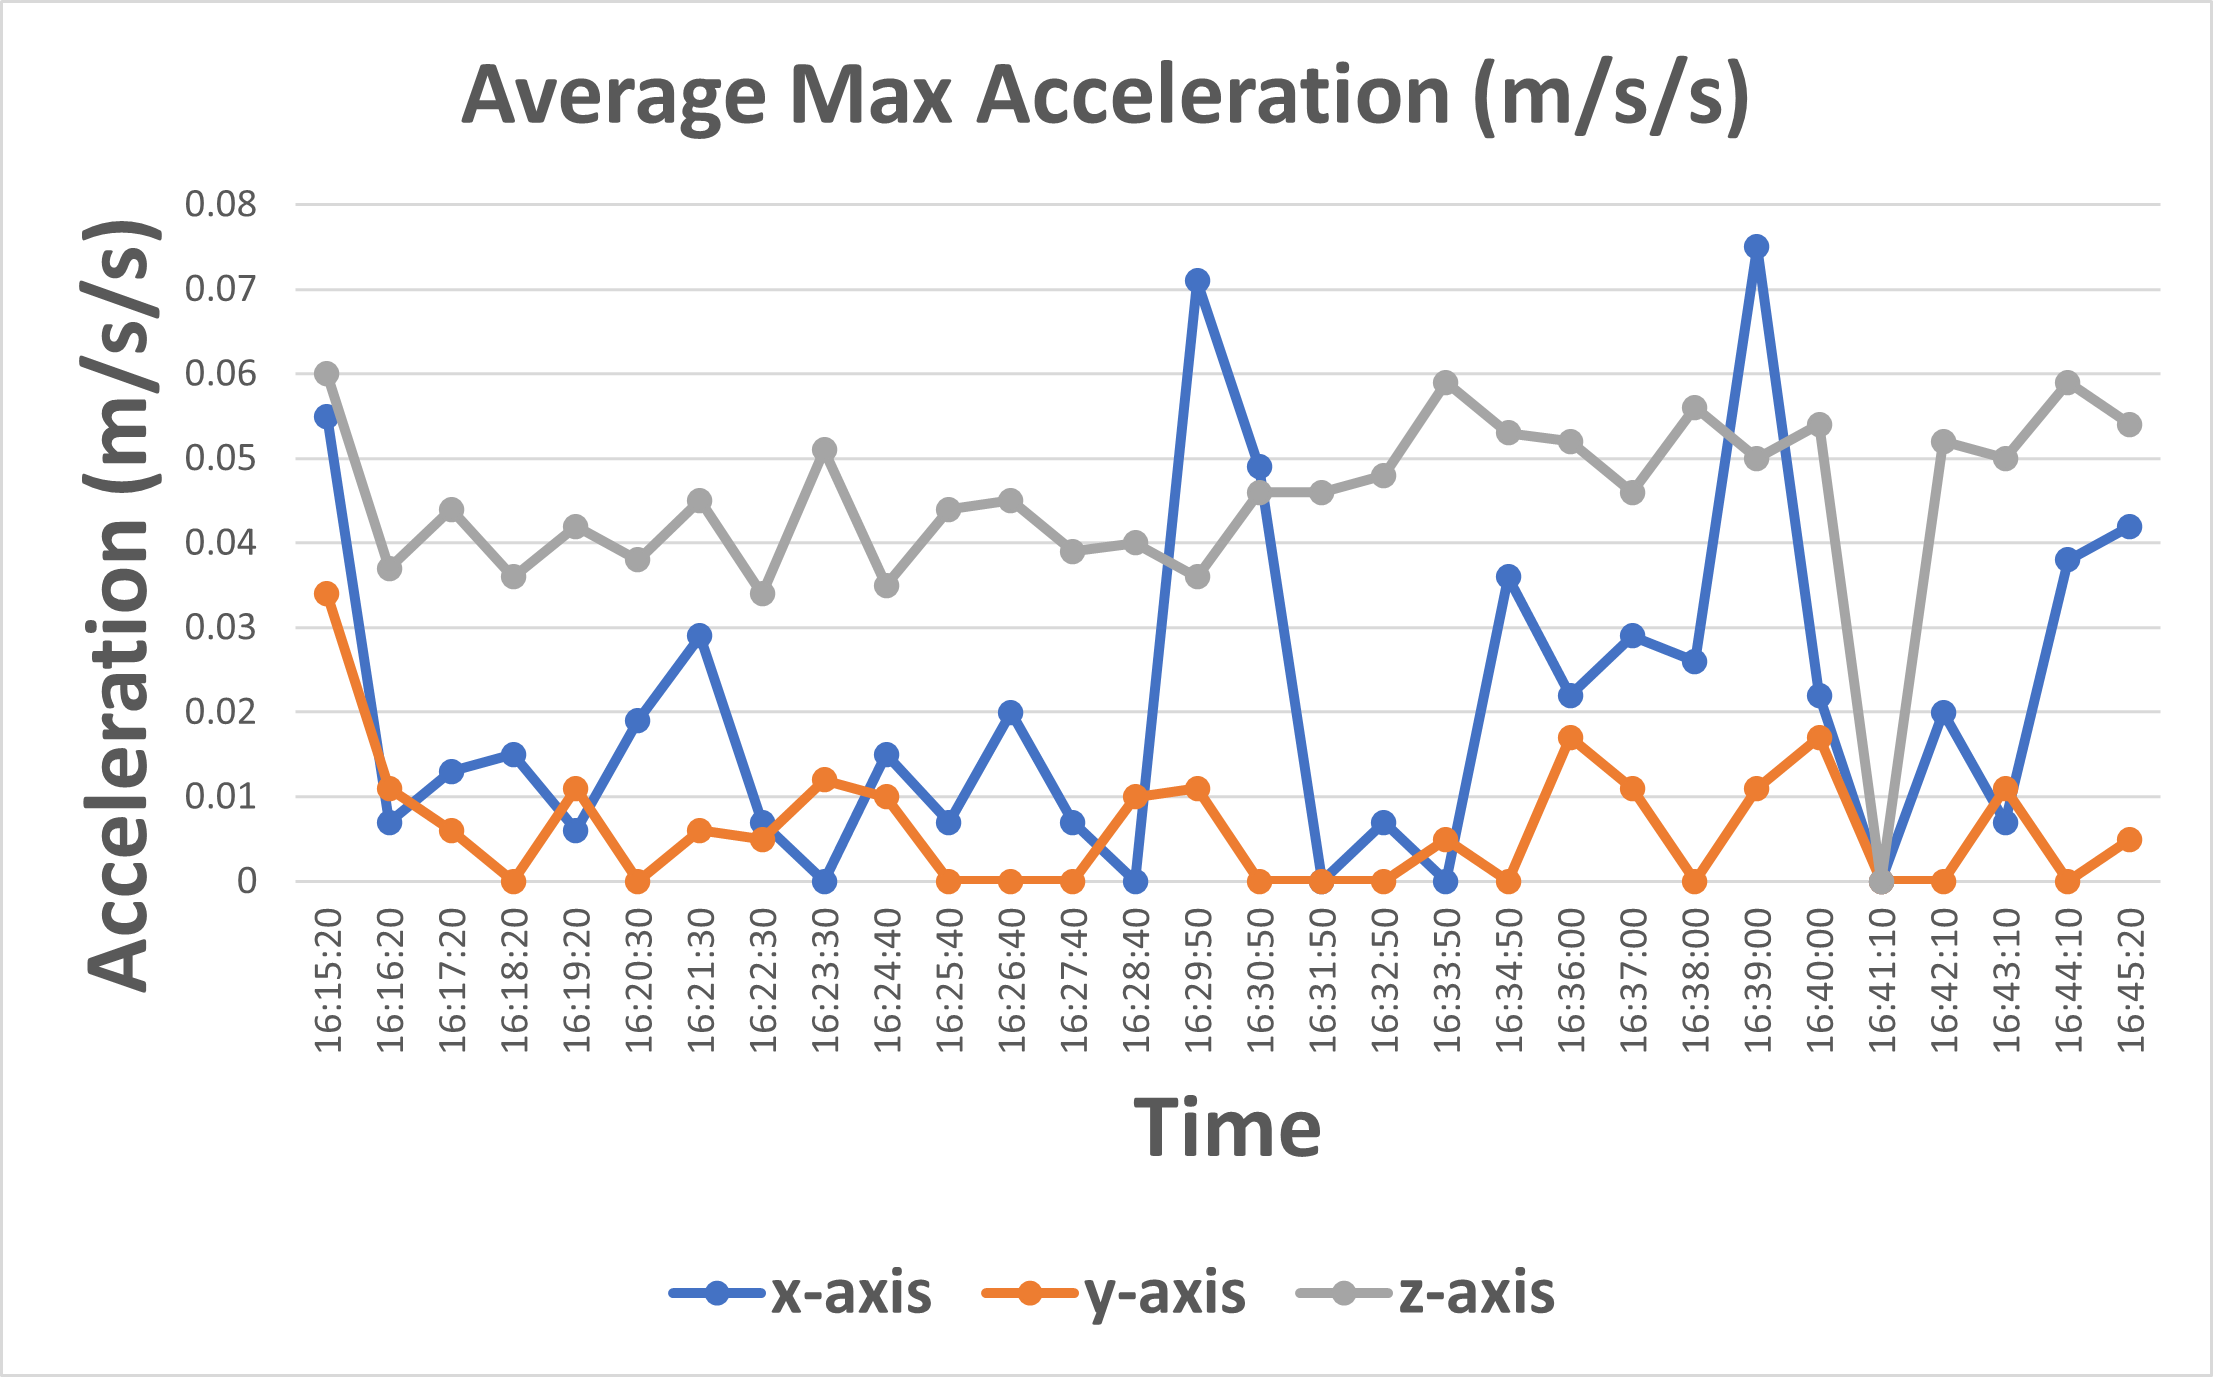
\includegraphics[width=\textwidth]{Sections/Prototype-Testing/proto2-test1-a.png}
	\label{proto2-test1-a}
\end{figure}

\begin{figure}[H]
	\centering
	\caption{Prototype 2: Test 1 Maximum Average Frequency}
	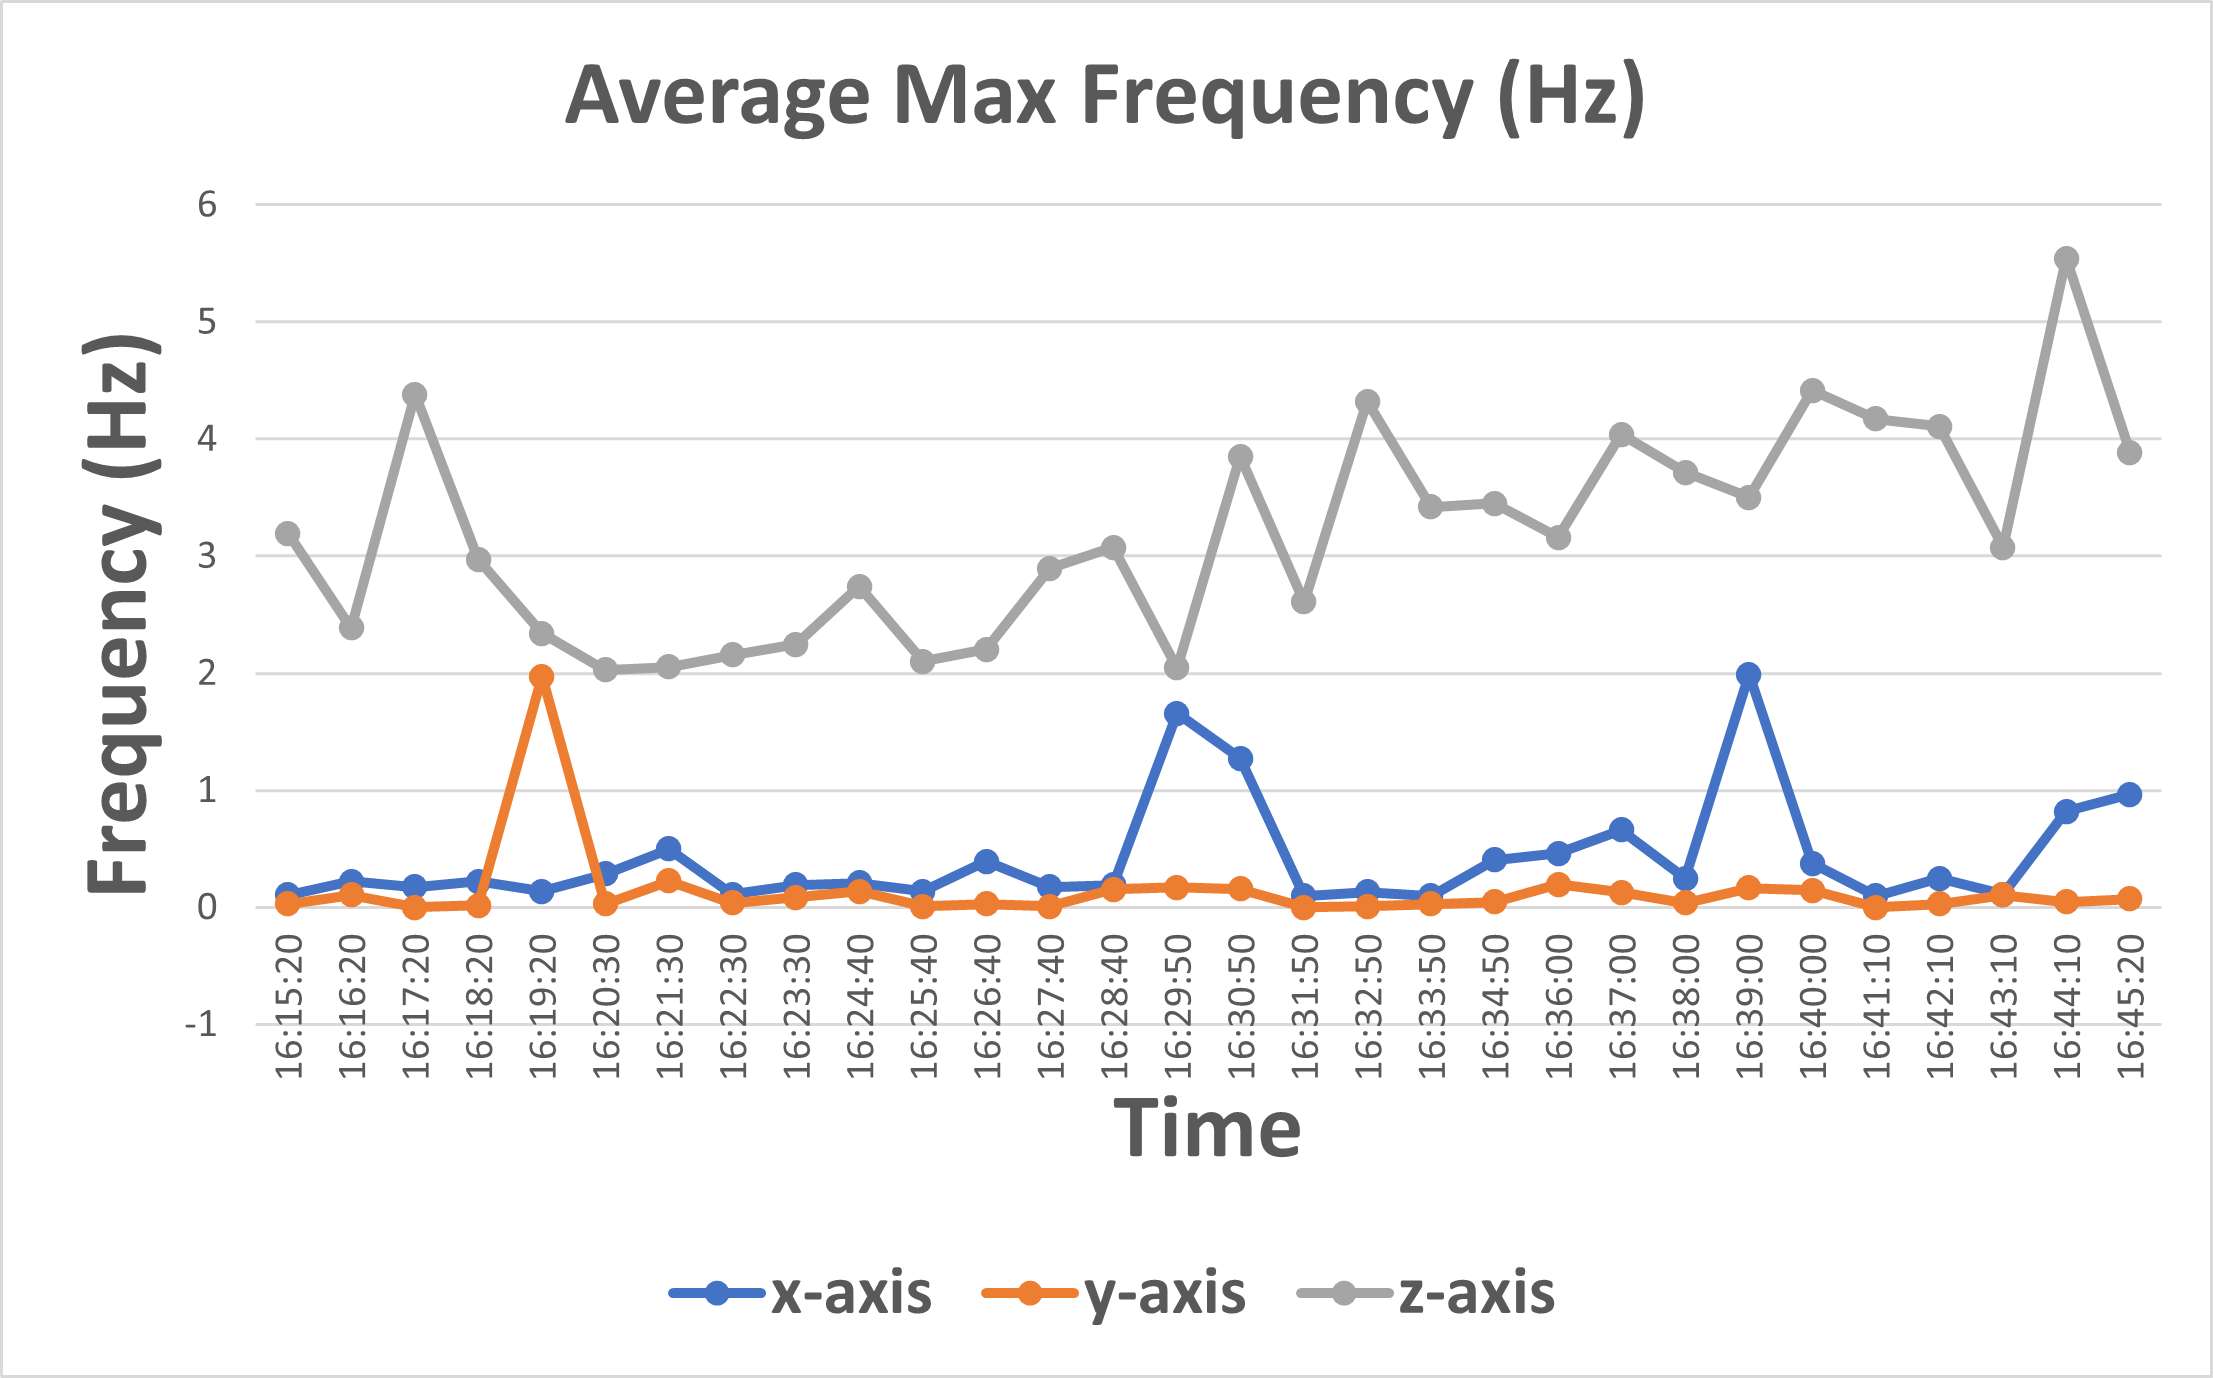
\includegraphics[width=\textwidth]{Sections/Prototype-Testing/proto2-test1-f.png}
	\label{proto2-test1-f}
\end{figure}

\begin{figure}[H]
	\centering
	\caption{Prototype 2: Test 1 SNR}
	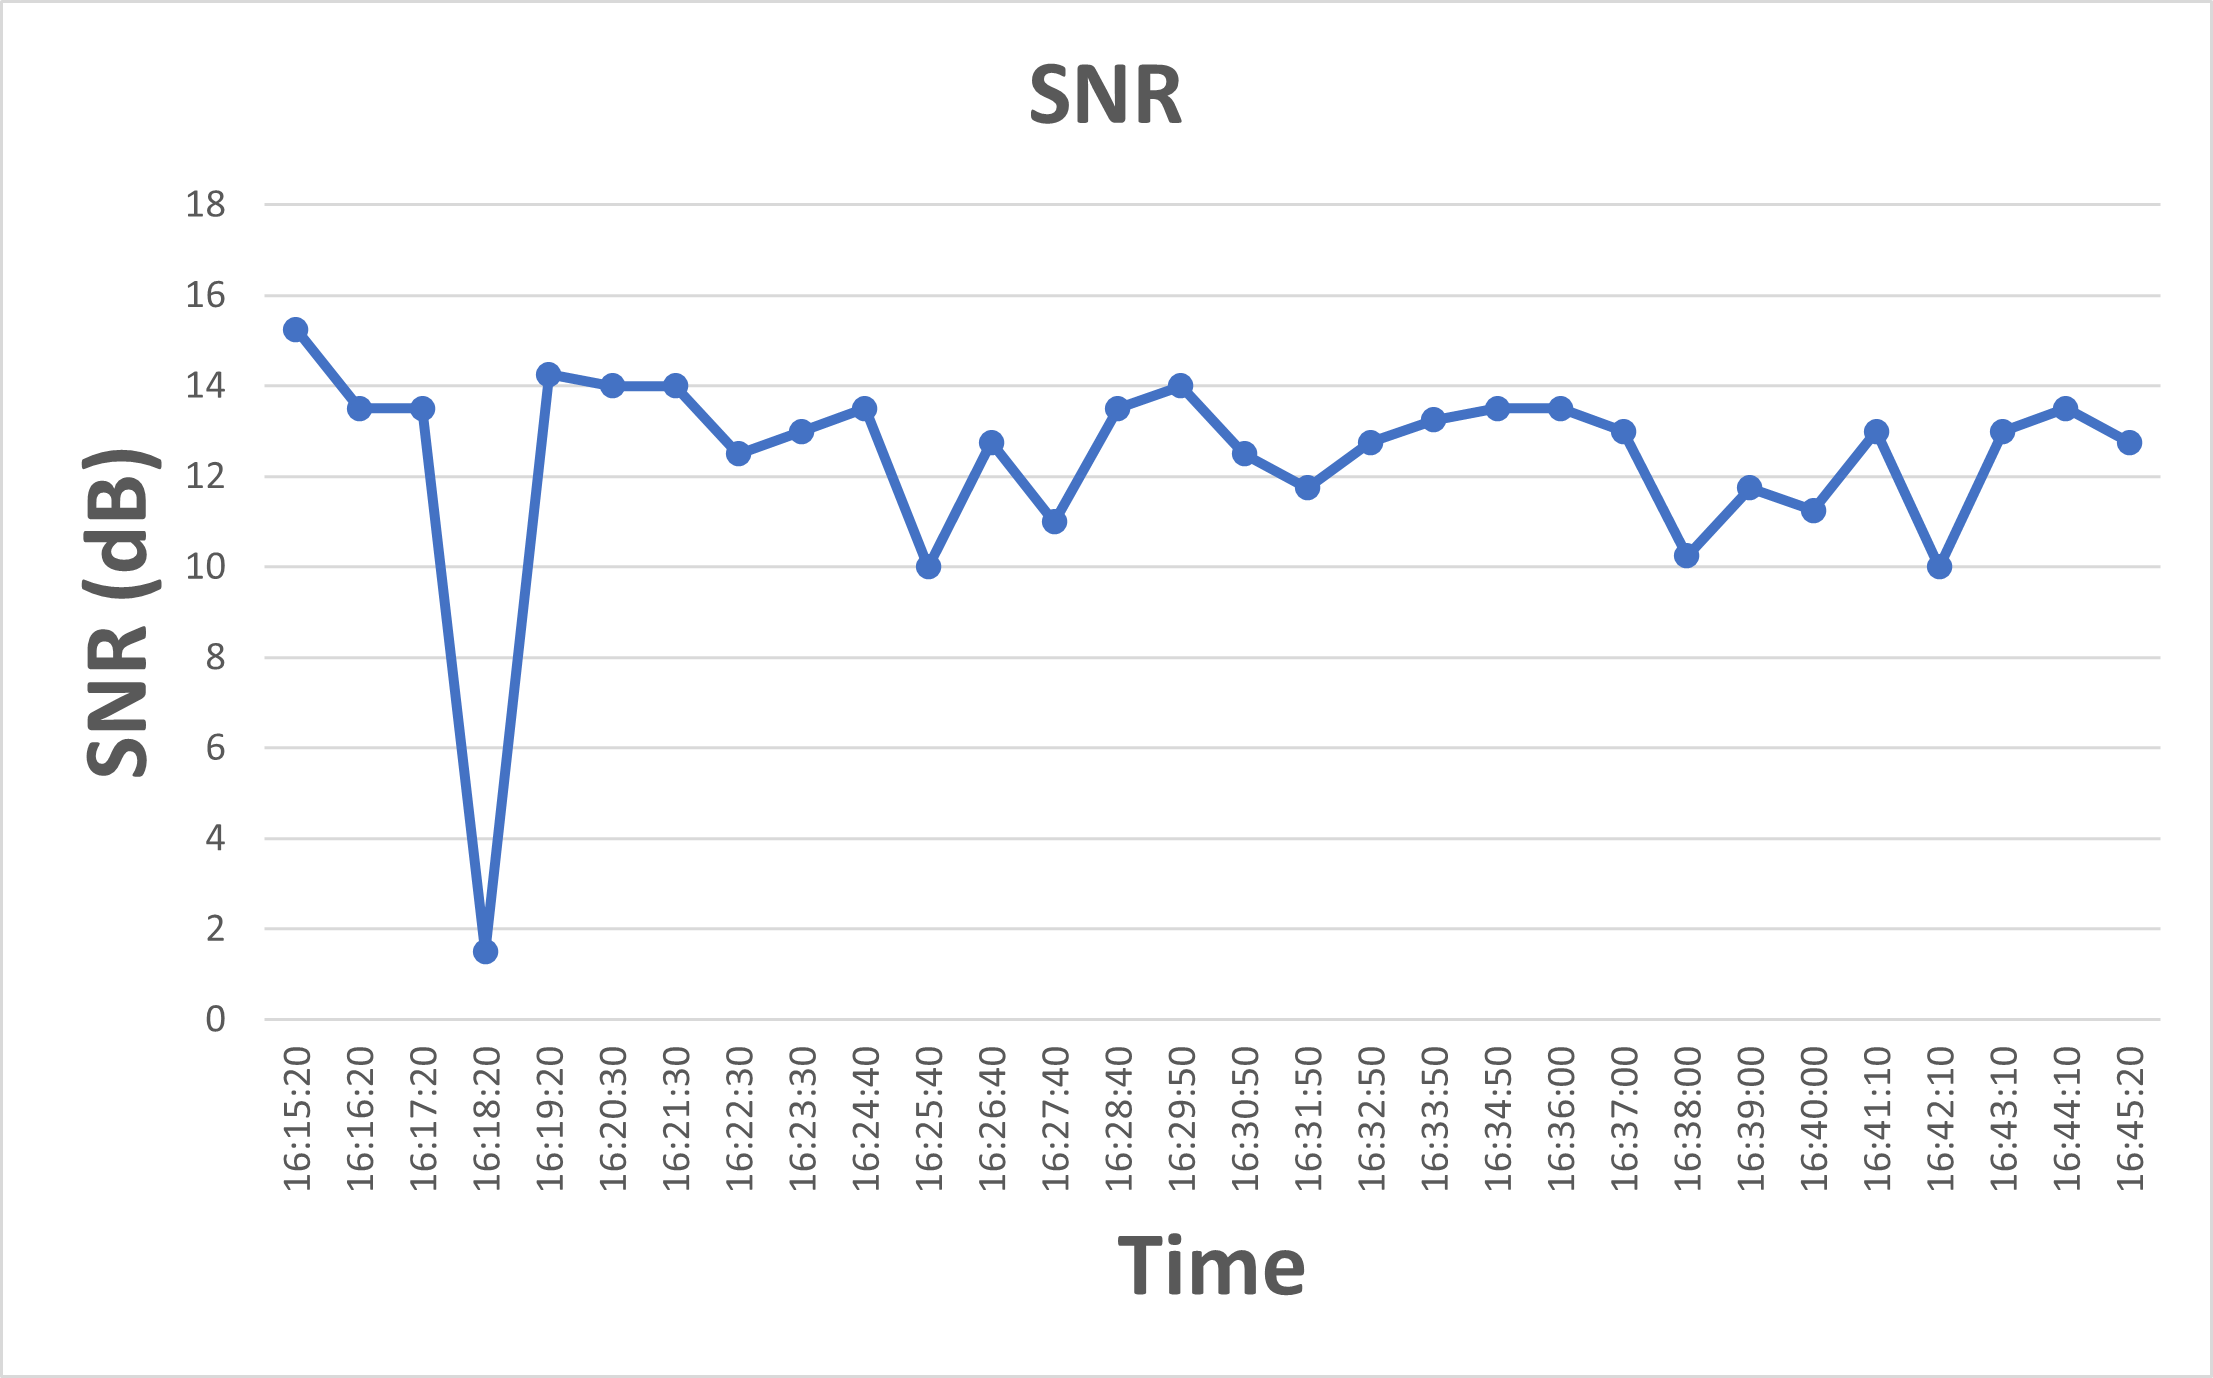
\includegraphics[width=\textwidth]{Sections/Prototype-Testing/proto2-test1-snr.png}
	\label{proto2-test1-snr}
\end{figure}

\begin{figure}[H]
	\centering
	\caption{Prototype 2: Test 1 RSSI}
	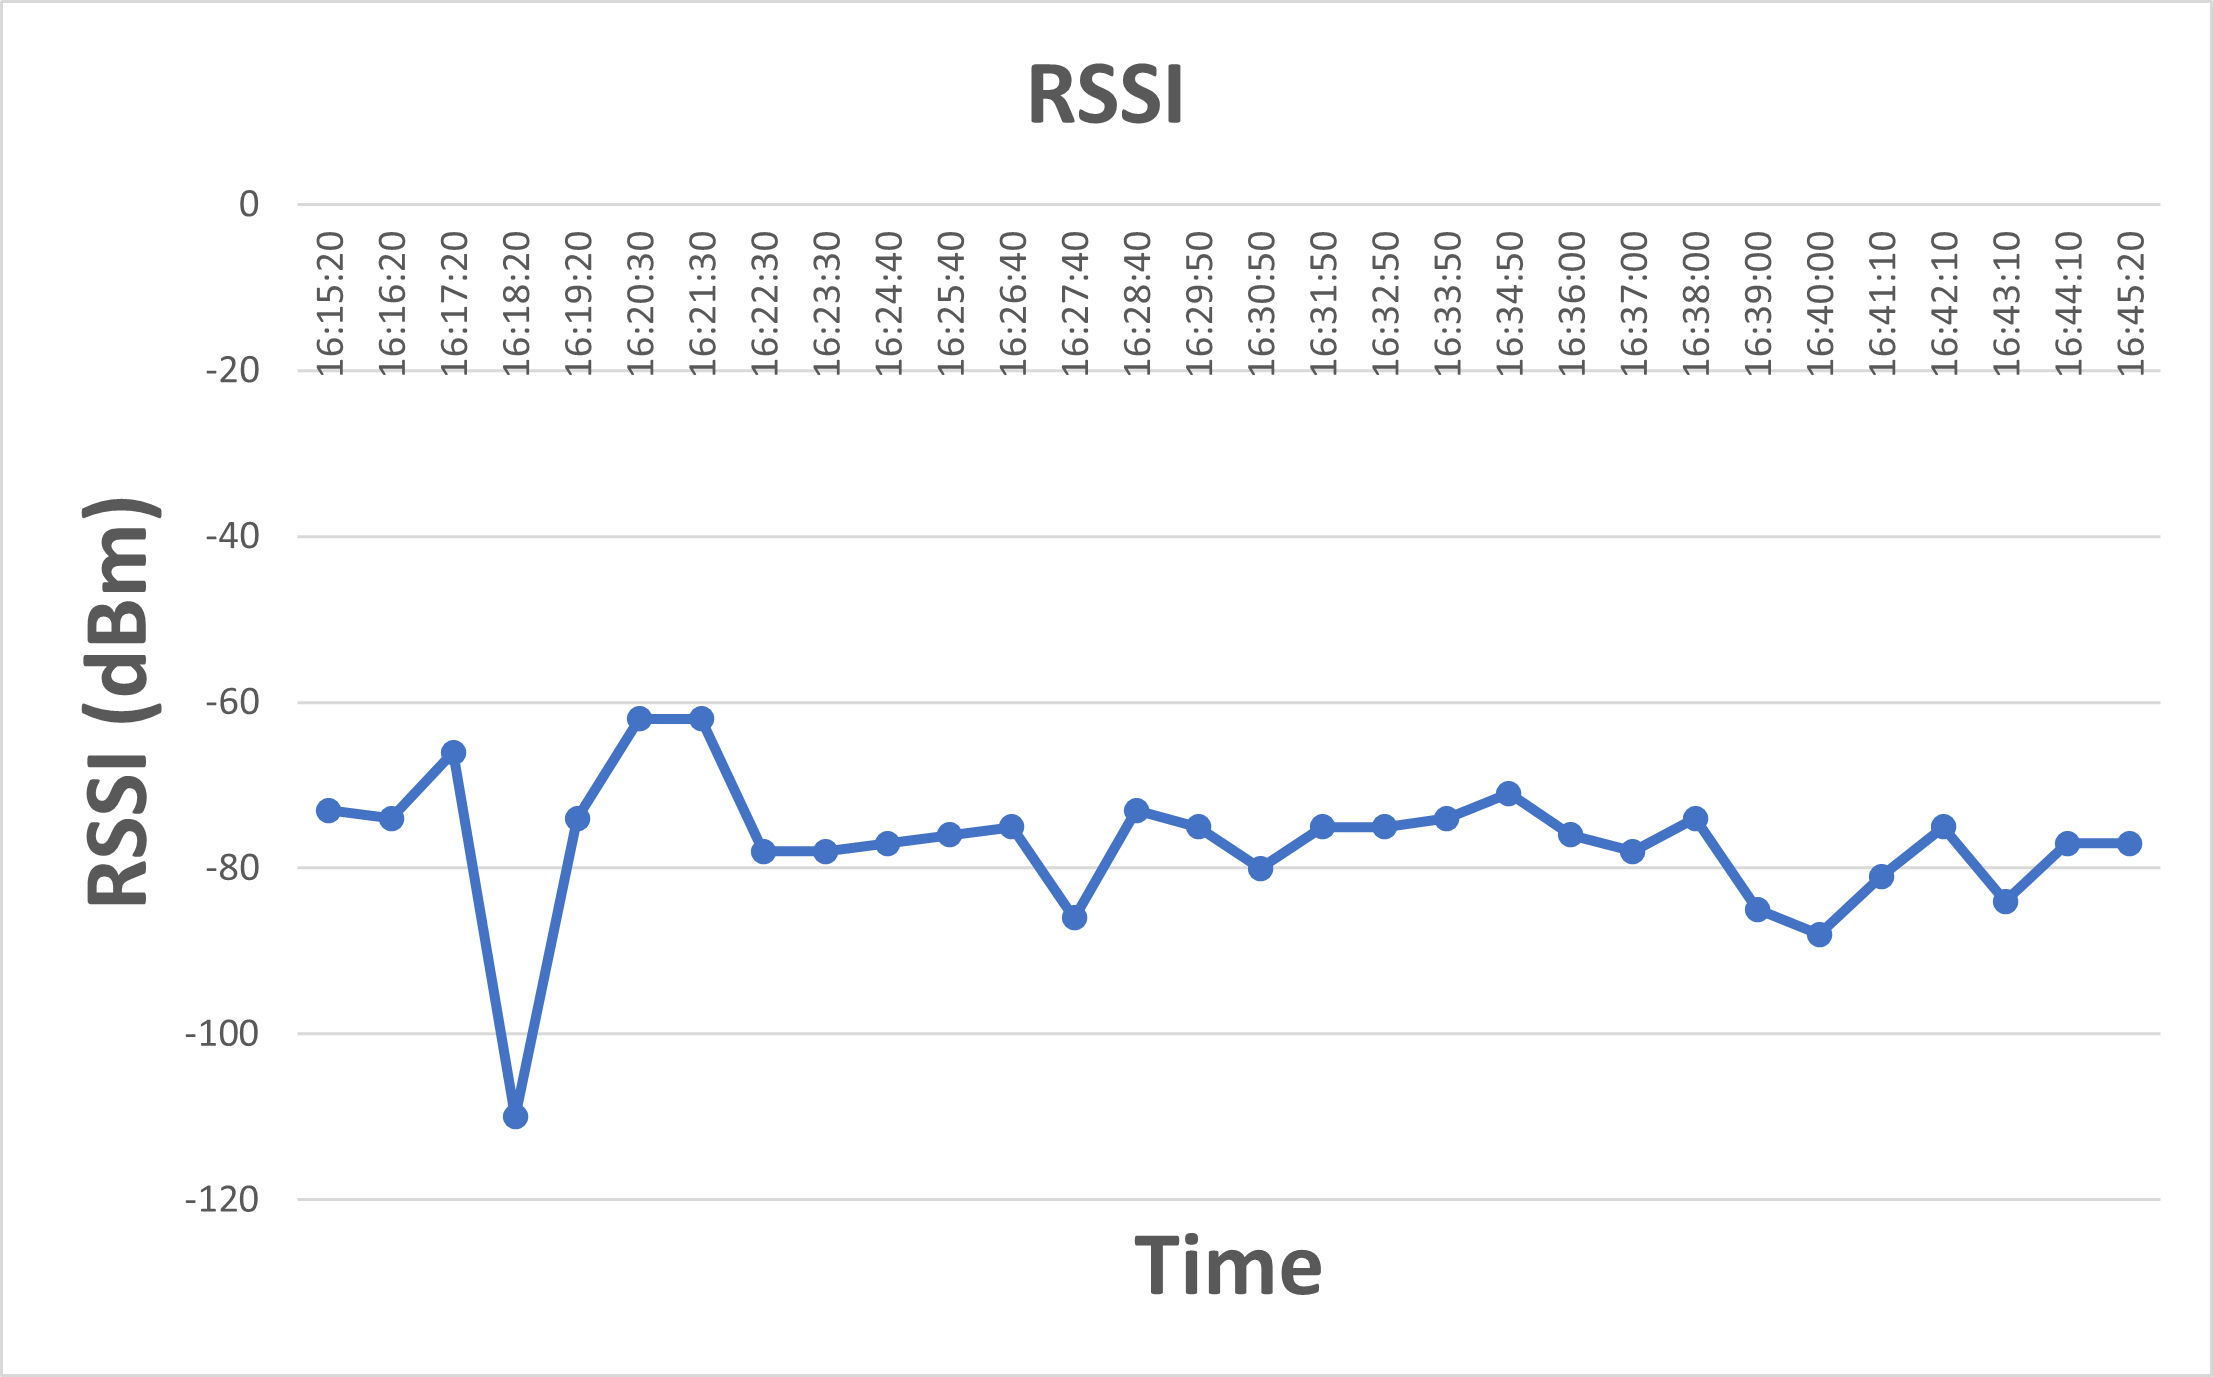
\includegraphics[width=\textwidth]{Sections/Prototype-Testing/proto2-test1-rssi.png}
	\label{proto2-test1-rssi}
\end{figure}

\subsubsection{Prototype 2: Test 2}
Test two was conducted over a thirty minute period with the same noise thresholds as test one. This time, the enclosure was removed from the rail and placed flat on the floor of the bridge. This was done to gain more context about the results from experiment one and insight for the noise threshold values used in test three. Figure \ref{bridge-ground} shows the enclosure placement for this test. Packets were again transmitted every sixty seconds and the values were observed in real time on the Arduino IoT Cloud dashboard. One participant was assigned to monitoring the incoming packets on the TNN live data page at the base station, and one to watch over the enclosure on the bridge. Special attention was required for this test since the enclosure was placed flat on the ground and was at risk of pedestrian interference. 

\begin{figure}[H]
	\centering
	\caption{Prototype 2: Test 2 Enclosure Placement}
	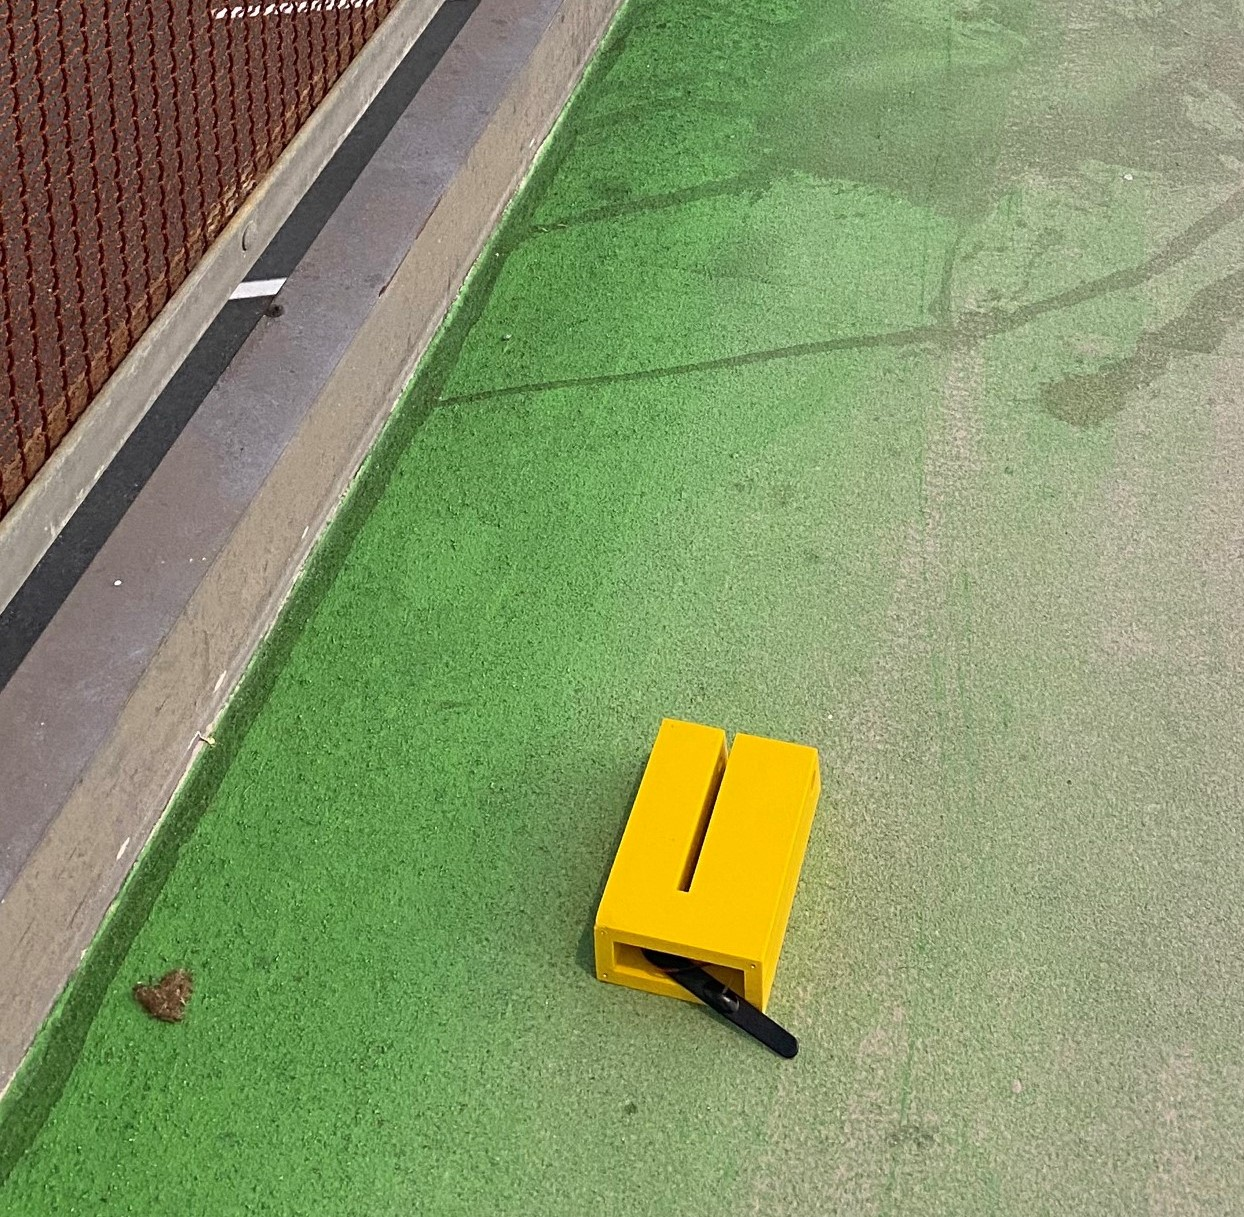
\includegraphics[width=0.8\textwidth]{Sections/Prototype-Testing/bridge-ground.png}
	\label{bridge-ground}
\end{figure}

\subsubsection{Prototype 2: Test 2 Results}
At the conclusion of test one, it was uncertain as to whether the lack of x-axis frequency was truly due to the lower noise threshold or if the z-axis was actually the result of the side of the bridge absorbing frequency components of the x-axis. To resolve this uncertainty the enclosure was placed flat on the bridge, making the z-axis representative of the vertical frequency component (test one x-axis). Since the noise thresholds were unchanged from test one, test two simultaneously tested the existence of vertical frequency components on the bridge, and the effectiveness of using a lower noise threshold for the x-axis from test one.\\\\
The z-axis displayed a frequency that was much more representative of the expected fundamental frequency of 2.2 Hz specified in the Griffith footbridge documentation \cite{griffith-bridge}. The frequency hit maximum average peaks of just over 2.5 Hz and exhibited most peaks within the 2-2.5 Hz range. The readings were also much more reactive to human induced vibrations caused by pedestrian load.\\\\
The SNR values again existed between the range of 14 dB to 10 dB which was slightly improved over test one. This can be attributed to the fact that the enclosure was lying flat on the ground with the antenna facing the direction of the base station. The RSSI was similar to test one however there was no drop below -100 dBm which was a slight improvement. Under the LoRaWAN specifications these SNR and RSSI values were characteristic of a typical LoRa signal strength. 

\begin{figure}[H]
	\centering
	\caption{Prototype 2: Test 2 Maximum Average Acceleration}
	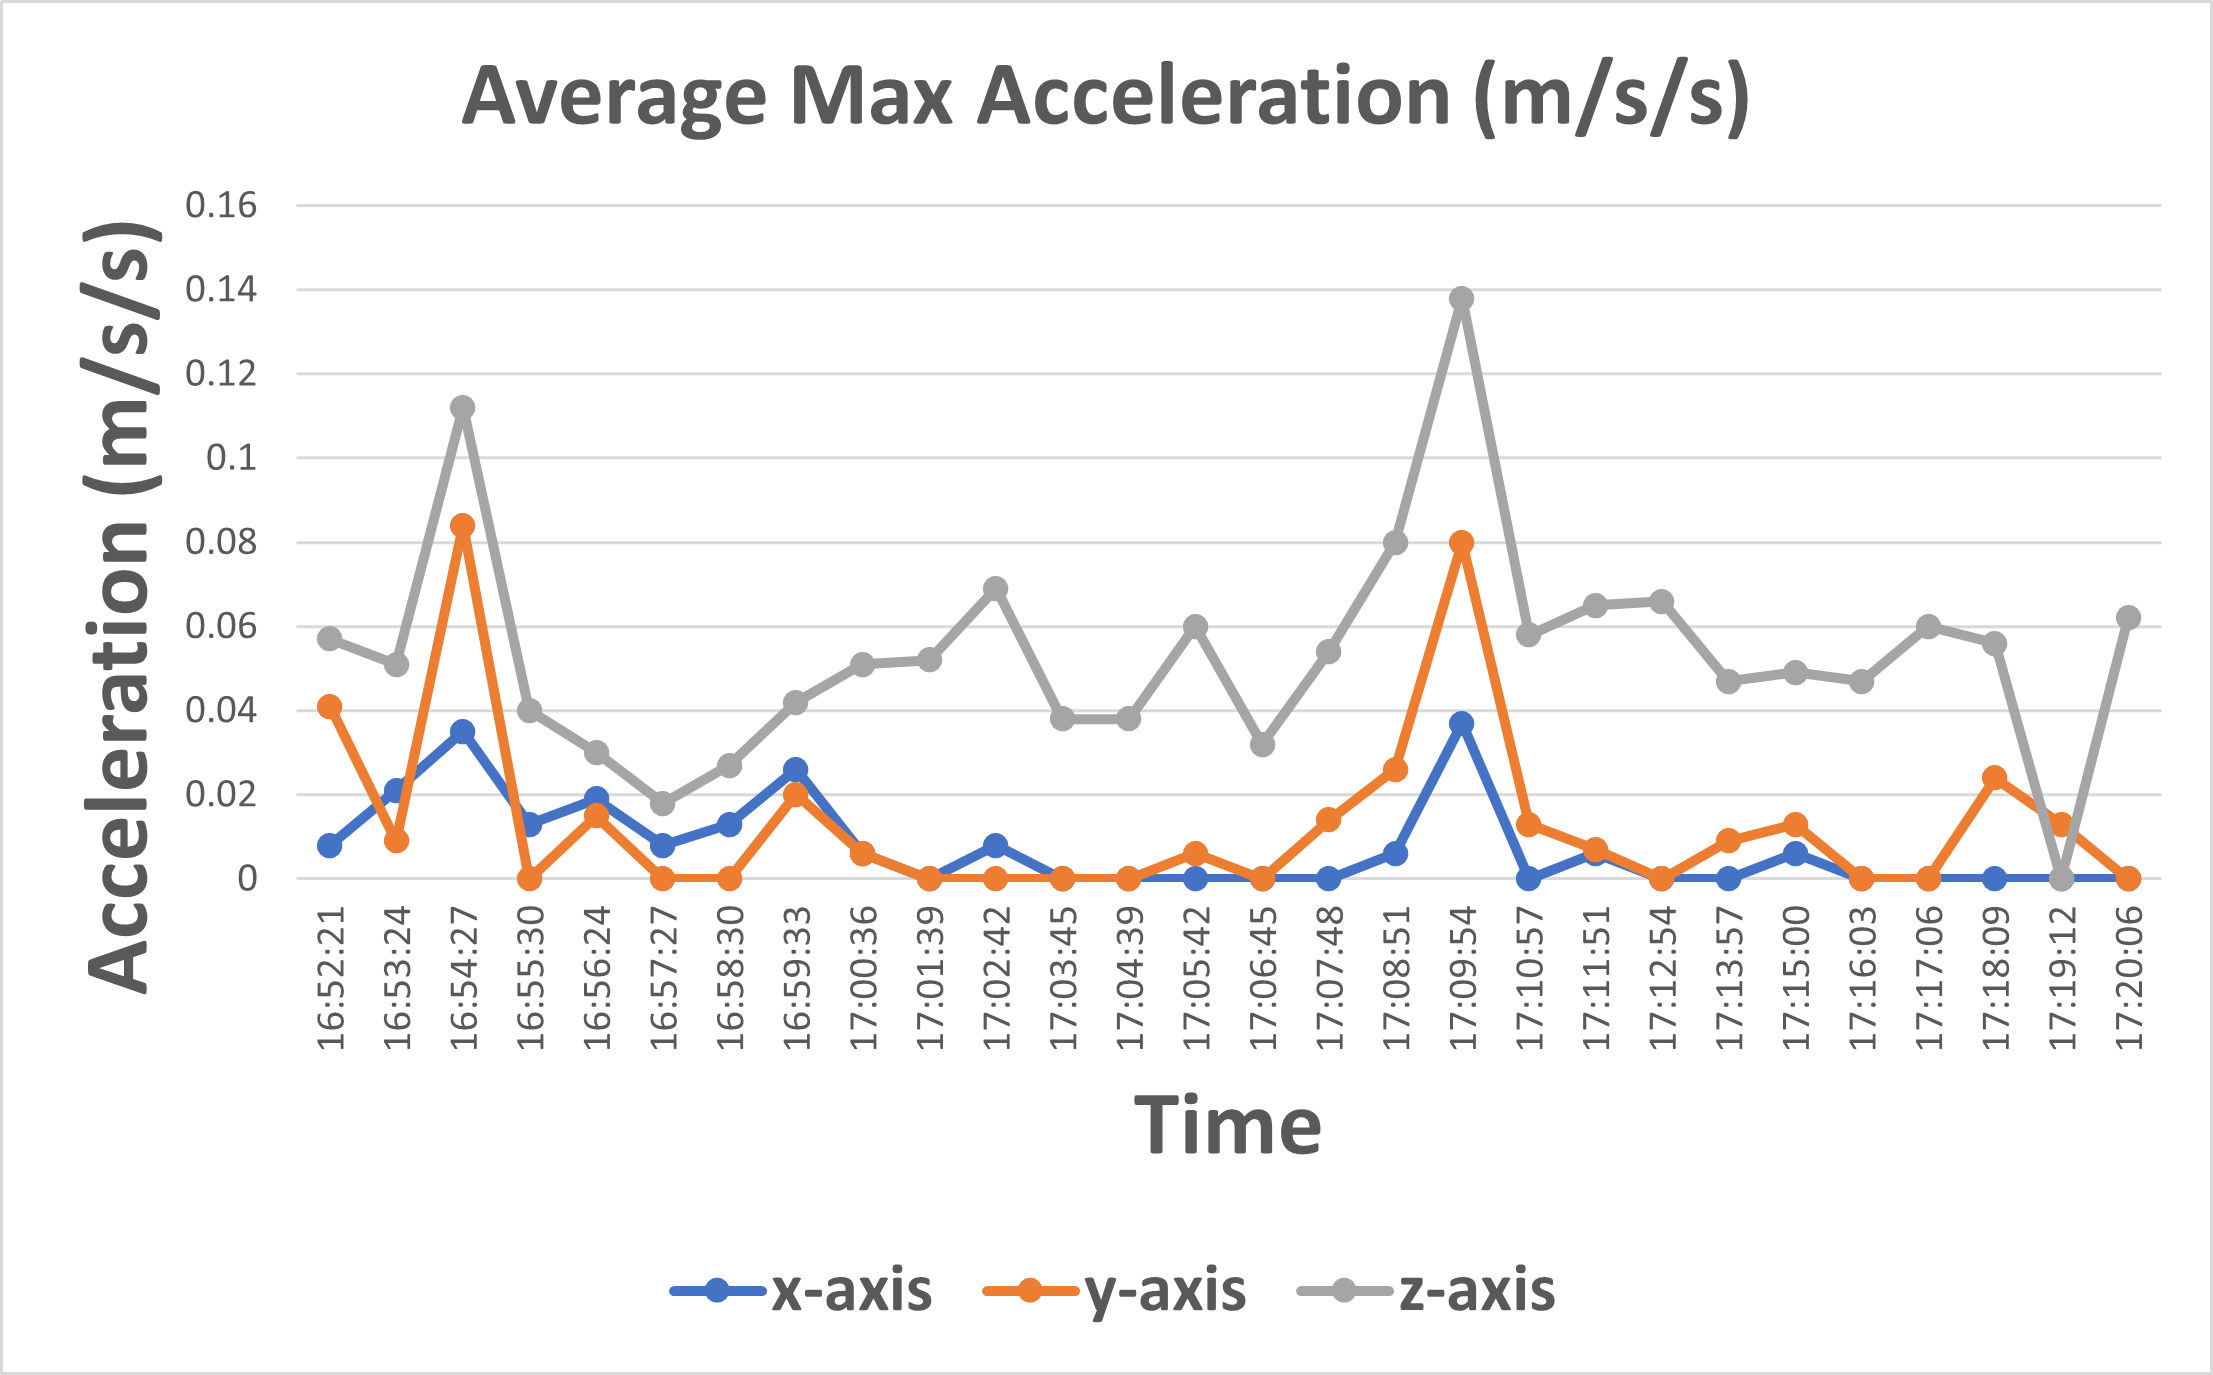
\includegraphics[width=\textwidth]{Sections/Prototype-Testing/proto2-test2-a.png}
	\label{proto2-test2-a}
\end{figure}

\begin{figure}[H]
	\centering
	\caption{Prototype 2: Test 2 Maximum Average Frequency}
	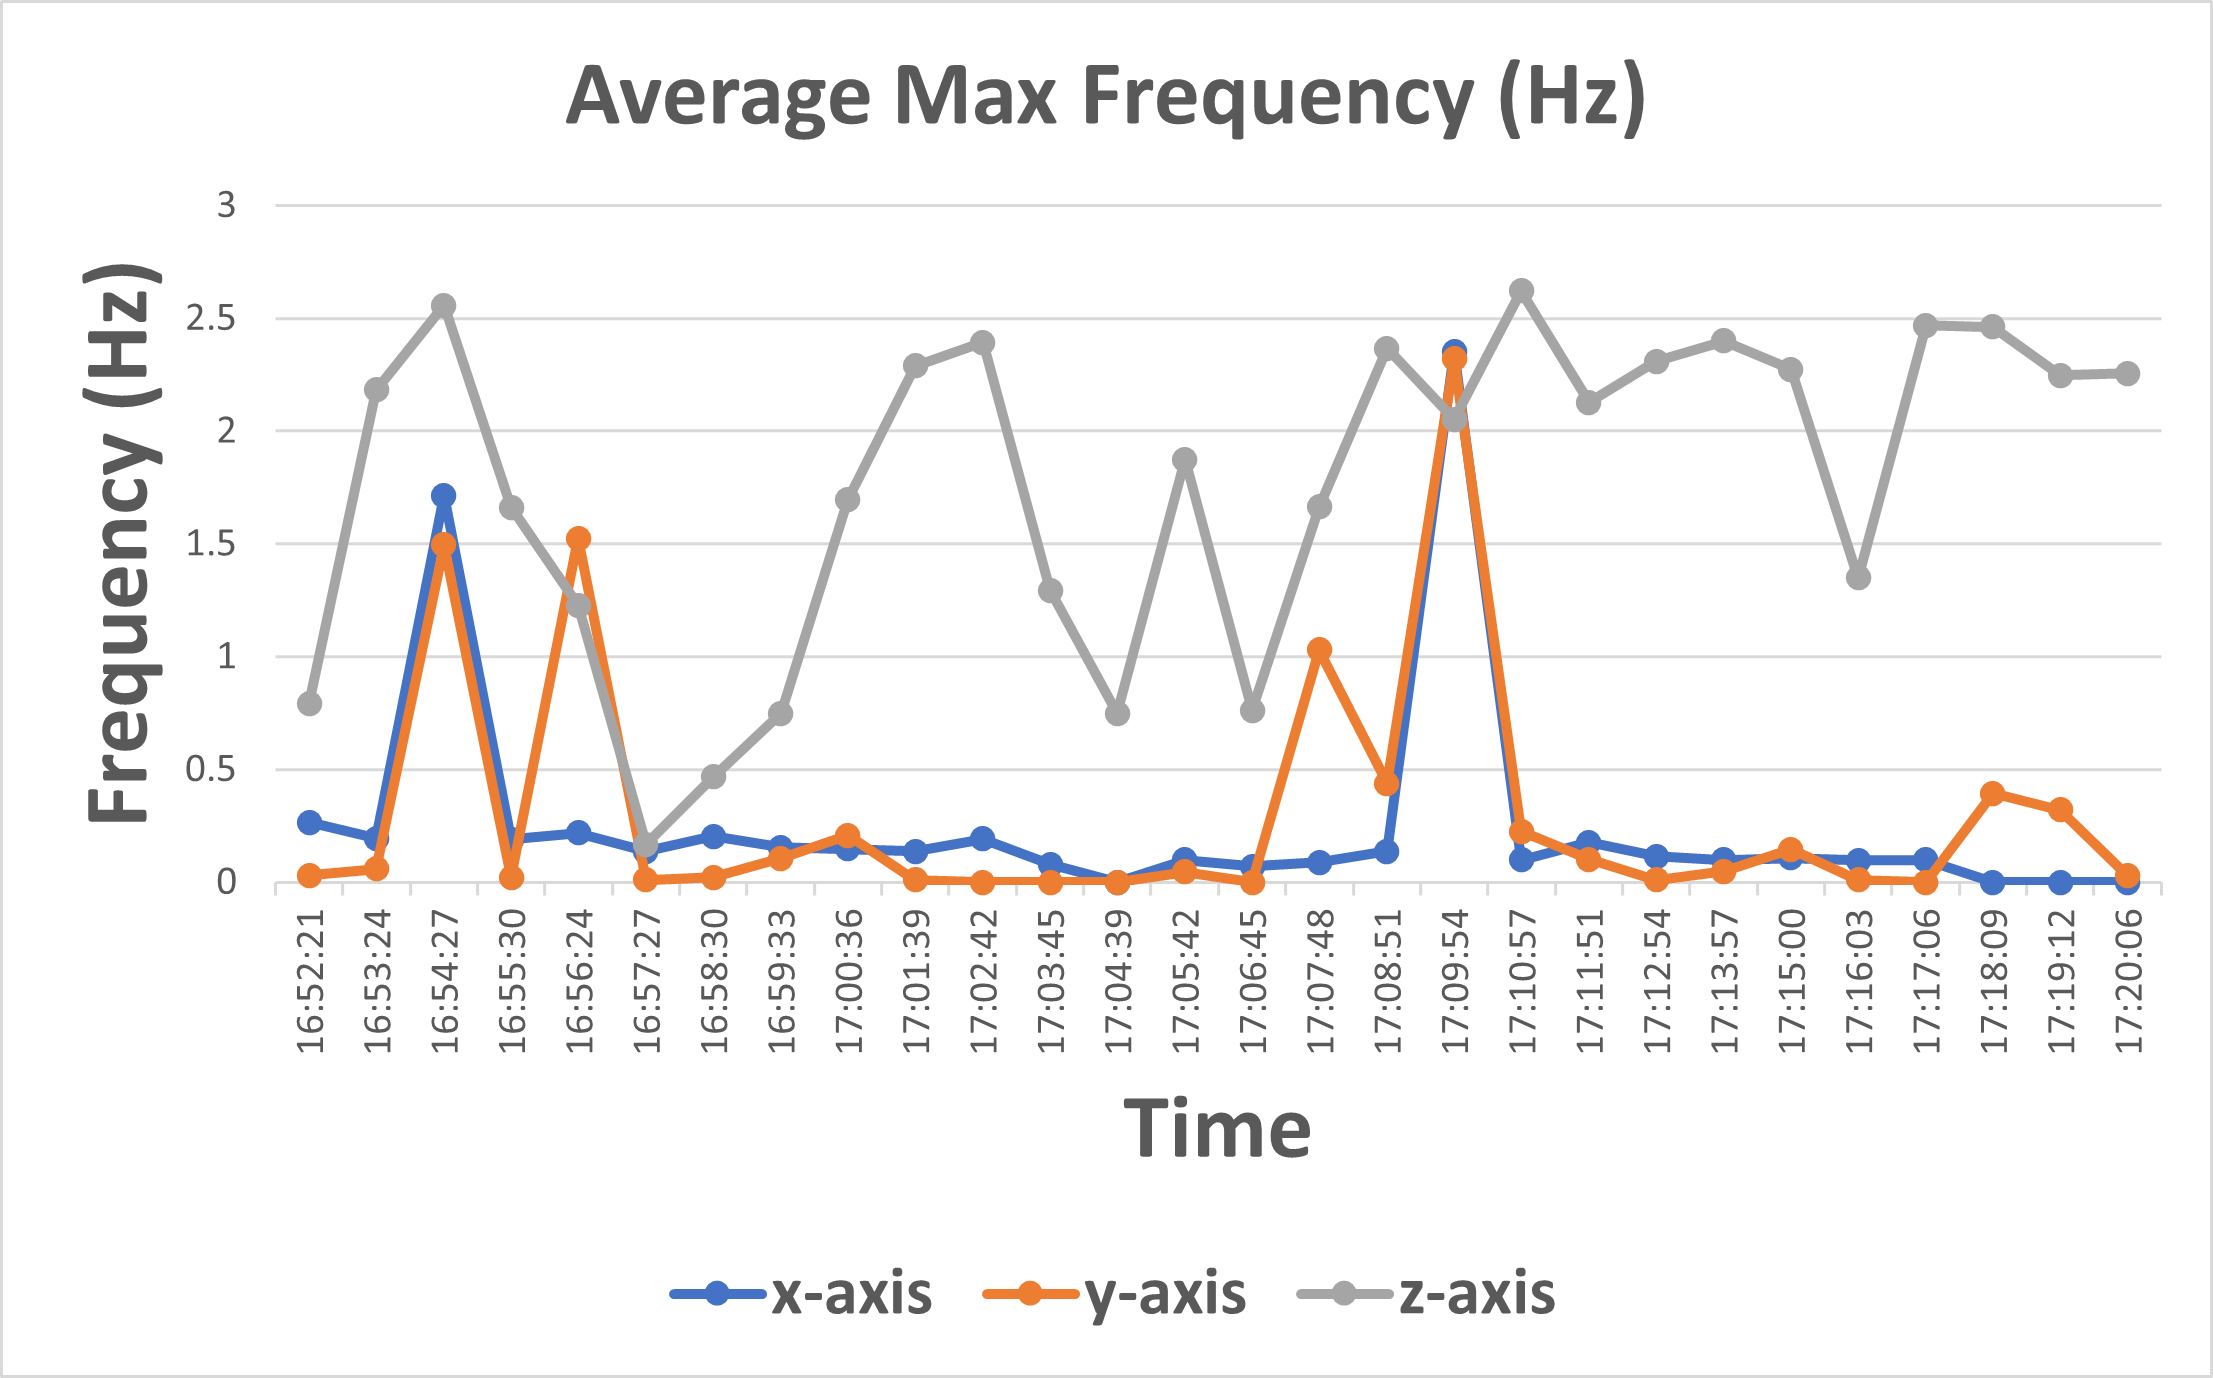
\includegraphics[width=\textwidth]{Sections/Prototype-Testing/proto2-test2-f.png}
	\label{proto2-test2-f}
\end{figure}

\begin{figure}[H]
	\centering
	\caption{Prototype 2: Test 2 SNR}
	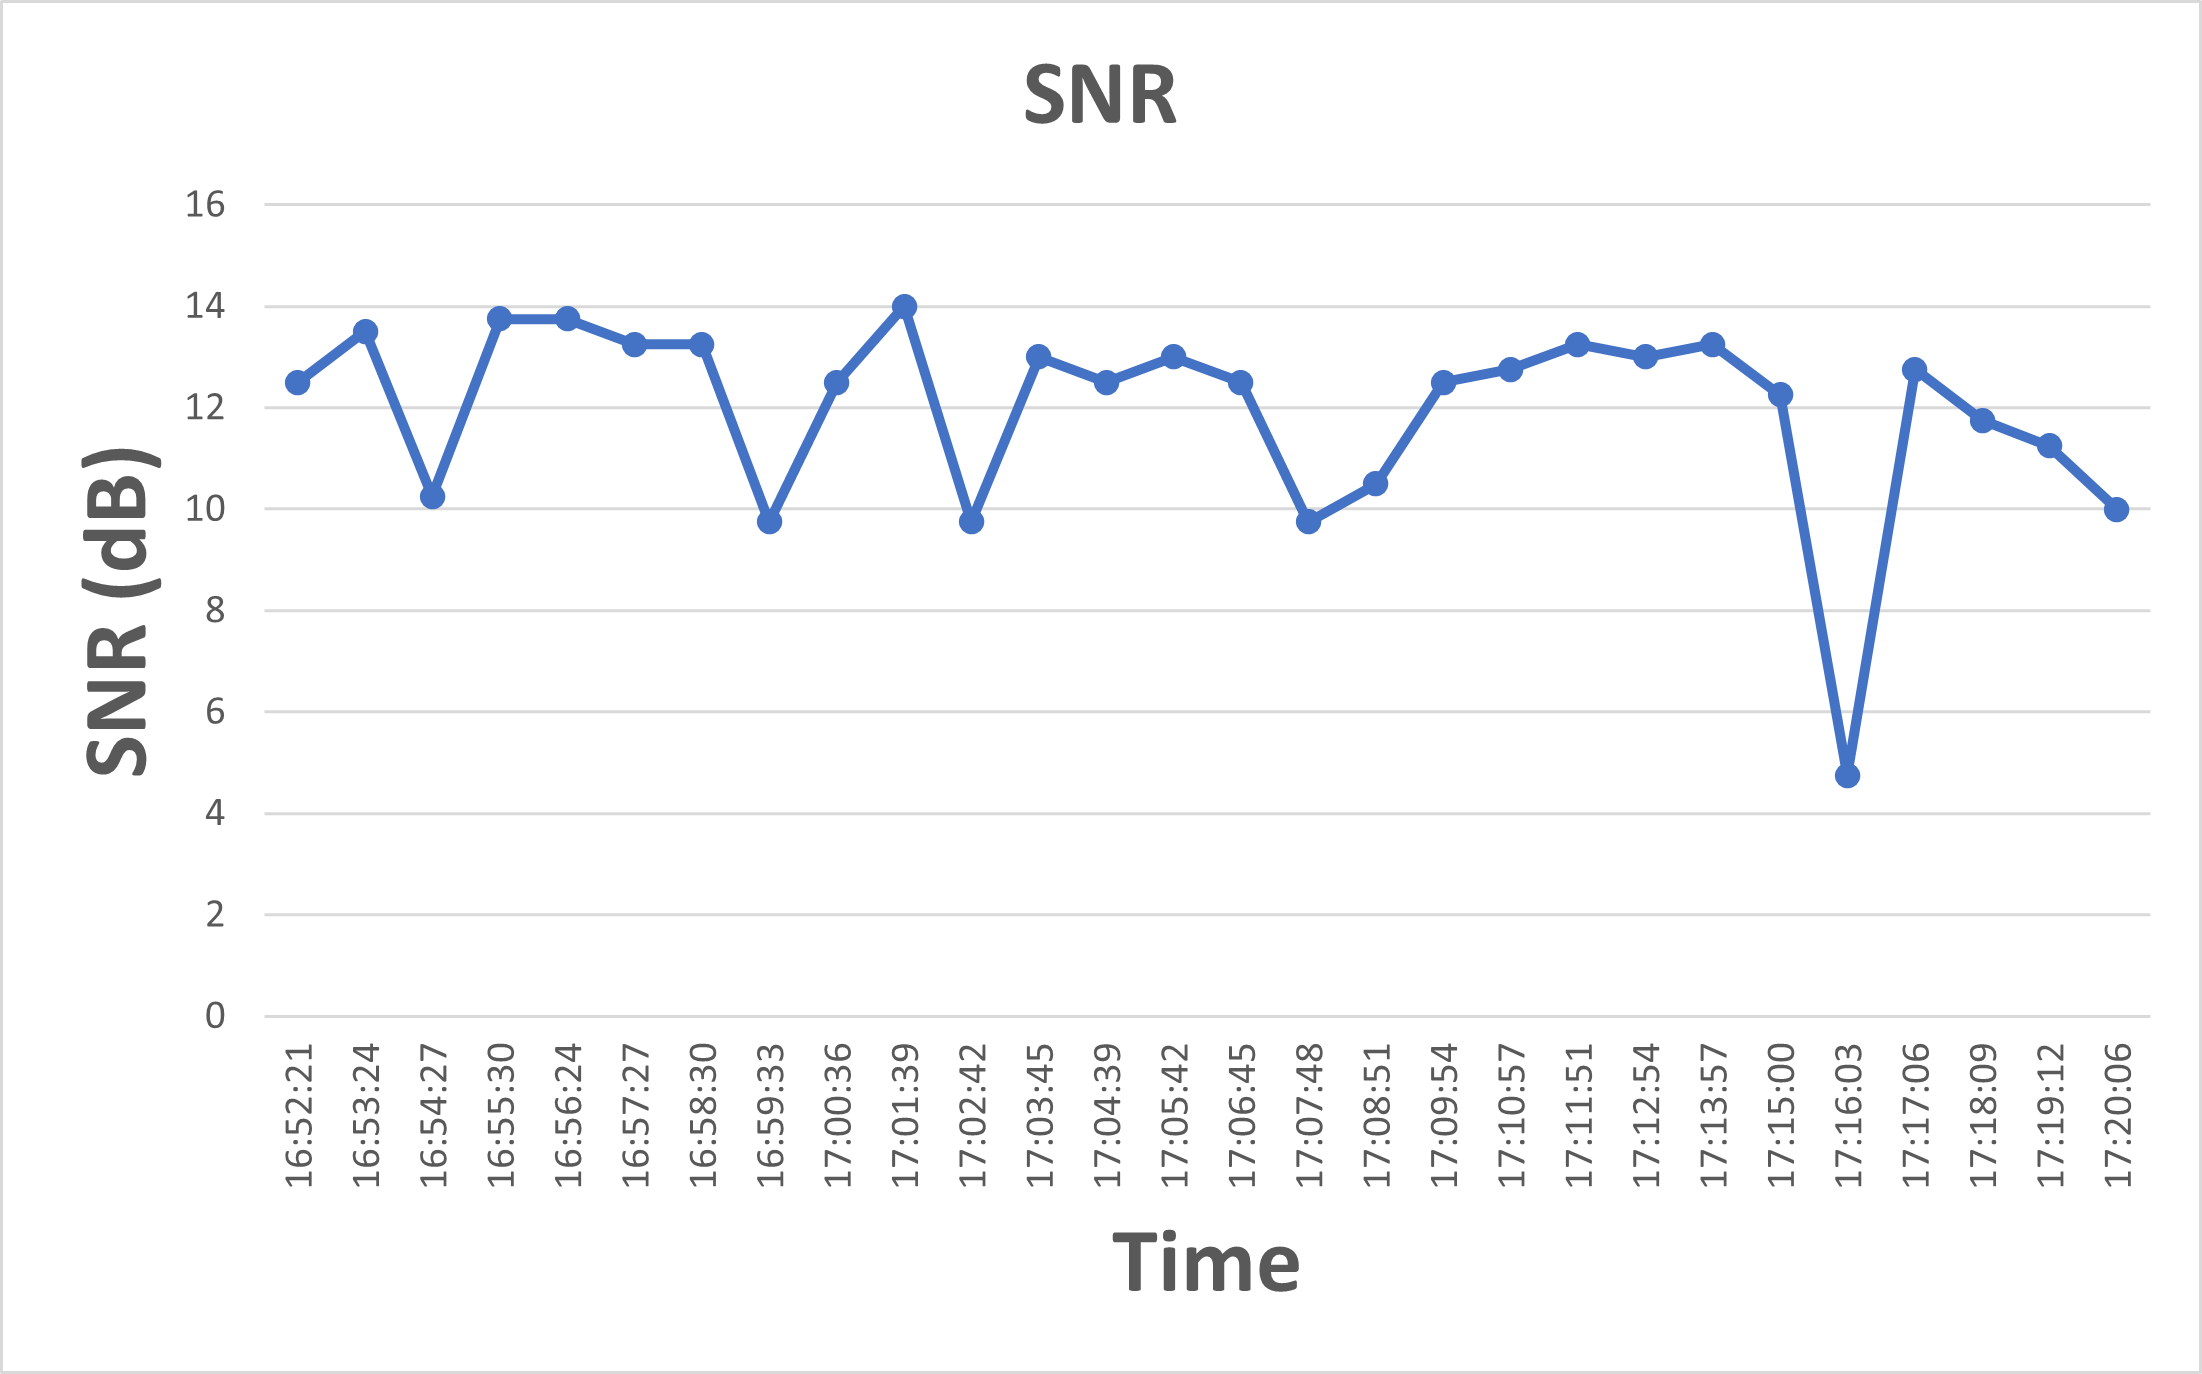
\includegraphics[width=\textwidth]{Sections/Prototype-Testing/proto2-test2-snr.png}
	\label{proto2-test2-snr}
\end{figure}

\begin{figure}[H]
	\centering
	\caption{Prototype 2: Test 2 RSSI}
	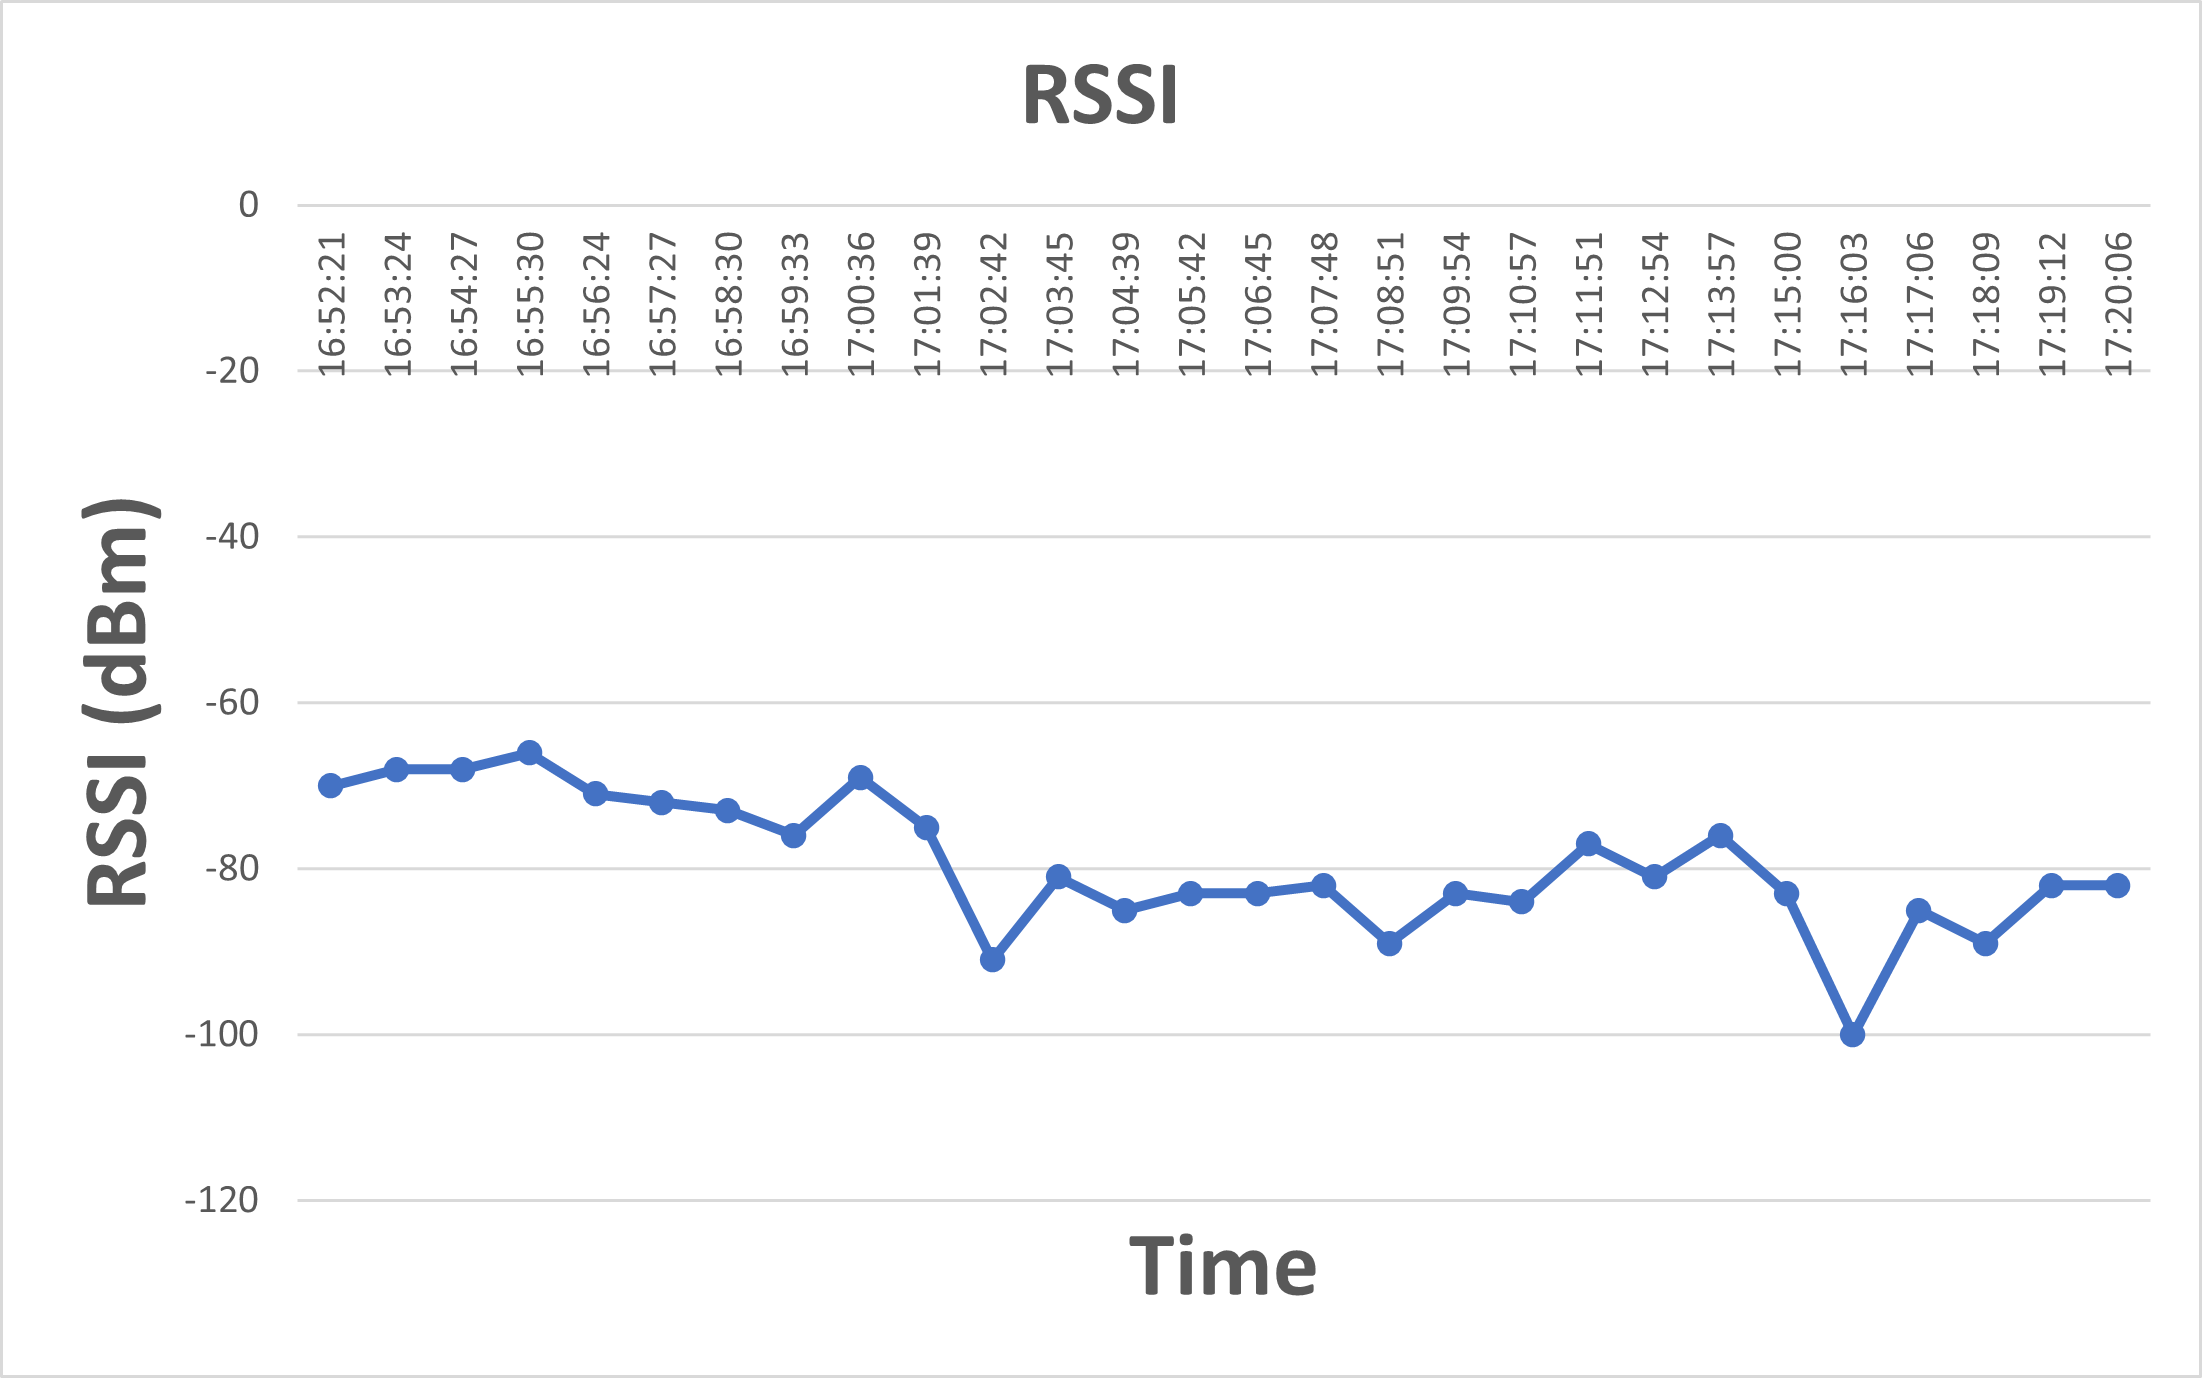
\includegraphics[width=\textwidth]{Sections/Prototype-Testing/proto2-test2-rssi.png}
	\label{proto2-test2-rssi}
\end{figure}

\subsubsection{Prototype 2: Test 3}
Test three was also conducted over a thirty minute period and the enclosure was reinstalled onto the bridge handrail. In this test the noise thresholds were changed to 0.03 for each axis. Packets were transmitted every sixty seconds and each participant fulfilled the same roles specified in test one and two. 
\begin{comment}
\section{Test Results}
\subsection{Prototype 1: Beam Test Reults}
\subsection{Prototype 2: Bridge Test Results}
\end{comment}




\subsubsection{Prototype 2: Test 3 Results}
Test three was conducted with decreased noise thresholds of 0.03 for each axis. Compared to test one, there was a significantly improved response in the x-axis with an average maximum frequency value of 2.5 Hz. This value is also more stable compared to the previous tests with peak frequencies lying between 2 Hz and 3.5 Hz whilst showing the response characteristics of increased vibration from pedestrian load due to the resonance phenomenon. With the insight from all three experiments, it is clear that a noise threshold value of 0.03 for the x-axis was much more representative of the expected 2.2 Hz for the first mode flexural frequency of the bridge. It is also apparent that 0.03 is too low for the other axis as there are elements of cross talk and noise in the y-axis and z-axis frequency response. The noise thresholds for these axis need to be increased to become more representative of the bridge's y-axis and z-axis frequency components.\\\\
In terms of SNR and RSSI, similar values from test one and two were achieved. There was a a -5 dB drop in SNR and -120 dBm drop in RSSI during this test which was the lowest signal drop in all three experiments. It is clear that the direction of the antenna plays a role in the signal strength as tests one and two involve the antenna facing upwards. Regardless of the drop, the resilient nature of LoRaWAN means that the packet was not completely dropped and the signal was able to resume normal functionality. Notably, this drop occurred at 17:43:40 which corresponds to a strong peak in the average max acceleration. This peak may therefore be attributed to noise or corruption and may not be indicative of the bridge's actual acceleration response. 

\begin{figure}[H]
	\centering
	\caption{Prototype 2: Test 3 Maximum Average Acceleration}
	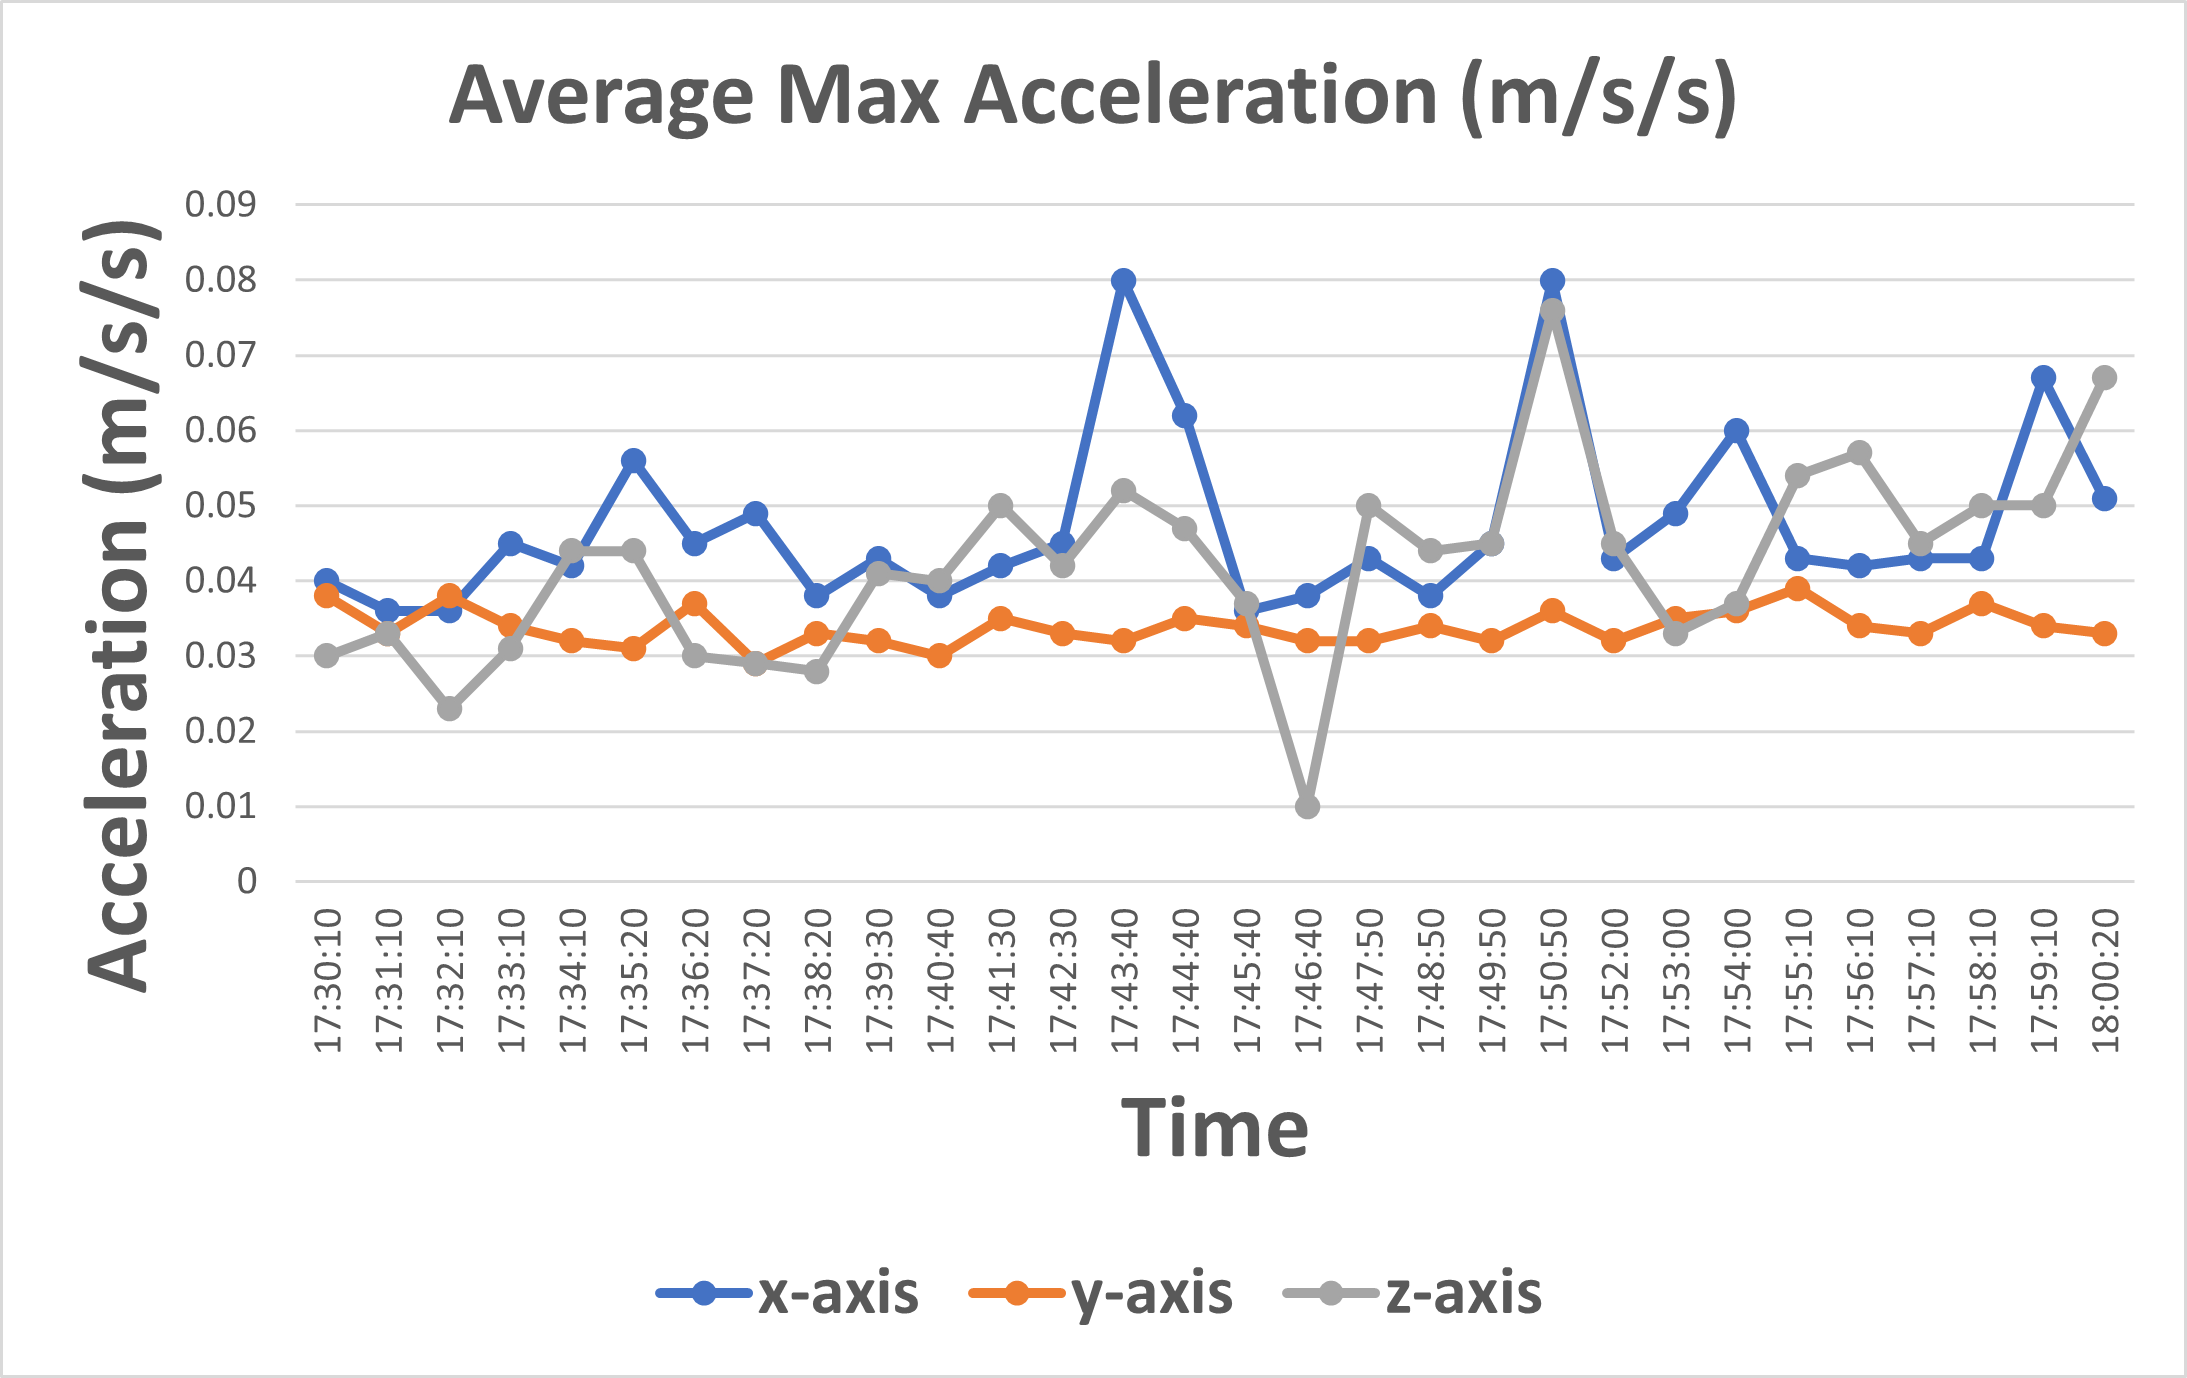
\includegraphics[width=\textwidth]{Sections/Prototype-Testing/proto2-test3-a.png}
	\label{proto2-test3-a}
\end{figure}

\begin{figure}[H]
	\centering
	\caption{Prototype 2: Test 3 Maximum Average Frequency}
	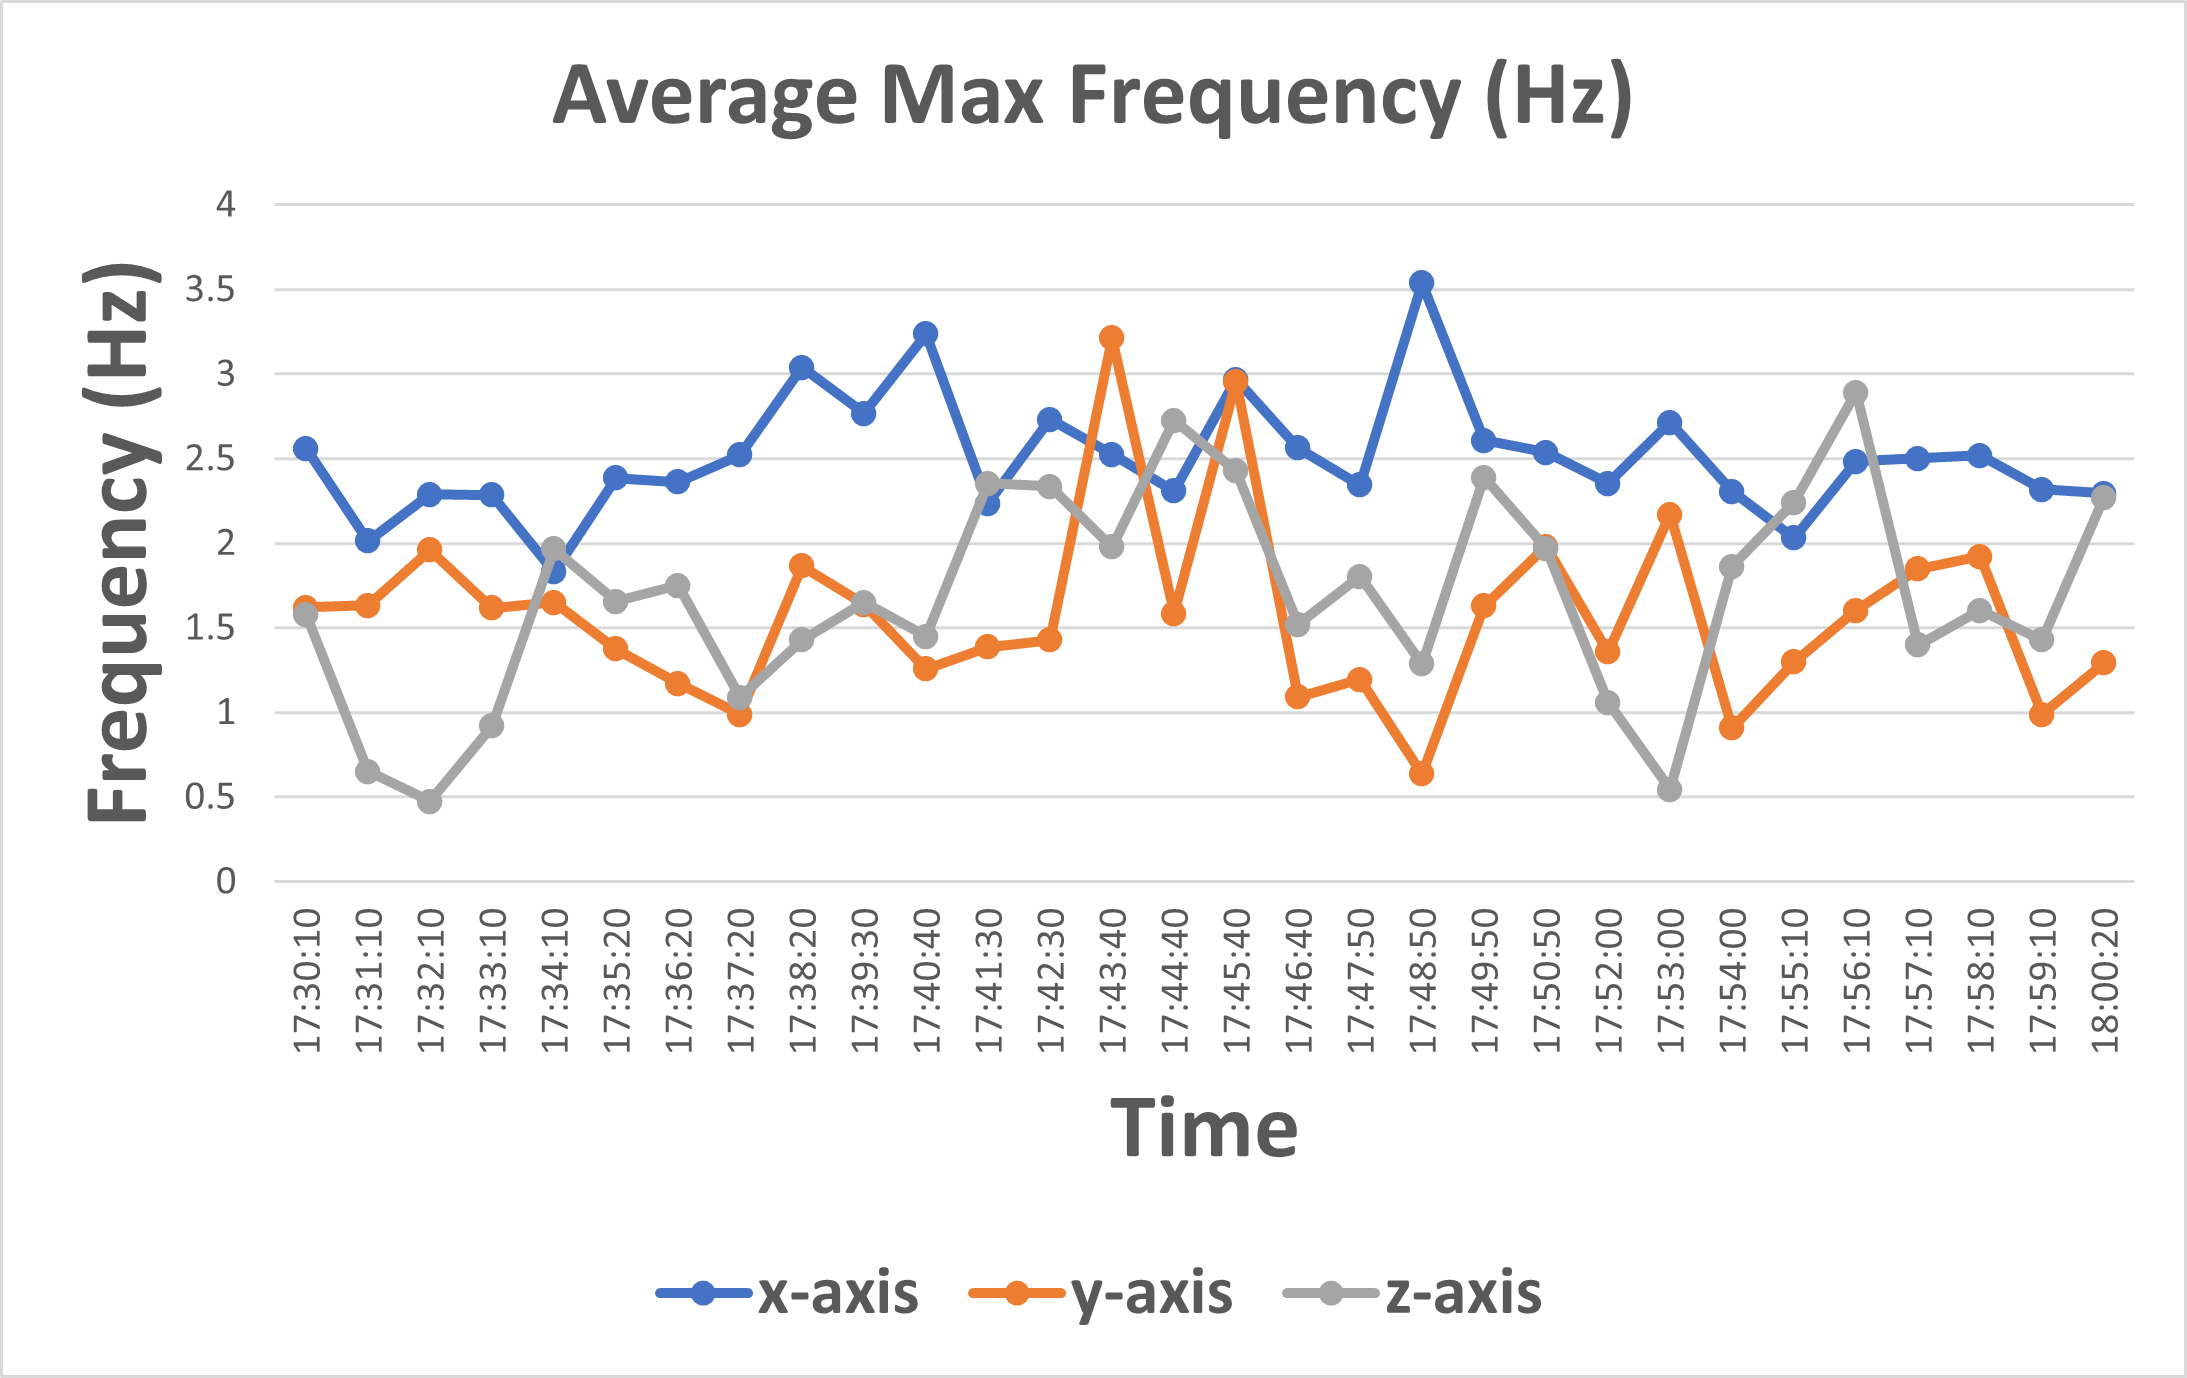
\includegraphics[width=\textwidth]{Sections/Prototype-Testing/proto2-test3-f.png}
	\label{proto2-test3-f}
\end{figure}

\begin{figure}[H]
	\centering
	\caption{Prototype 2: Test 3 SNR}
	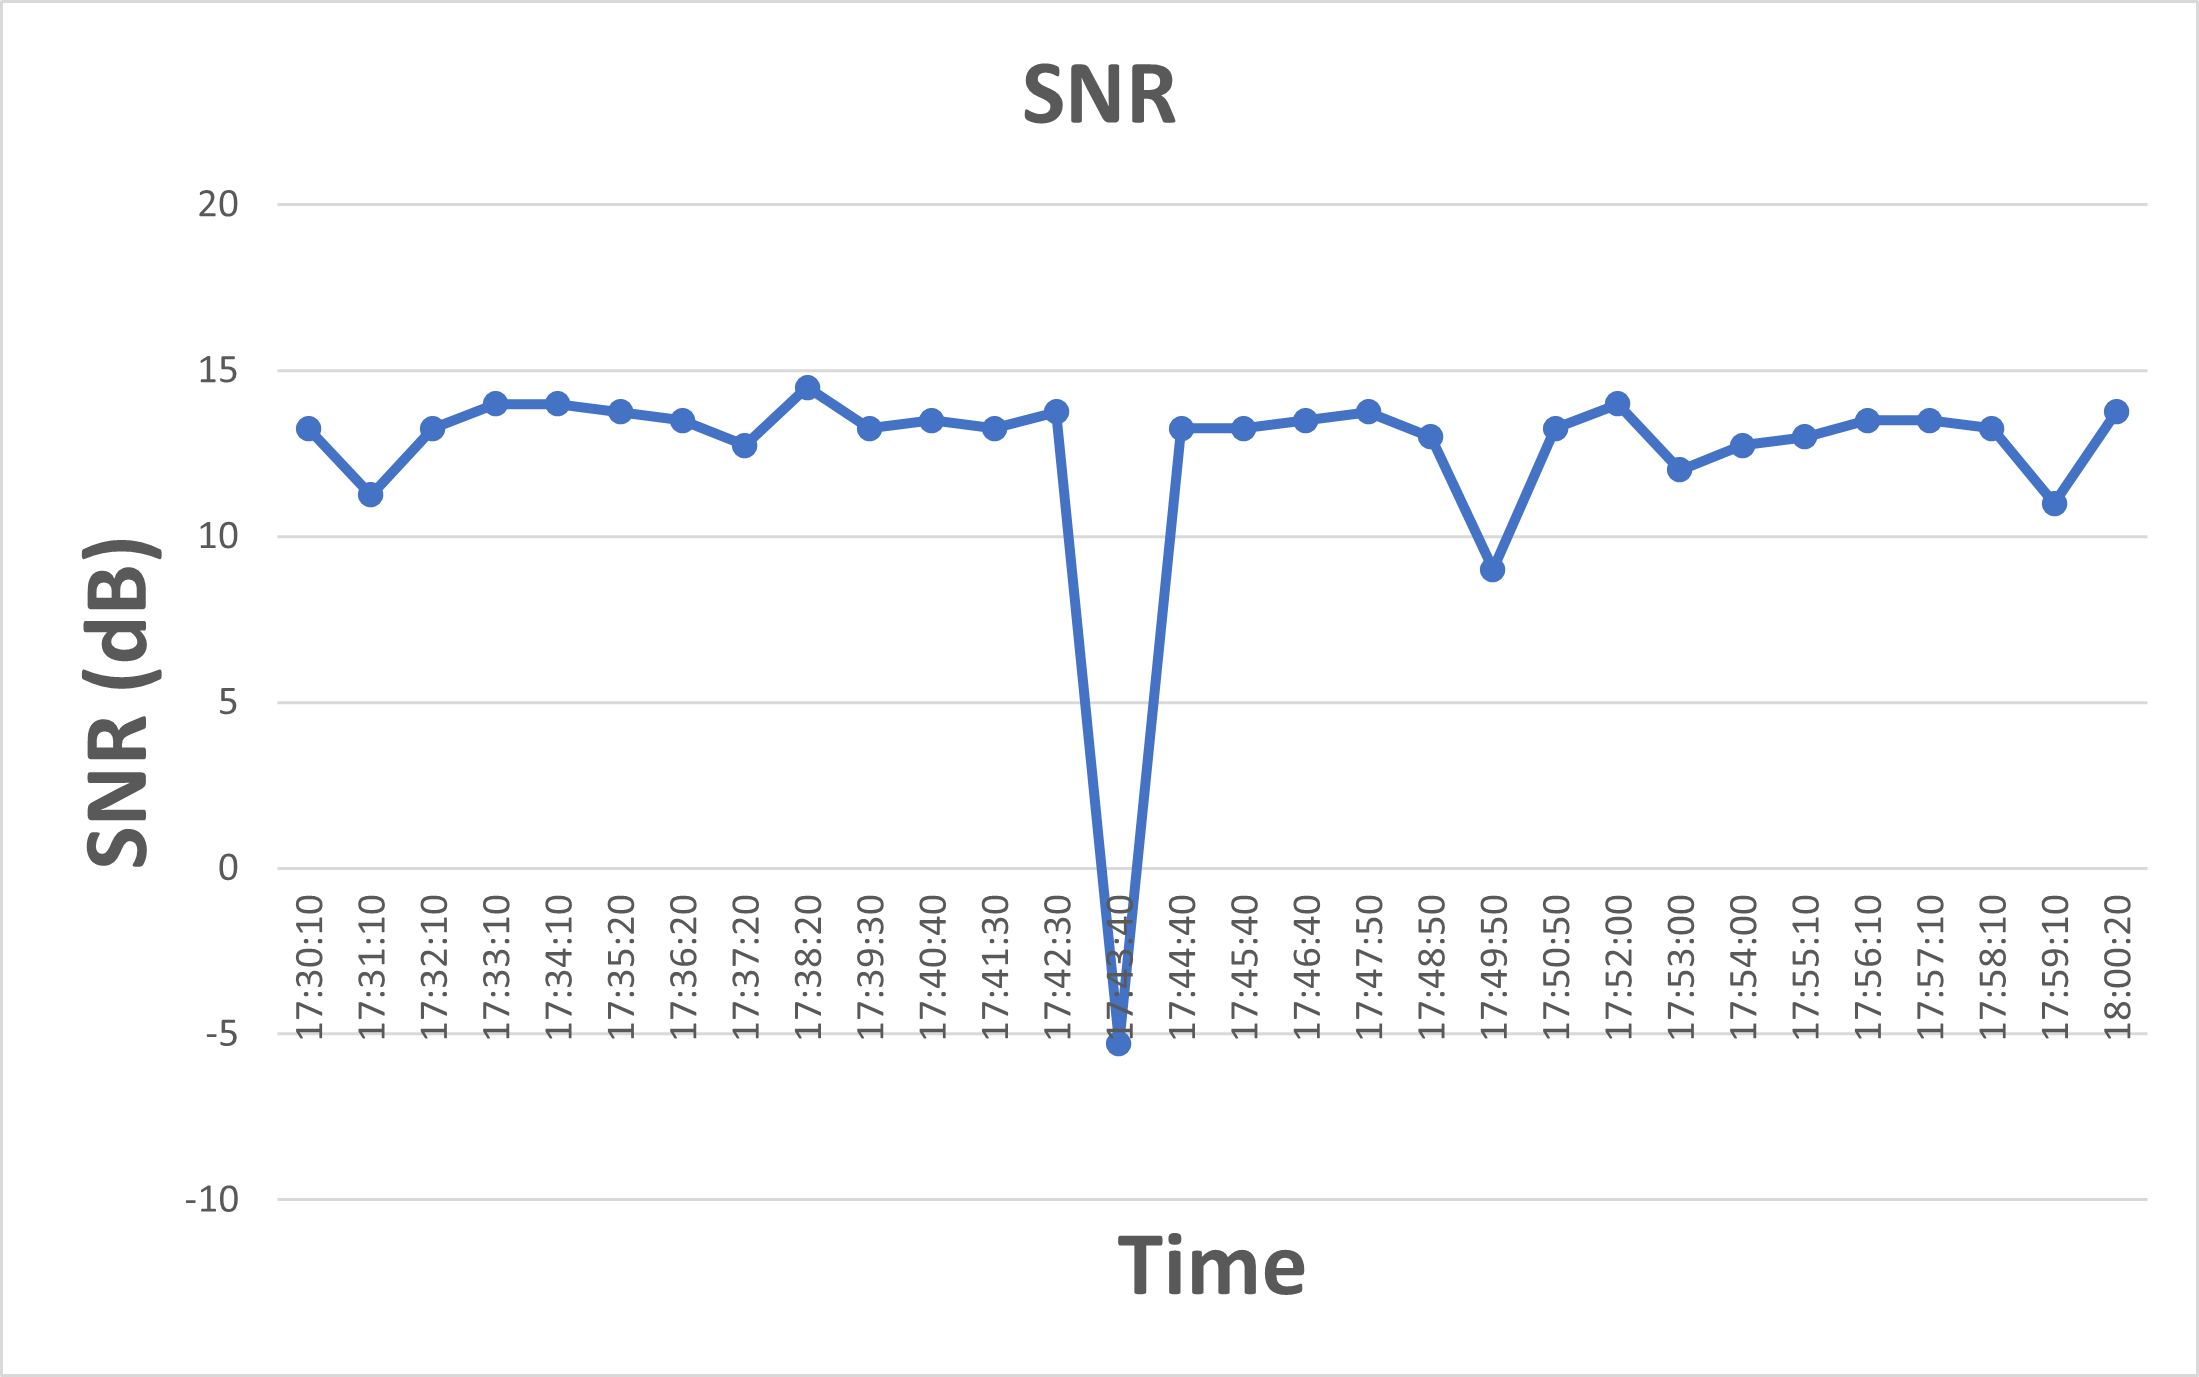
\includegraphics[width=\textwidth]{Sections/Prototype-Testing/proto2-test3-snr.png}
	\label{proto2-test3-snr}
\end{figure}

\begin{figure}[H]
	\centering
	\caption{Prototype 2: Test 3 RSSI}
	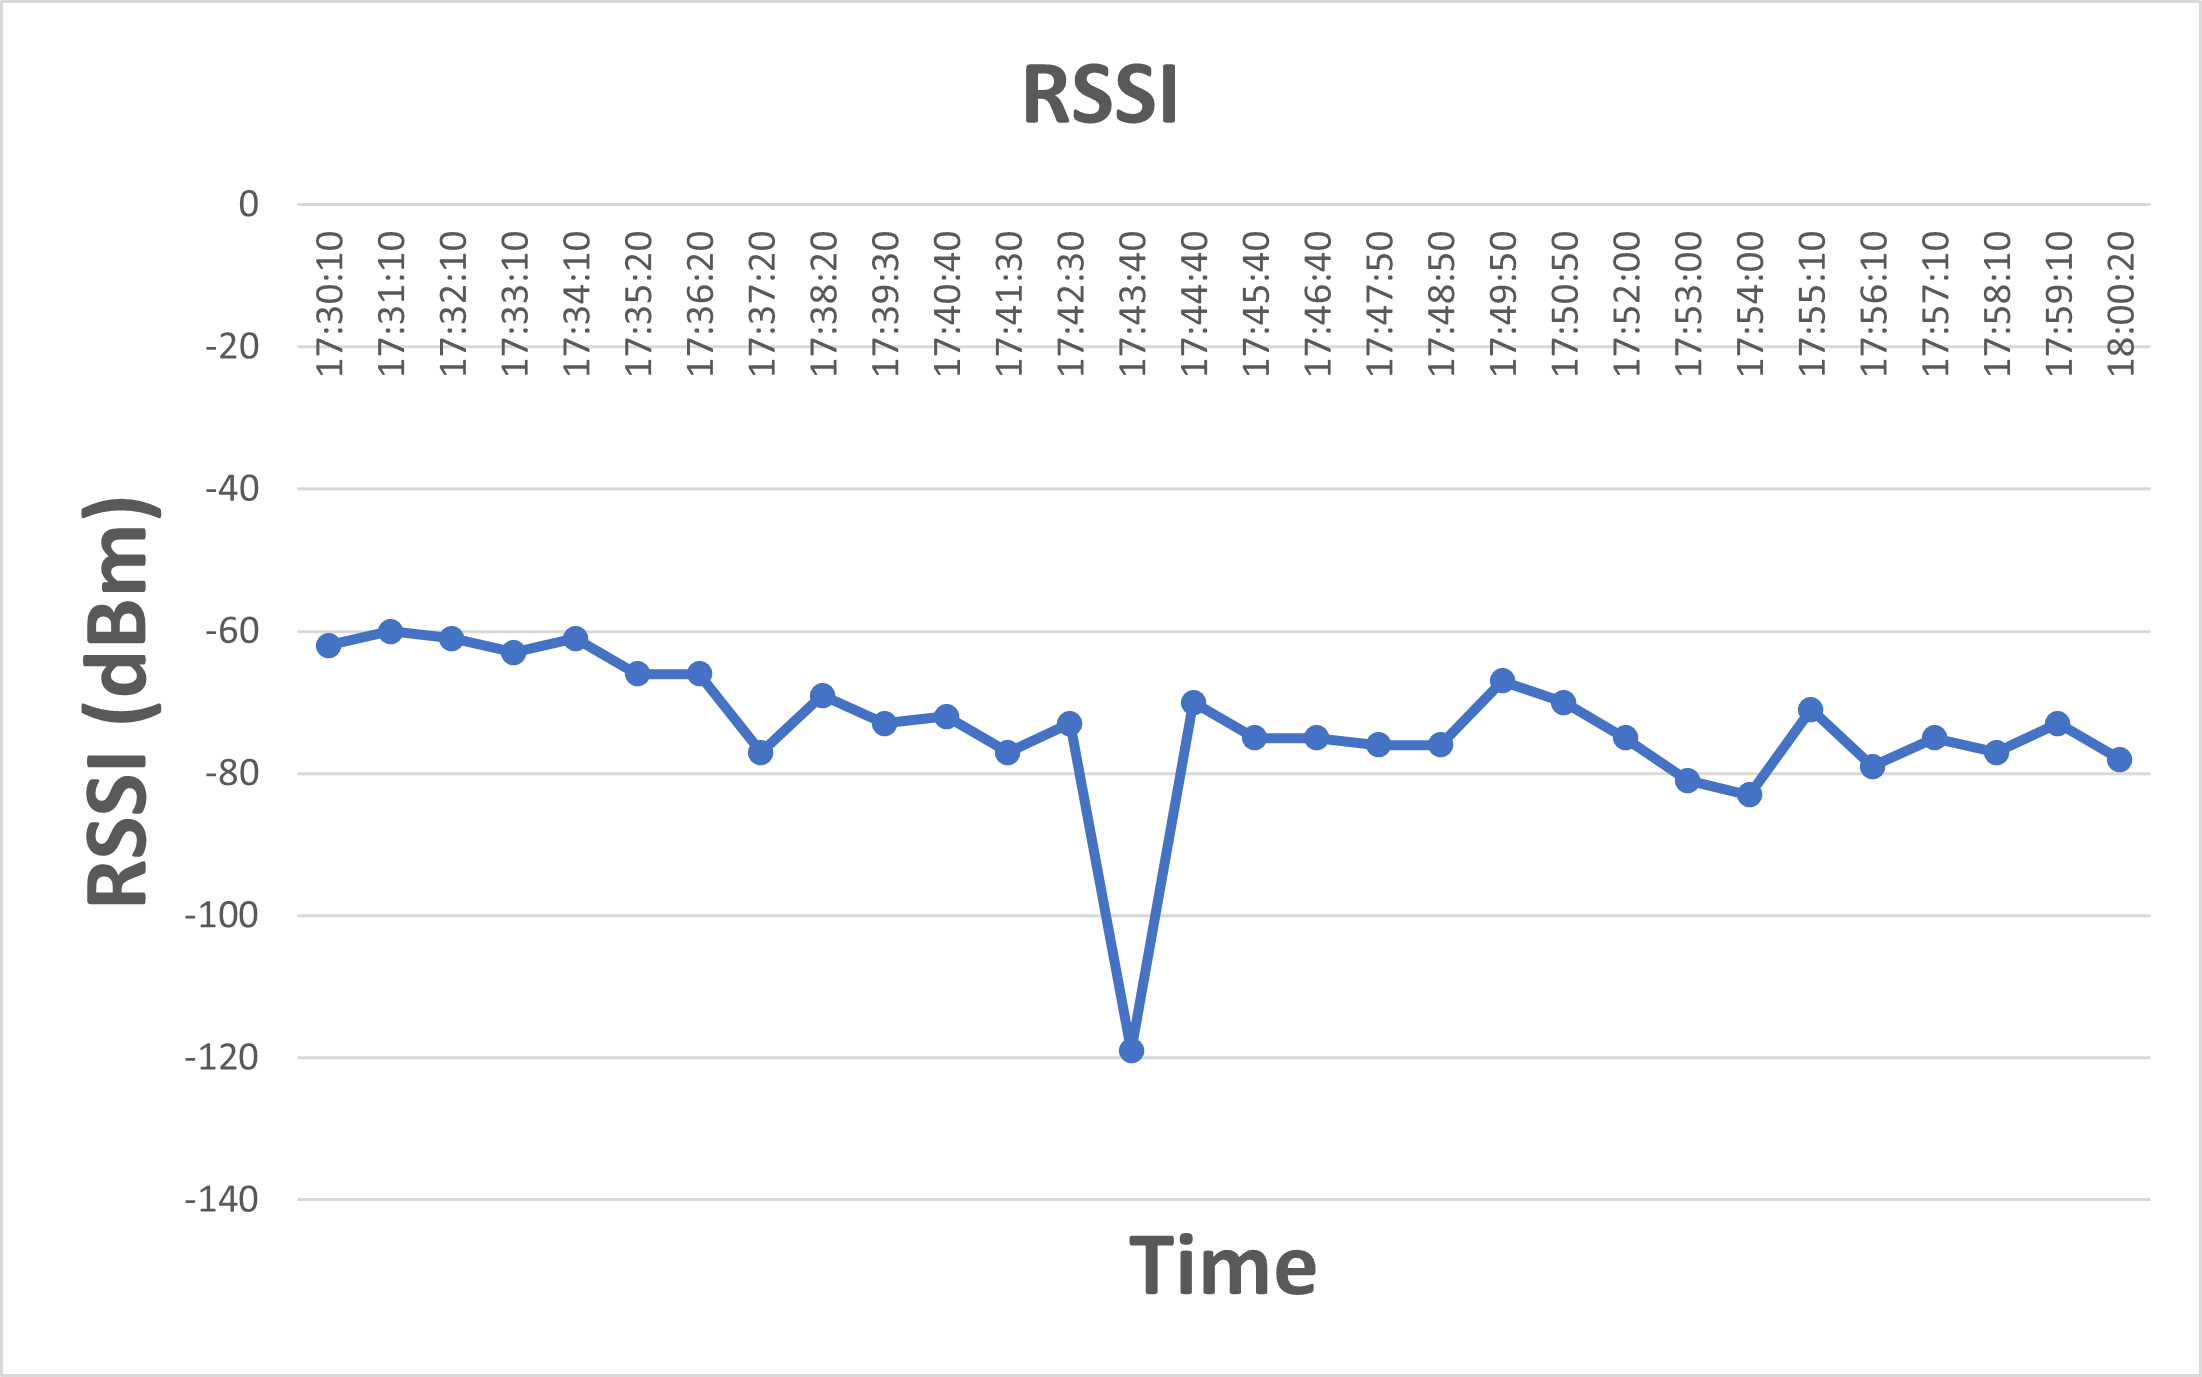
\includegraphics[width=\textwidth]{Sections/Prototype-Testing/proto2-test3-rssi.png}
	\label{proto2-test3-rssi}
\end{figure}










